% \documentclass[handout, xcolor=table]{beamer}
\documentclass[xcolor=table]{beamer}

\usepackage{fixcmex} % fix binomials
\usepackage{xskak}

%-----------------------[ Macros ]----------------------------------------------%

%-----------------------[ Packages ]-------------------------------------------%

% \usepackage[utf8]{inputenc} % not needed for LuaLaTex
\usepackage[brazilian]{babel}
% \usepackage[english]{babel}
\usepackage[T1]{fontenc}
\usepackage{lmodern}
\usepackage{amsfonts}
\usepackage{indentfirst}
\usepackage{xspace}
\usepackage{setspace}
\usepackage{geometry}
\usepackage{mathtools}
\usepackage{amsmath}
\usepackage{amsthm}
\usepackage{subcaption}
\usepackage{pdfpages}
\usepackage{hanging}
\usepackage{pdfpages}
\usepackage{nicefrac}
\usepackage{graphicx}
\usepackage[labelformat=empty]{caption}
\usepackage[shortlabels]{enumitem}
\usepackage{booktabs, multirow} % for borders and merged ranges
% \usepackage[hyperpageref]{backref}
% \usepackage[
%   scr=boondox, % heavily sloped
%   cal=esstix % slightly sloped
% ]{mathalpha}
\usepackage{xmpmulti}
\usepackage{appendixnumberbeamer}
\usepackage{emoji}
% \usepackage{newpxtext} % other font

% Tikz:
\usepackage{tikz}
% \usetikzlibrary{ipe} % ipe compatibility library
\usetikzlibrary{calc, arrows, arrows.meta, patterns}

\usepackage{macrossty}

%-----------------------[ Colors ]---------------------------------------------%

\definecolor{red}{rgb}{1,0,0}
\definecolor{blue}{rgb}{0,0,1}
\definecolor{green}{rgb}{0,1,0}
\definecolor{yellow}{rgb}{1,1,0}
\definecolor{orange}{rgb}{1,0.647,0}
\definecolor{gold}{rgb}{1,0.843,0}
\definecolor{purple}{rgb}{0.627,0.125,0.941}
\definecolor{gray}{rgb}{0.745,0.745,0.745}
\definecolor{brown}{rgb}{0.647,0.165,0.165}
\definecolor{navy}{rgb}{0,0,0.502}
\definecolor{pink}{rgb}{1,0.753,0.796}
\definecolor{seagreen}{rgb}{0.18,0.545,0.341}
\definecolor{turquoise}{rgb}{0.251,0.878,0.816}
\definecolor{violet}{rgb}{0.933,0.51,0.933}
\definecolor{darkblue}{rgb}{0,0,0.545}
\definecolor{darkcyan}{rgb}{0,0.545,0.545}
\definecolor{darkgray}{rgb}{0.663,0.663,0.663}
\definecolor{darkgreen}{rgb}{0,0.392,0}
\definecolor{darkmagenta}{rgb}{0.545,0,0.545}
\definecolor{darkorange}{rgb}{1,0.549,0}
\definecolor{darkred}{rgb}{0.545,0,0}
\definecolor{lightblue}{rgb}{0.678,0.847,0.902}
\definecolor{lightcyan}{rgb}{0.878,1,1}
\definecolor{lightgray}{rgb}{0.827,0.827,0.827}
\definecolor{lightgreen}{rgb}{0.565,0.933,0.565}
\definecolor{lightyellow}{rgb}{1,1,0.878}
\definecolor{black}{rgb}{0,0,0}
\definecolor{white}{rgb}{1,1,1}

%-----------------------[ Commands ]-------------------------------------------%

\newcommand\mycomment[1]{} % block comment

\newcommand{\dist}{\text{dist}}
\newcommand{\cost}{\text{cost}}
\newcommand{\opt}{\text{OPT}}
\newcommand{\makespan}{\emph{makespan}}

\newcommand{\cala}{\mathcal{A}}
\newcommand{\calb}{\mathcal{B}}
\newcommand{\calg}{\mathcal{G}}
\newcommand{\cali}{\mathcal{I}}
\newcommand{\call}{\mathcal{L}}
\newcommand{\calo}{\mathcal{O}}
\newcommand{\cals}{\mathcal{S}}
\newcommand{\calt}{\mathcal{T}}

\newcommand{\N}{\rm I\!N}
\newcommand{\overeps}{\nicefrac{1}{\varepsilon}}
\newcommand{\B}{$\bullet$}

\newcommand\rest[2]{\left.{#1}\right|_{#2}} % function restriction

\newcommand\set[1]{\{#1\}}

\DeclarePairedDelimiter\ceil{\lceil}{\rceil}
\DeclarePairedDelimiter\floor{\lfloor}{\rfloor}
\DeclareMathOperator*{\argmax}{arg\,max}
\DeclareMathOperator*{\argmin}{arg\,min}

\newcommand{\XSAT}{\textrm{XSAT}} % Exact SAT
\newcommand{\rXSAT}{$(2,1)$-\XSAT} % Exact SAT with 2 positive, 1 negative occurences of each variable
\newcommand{\rXthreeSAT}{\mbox{$1$-in-$3$-SAT$_{(2,1)}$}}%{$(2,1)$-X3SAT} % Exact SAT with 2 positive, 1 negative occurences of each variable, and clauses with size <= 3
\newcommand{\kXSAT}{$k$-\textrm{True} \rXSAT}
\newcommand{\kXthreeSAT}{$k$-\textrm{True} \rXthreeSAT}

%-----------------------[ Proof Environments ]---------------------------------%

\newtheorem{defi}{Definição}
\newtheorem{thm}{Teorema}
\newtheorem{cor}{Corolário}
\newtheorem{conj}{Conjectura}
\newtheorem{lema}{Lema}
\newtheorem{obs}{Observação}
\newtheorem{remark}{Remark}
\newtheorem{proposition}{Proposition}

\newcounter{finalframe}
\newcommand{\stopcounter}{
  \setcounter{finalframe}{\insertframenumber}
}

\newcommand{\resumecounter}{
  \setcounter{framenumber}{\value{finalframe}}
}

\newcommand{\inccounter}{
  \setcounter{framenumber}{\value{finalframe} + 1}
}

%-----------------------[ Template ]-------------------------------------------%

\mode<presentation> {
    \usetheme[sectionpage=none, progressbar=frametitle, block=fill]{moloch} % modern fork of the metropolis theme
    \setbeamertemplate{footline}[frame number] % to replace the footer line in all slides with a simple slide count
}
\setbeamerfont{footnote}{size=\tiny}
\setbeamertemplate{navigation symbols}{}
\setbeamertemplate{footnote}{%
    \hangpara{2em}{1}%
    \makebox[2em][l]{\tiny\insertfootnotemark}%
    \hspace{-1em}\tiny\insertfootnotetext\par\vspace{0.2cm}%
}
\setbeamercolor{background canvas}{bg=white}

% Enumerate setup:
\def\labelenumi{\textbf{\arabic{enumi}.}}

% Lists setup:
\beamerdefaultoverlayspecification{<+->}

%-----------------------[ (Sub)Section Slides ]--------------------------------%

\AtBeginSection[]{
    \begin{frame}
    \vfill
    \centering
    \setbeamercolor{title}{bg=mDarkTeal,fg=black!2}
    \begin{beamercolorbox}[sep=8pt,center,shadow=true]{title}
        \usebeamerfont{title}\insertsectionhead\par%
    \end{beamercolorbox}
    \vfill
    \end{frame}
}

% \makeatletter
% \newcommand{\subseqslide}{
% \begin{frame}
%   \setbeamercolor{title}{bg=mDarkTeal,fg=black!2}
%   \centering
%   \begin{minipage}{22em}
%     \raggedright
%     \begin{beamercolorbox}[sep=8pt,center,shadow=true]{title}
%         \usebeamerfont{title}\insertsectionhead\par%
%     \end{beamercolorbox}
%     \usebeamertemplate*{progress bar in section page}
%     \par
%     \ifx\insertsubsectionhead\@empty\else%
%       \vskip-.6\baselineskip
%       \usebeamercolor[fg]{subsection title}%
%       \usebeamerfont{subsection title}%
%       \insertsubsectionhead{}
%     \fi
%   \end{minipage}
%   \par
%   \vspace{\baselineskip}
% \end{frame}
% }

% \AtBeginSubsection[]{%
% \subseqslide

% \setcounter{tocdepth}{3}
% \frame<beamer>{ 
%   \frametitle{}
%   \centering
%   \begin{minipage}{20em}
%   \tableofcontents[
%     currentsection,currentsubsection,sectionstyle=show/hide,subsectionstyle=show/shaded/hide,subsubsectionstyle=show/show/hide/hide
%   ]    
%   \end{minipage}
% }
% }
% \makeatother

%-----------------------[ Title page ]-----------------------------------------%

\title{Técnica de \emph{Shifting}}

\titlegraphic{
  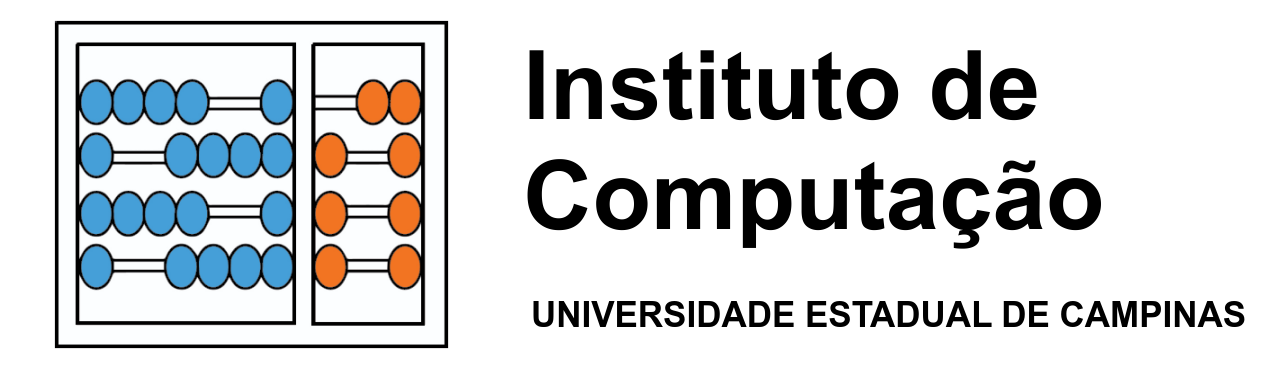
\includegraphics[height=1.cm]{logos/ic.png}
  \hfill
  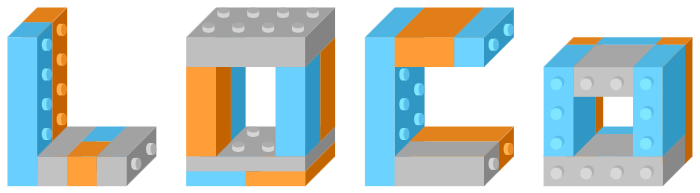
\includegraphics[height=0.85cm]{logos/loco.png}
}

\author{
Lucas de Oliveira Silva - 220715
\and \\
Ricardo Andres Marino Rojas - 175824
}

\institute{MO829 - Algoritmos Parametrizados}

\date{\vfill\hfill 1° de Julho de 2025}

\begin{document}

\hyphenpenalty=10000

\begin{frame}[plain]
  \titlepage
\end{frame}

%------------------------------------------------------------------------------%

\section{Introdução}
\begin{frame}{Problema Exemplo}
    \defproblemaOPT
        {Conjunto Independente Máximo (CI)}
        {Grafo $G = (V, E)$.\pause}
        {$S \subseteq V$ tal que $|E(G[S])|=0$, com $|S|$ máximo.}
\end{frame}

\begin{frame}{Dificuldade}
    \begin{thm}[\cite{Ga79}]
        O problema CI é NP-difícil, mesmo em grafos cúbicos e planares.
    \end{thm}
\end{frame}

\begin{frame}{Dificuldade Parametrizada}
    \begin{thm}[\cite{Cygan15}]
        O problema CI parametrizado pelo tamanho da solução $k$ é $W[1]$-completo.
    \end{thm}
\end{frame}

\begin{frame}{Outras Classes de Grafos}
    -- CI em árvores?\\
    \pause
    \hfill EZ --\\
    \pause \bigbreak
    \Large
    -- E quanto a outras classes?\\
    \pause
    \hfill Você já ouviu falar de grafos planares? --
\end{frame}


\section{Preliminares}
\begin{frame}{Grafos Planares}
    \centering\Large
    Um grafo é \textbf{\emph{planar}} se ele pode ser desenhado no plano Euclidiano sem cruzamentos de arestas.
    \bigbreak
    
    \begin{columns}
        \column{0.5\textwidth}
        \begin{figure}
            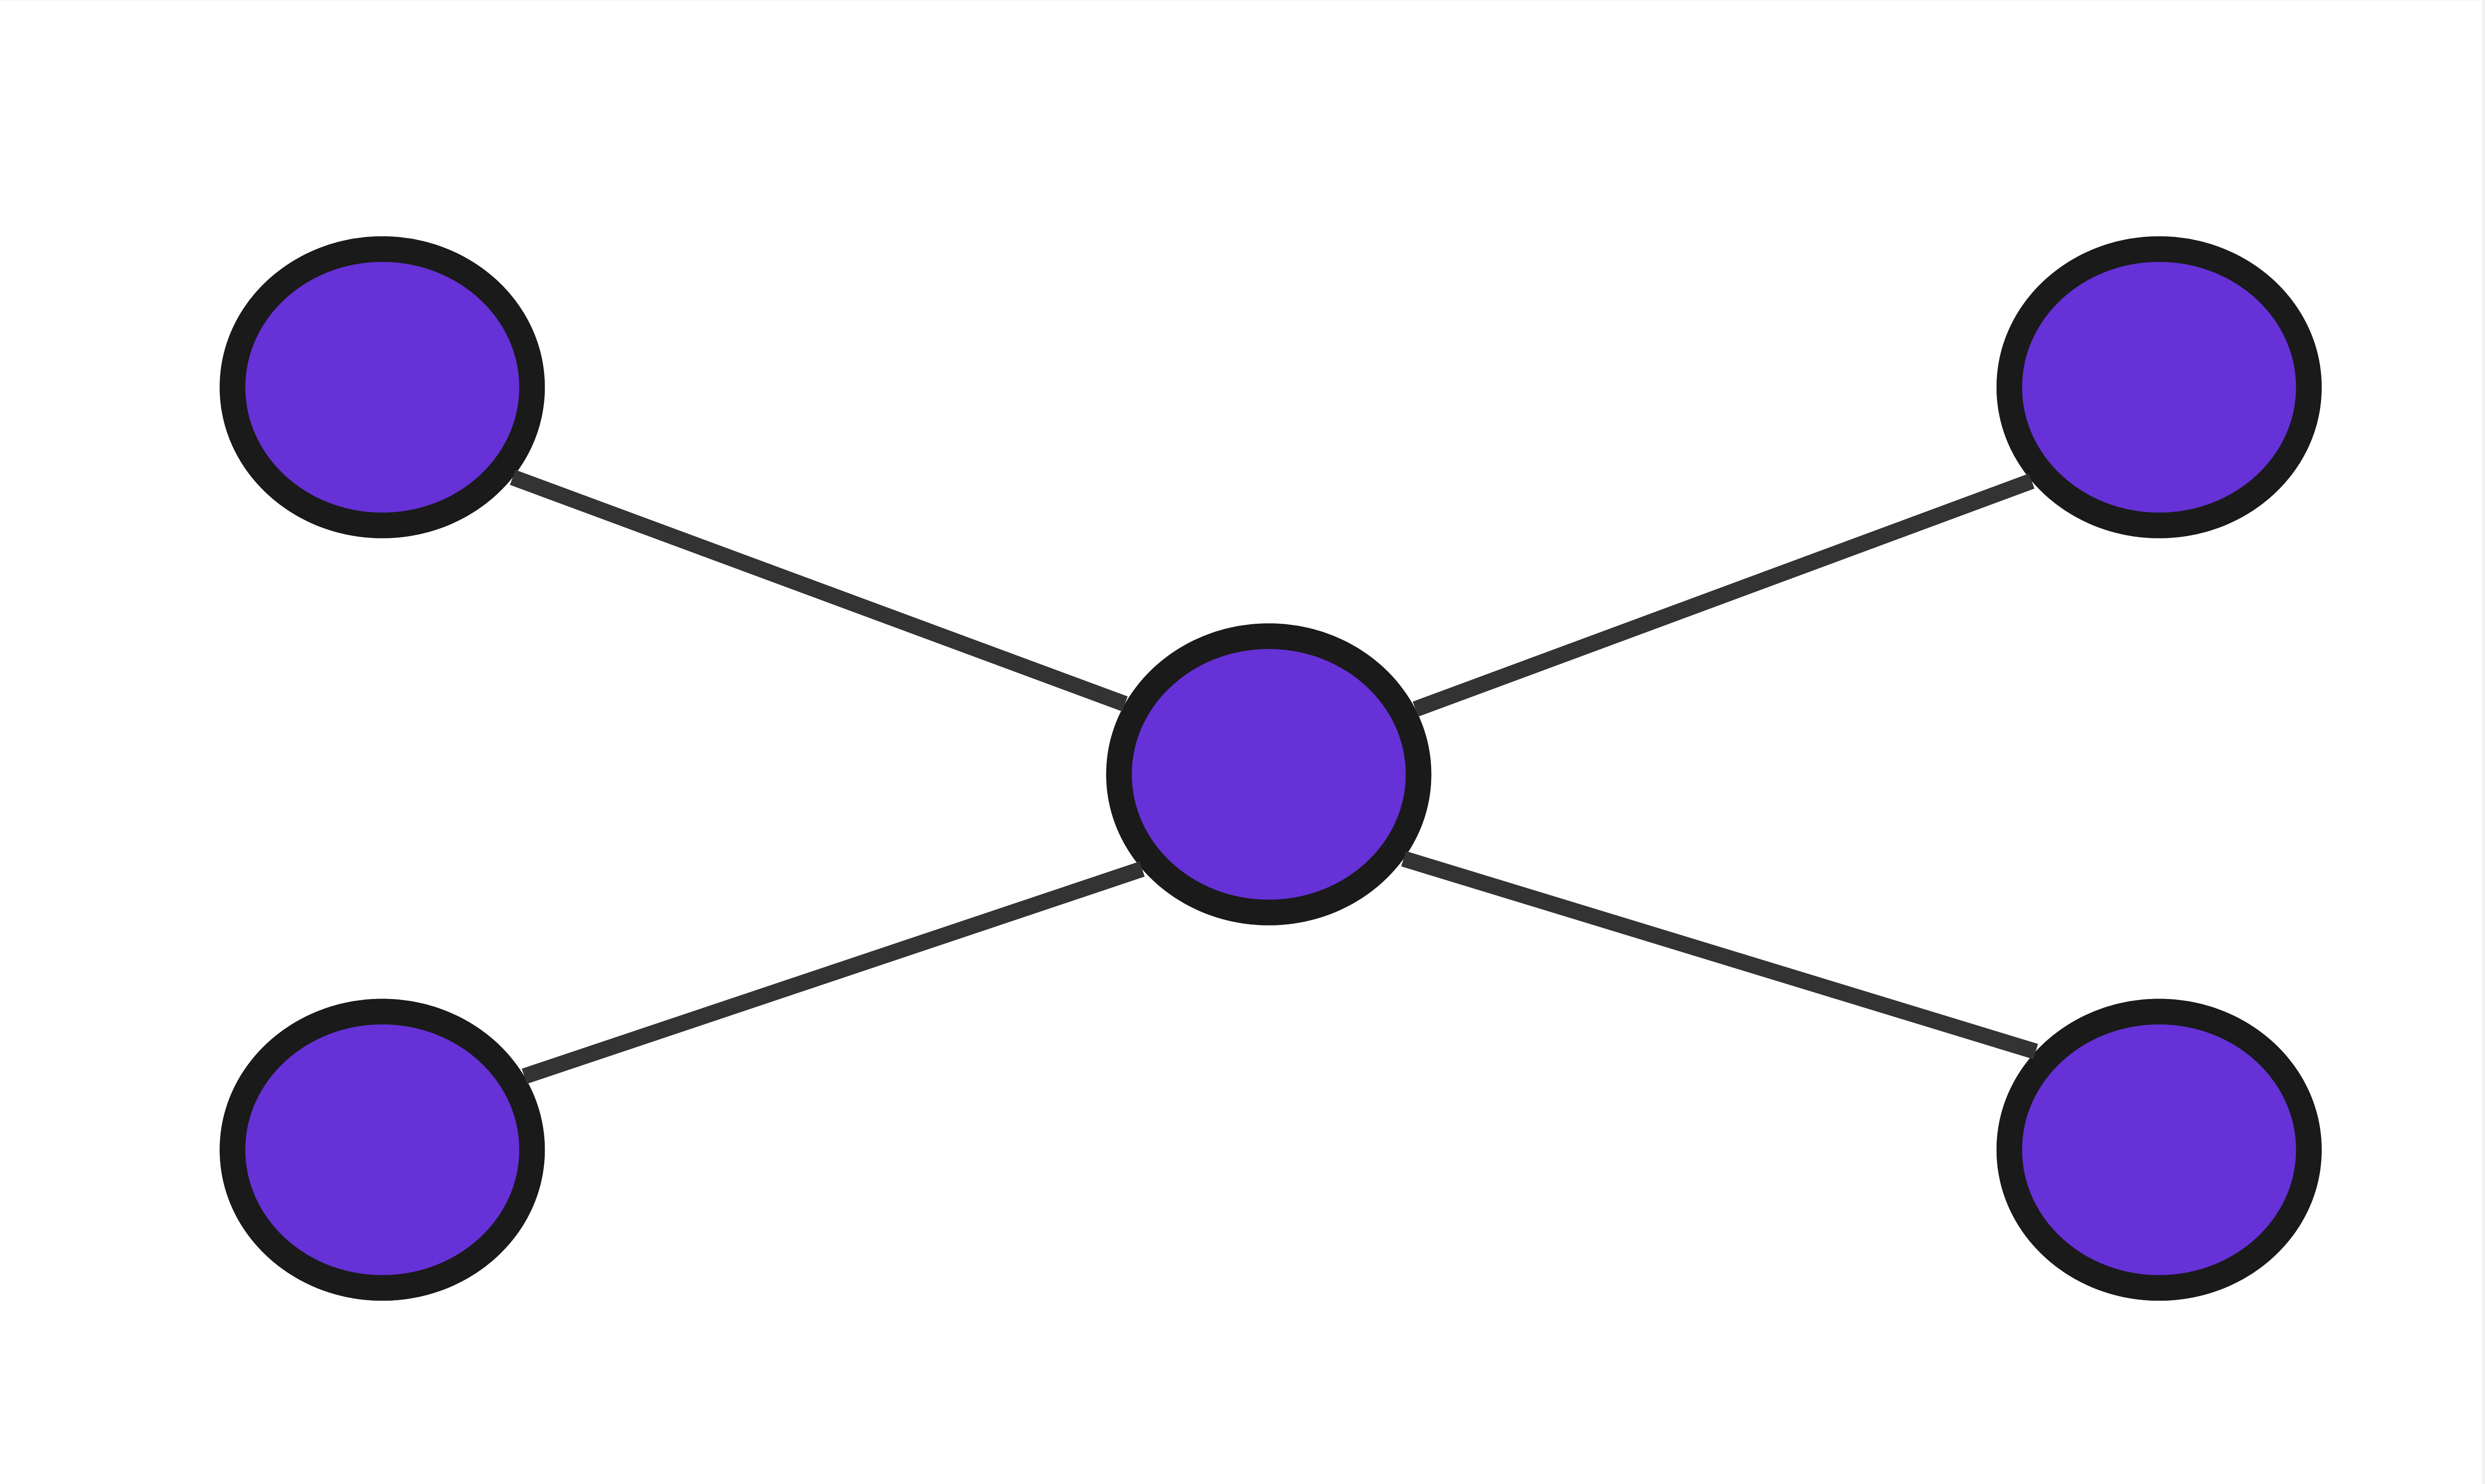
\includegraphics[width=0.9\linewidth]{images/butterfly_graph.jpg}
            \caption*{\textit{Grafo Borboleta}}
        \end{figure}
    
        \column{0.5\textwidth}
        \begin{figure}
            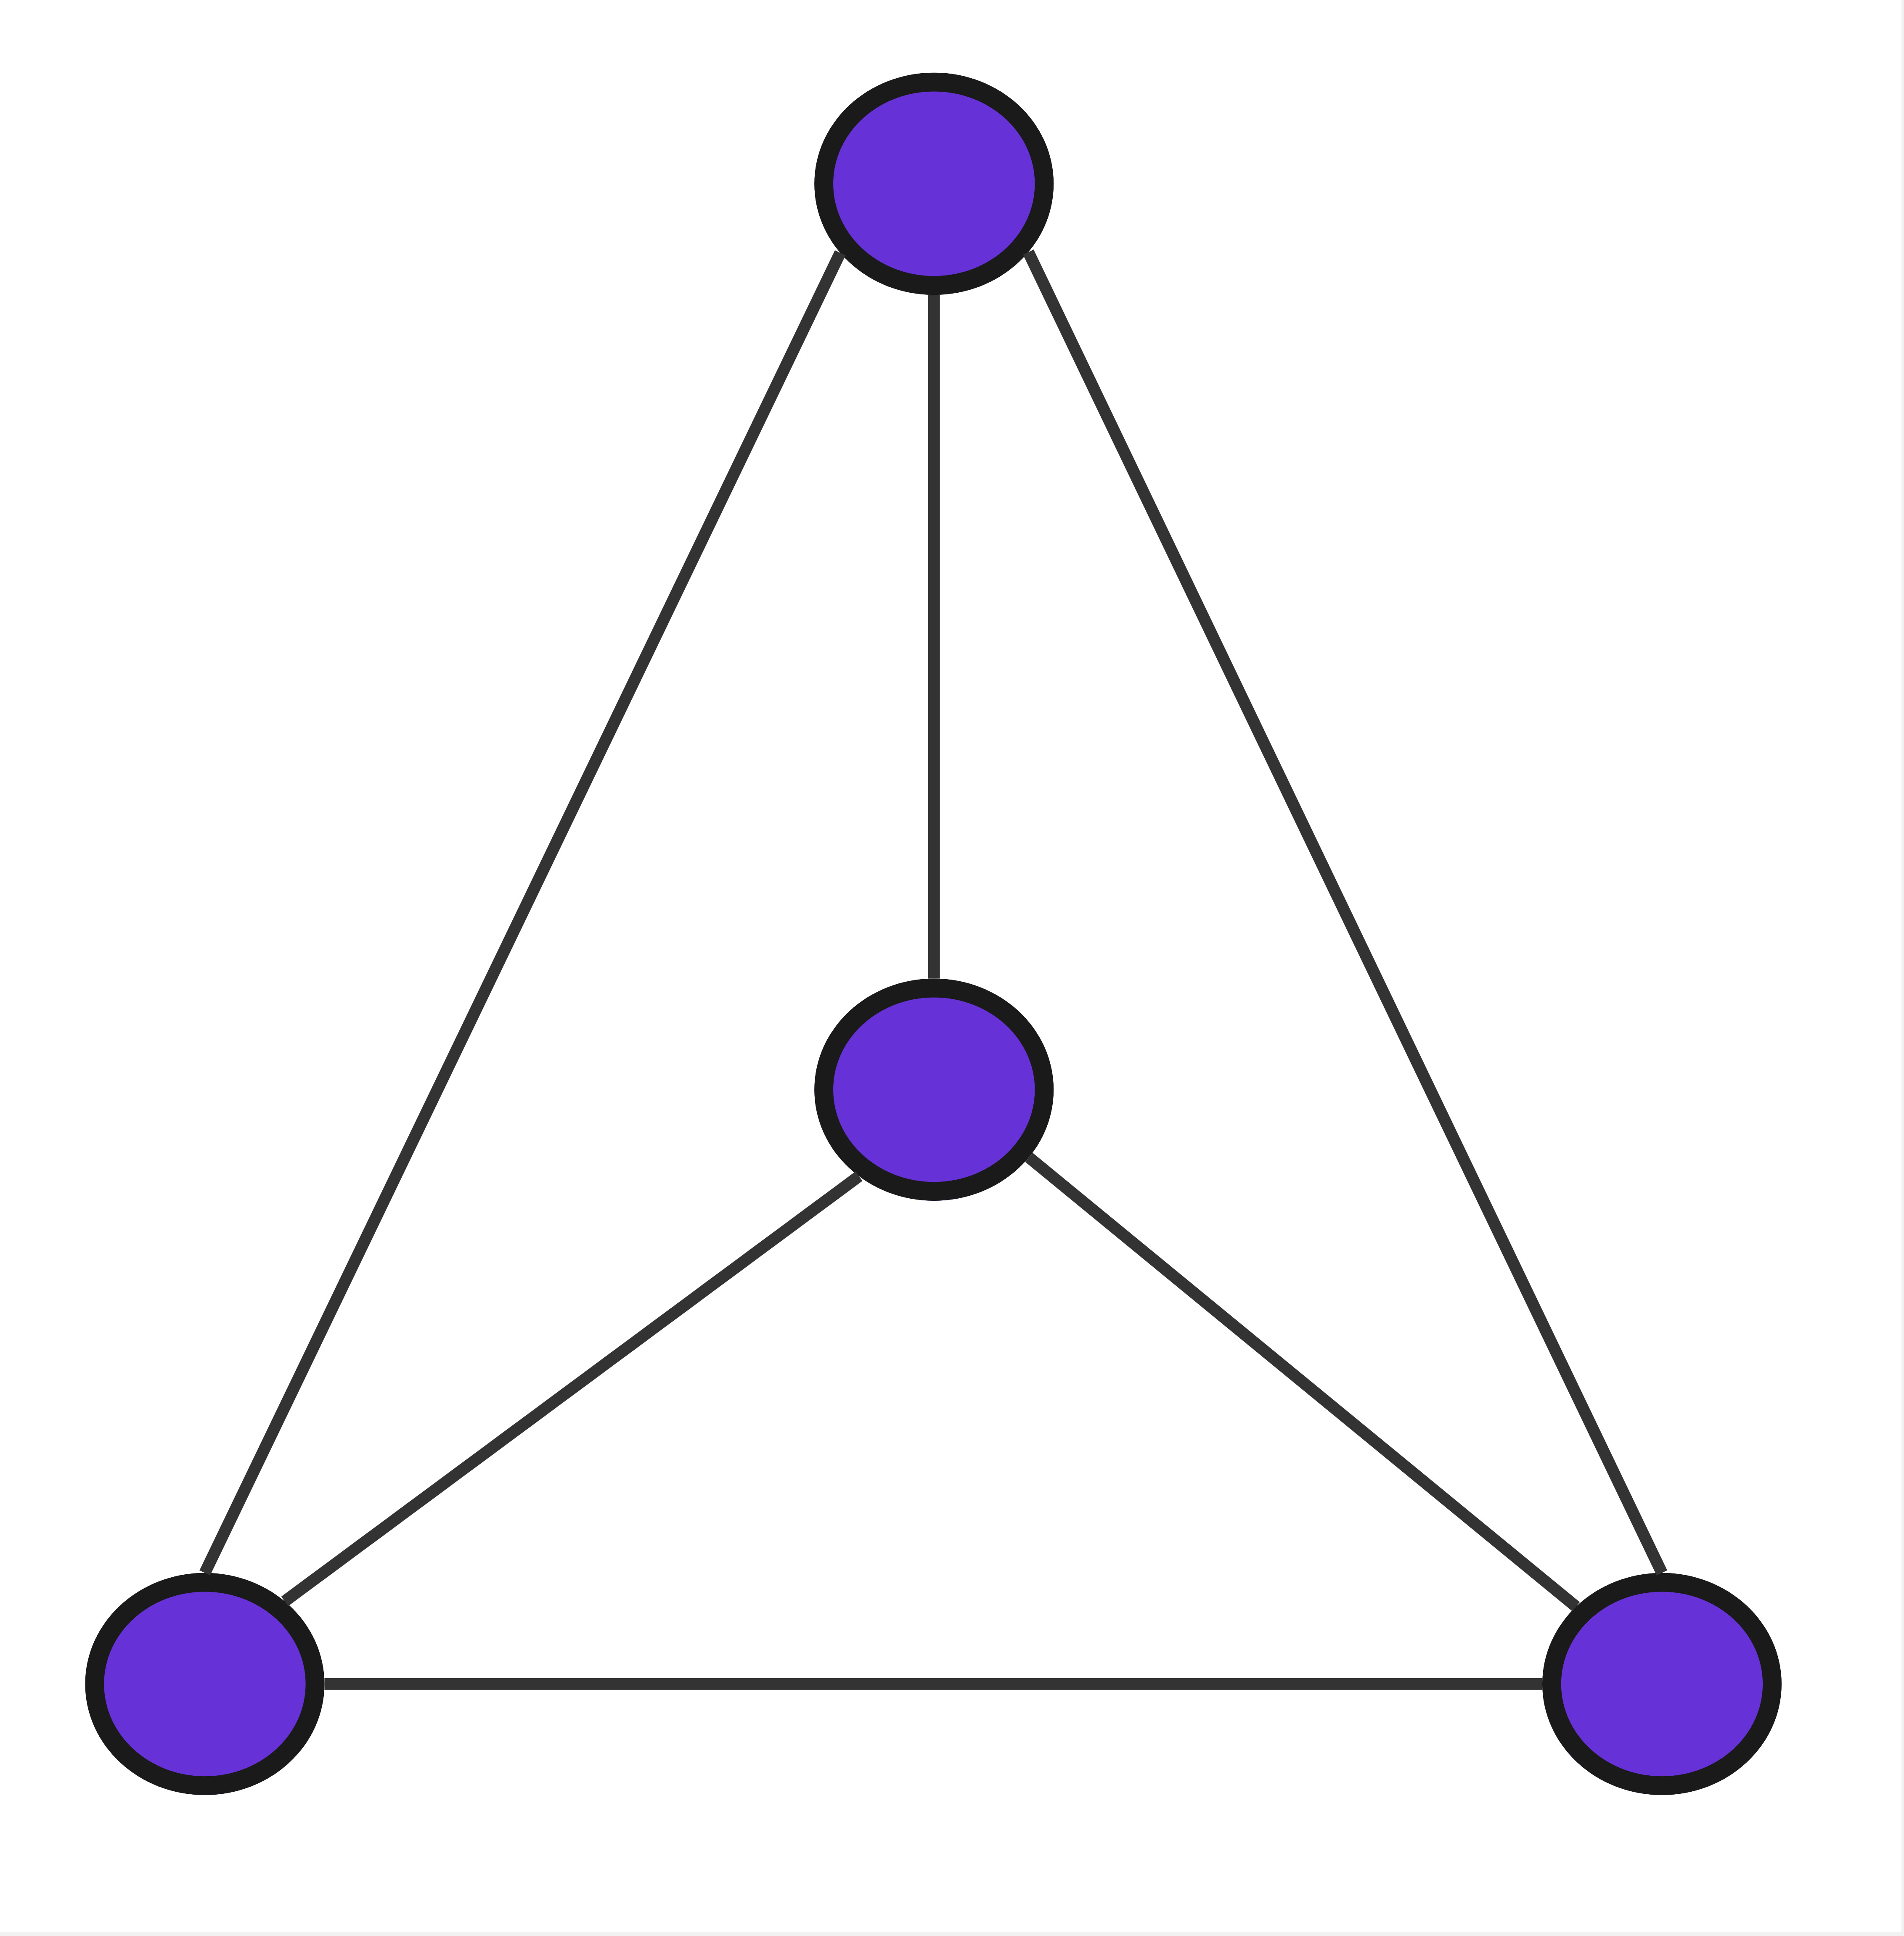
\includegraphics[width=0.9\linewidth]{images/k4_graph.jpg}
            \caption*{\textit{$K_4$}}
        \end{figure}
    \end{columns}
\end{frame}

\begin{frame}{Quiz}
  \centering
  \Large
  Qual dos três grafos a seguir é planar?
  \bigbreak
  \begin{minipage}{\linewidth}
    \centering
    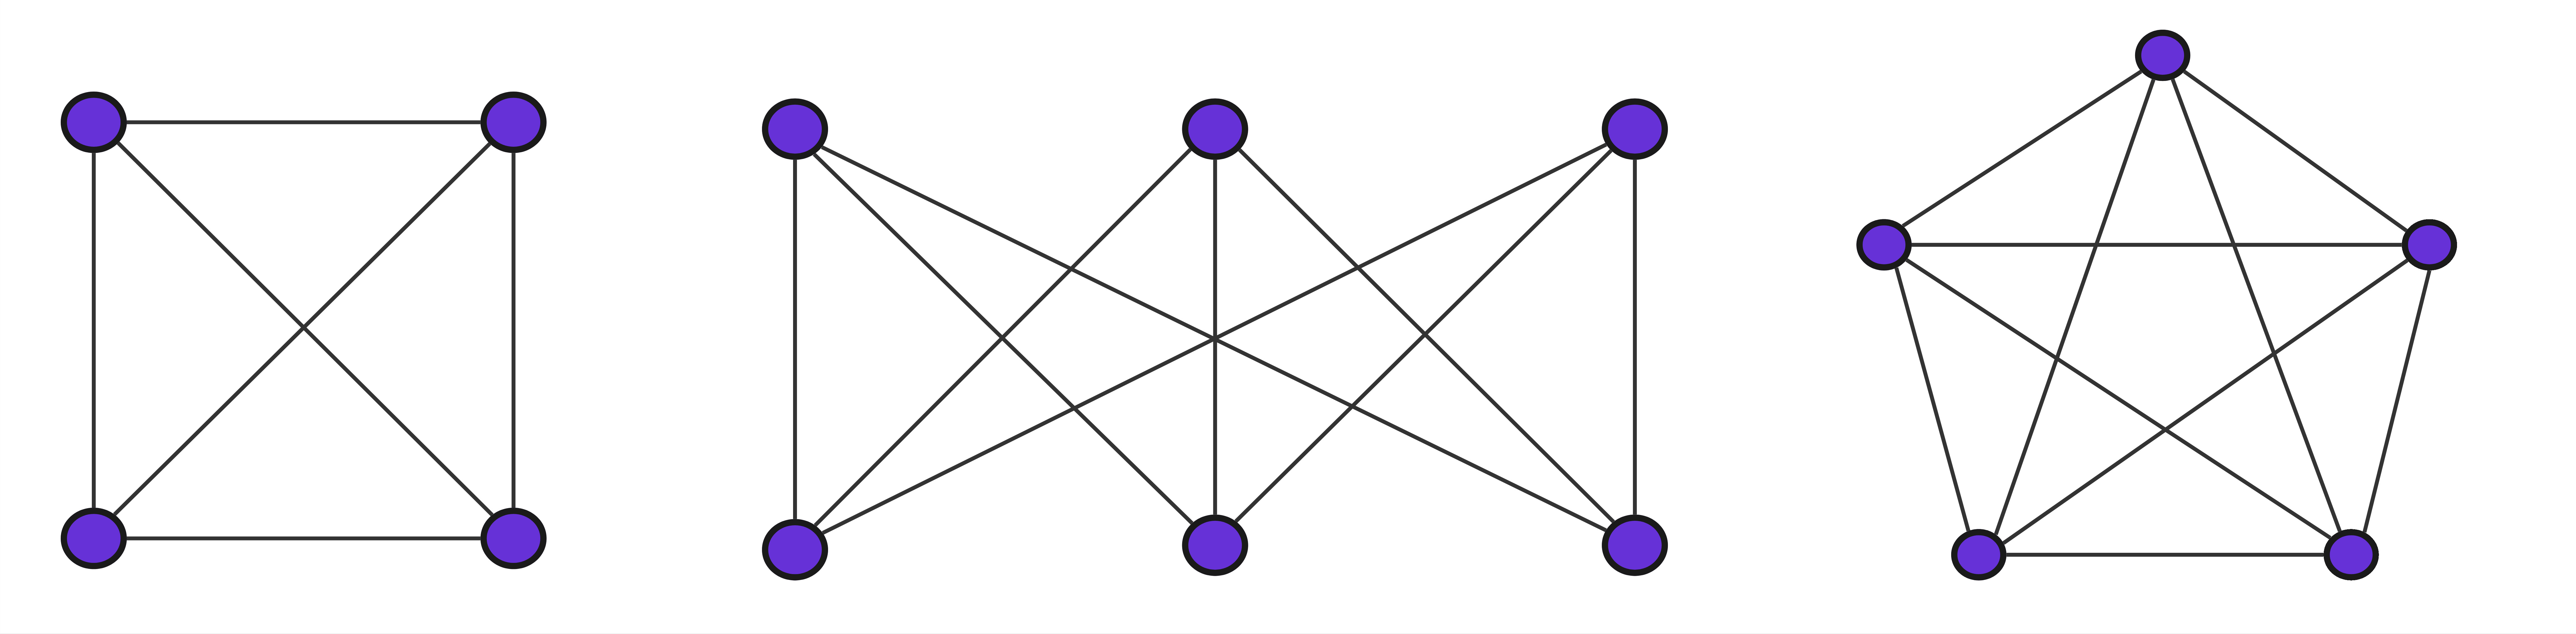
\includegraphics[height=2.5cm]{images/quiz_1.jpg}
  \end{minipage}
\end{frame}

\begin{frame}{Quiz}
  \centering
  \Large
  Qual dos três grafos a seguir é planar?
  \bigbreak
  \begin{minipage}{\linewidth}
    \centering
    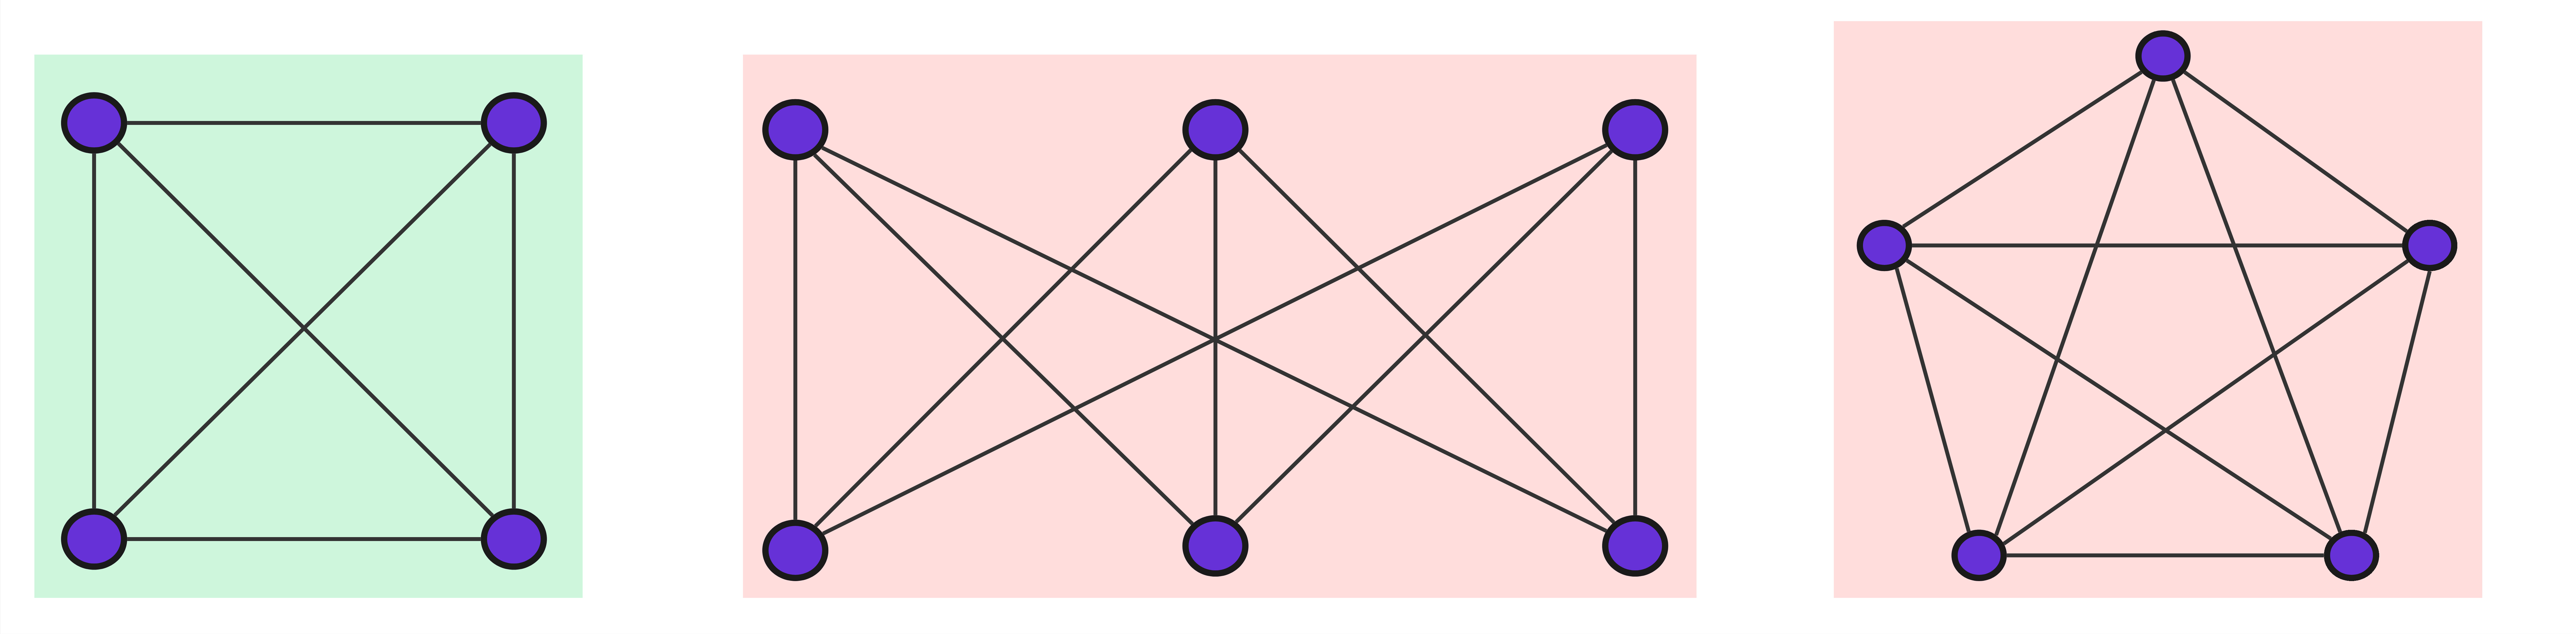
\includegraphics[height=2.5cm]{images/quiz_1_solved.jpg}
  \end{minipage}
\end{frame}

\begin{frame}{Mais Definições}
    \begin{minipage}{\linewidth}
        \centering
        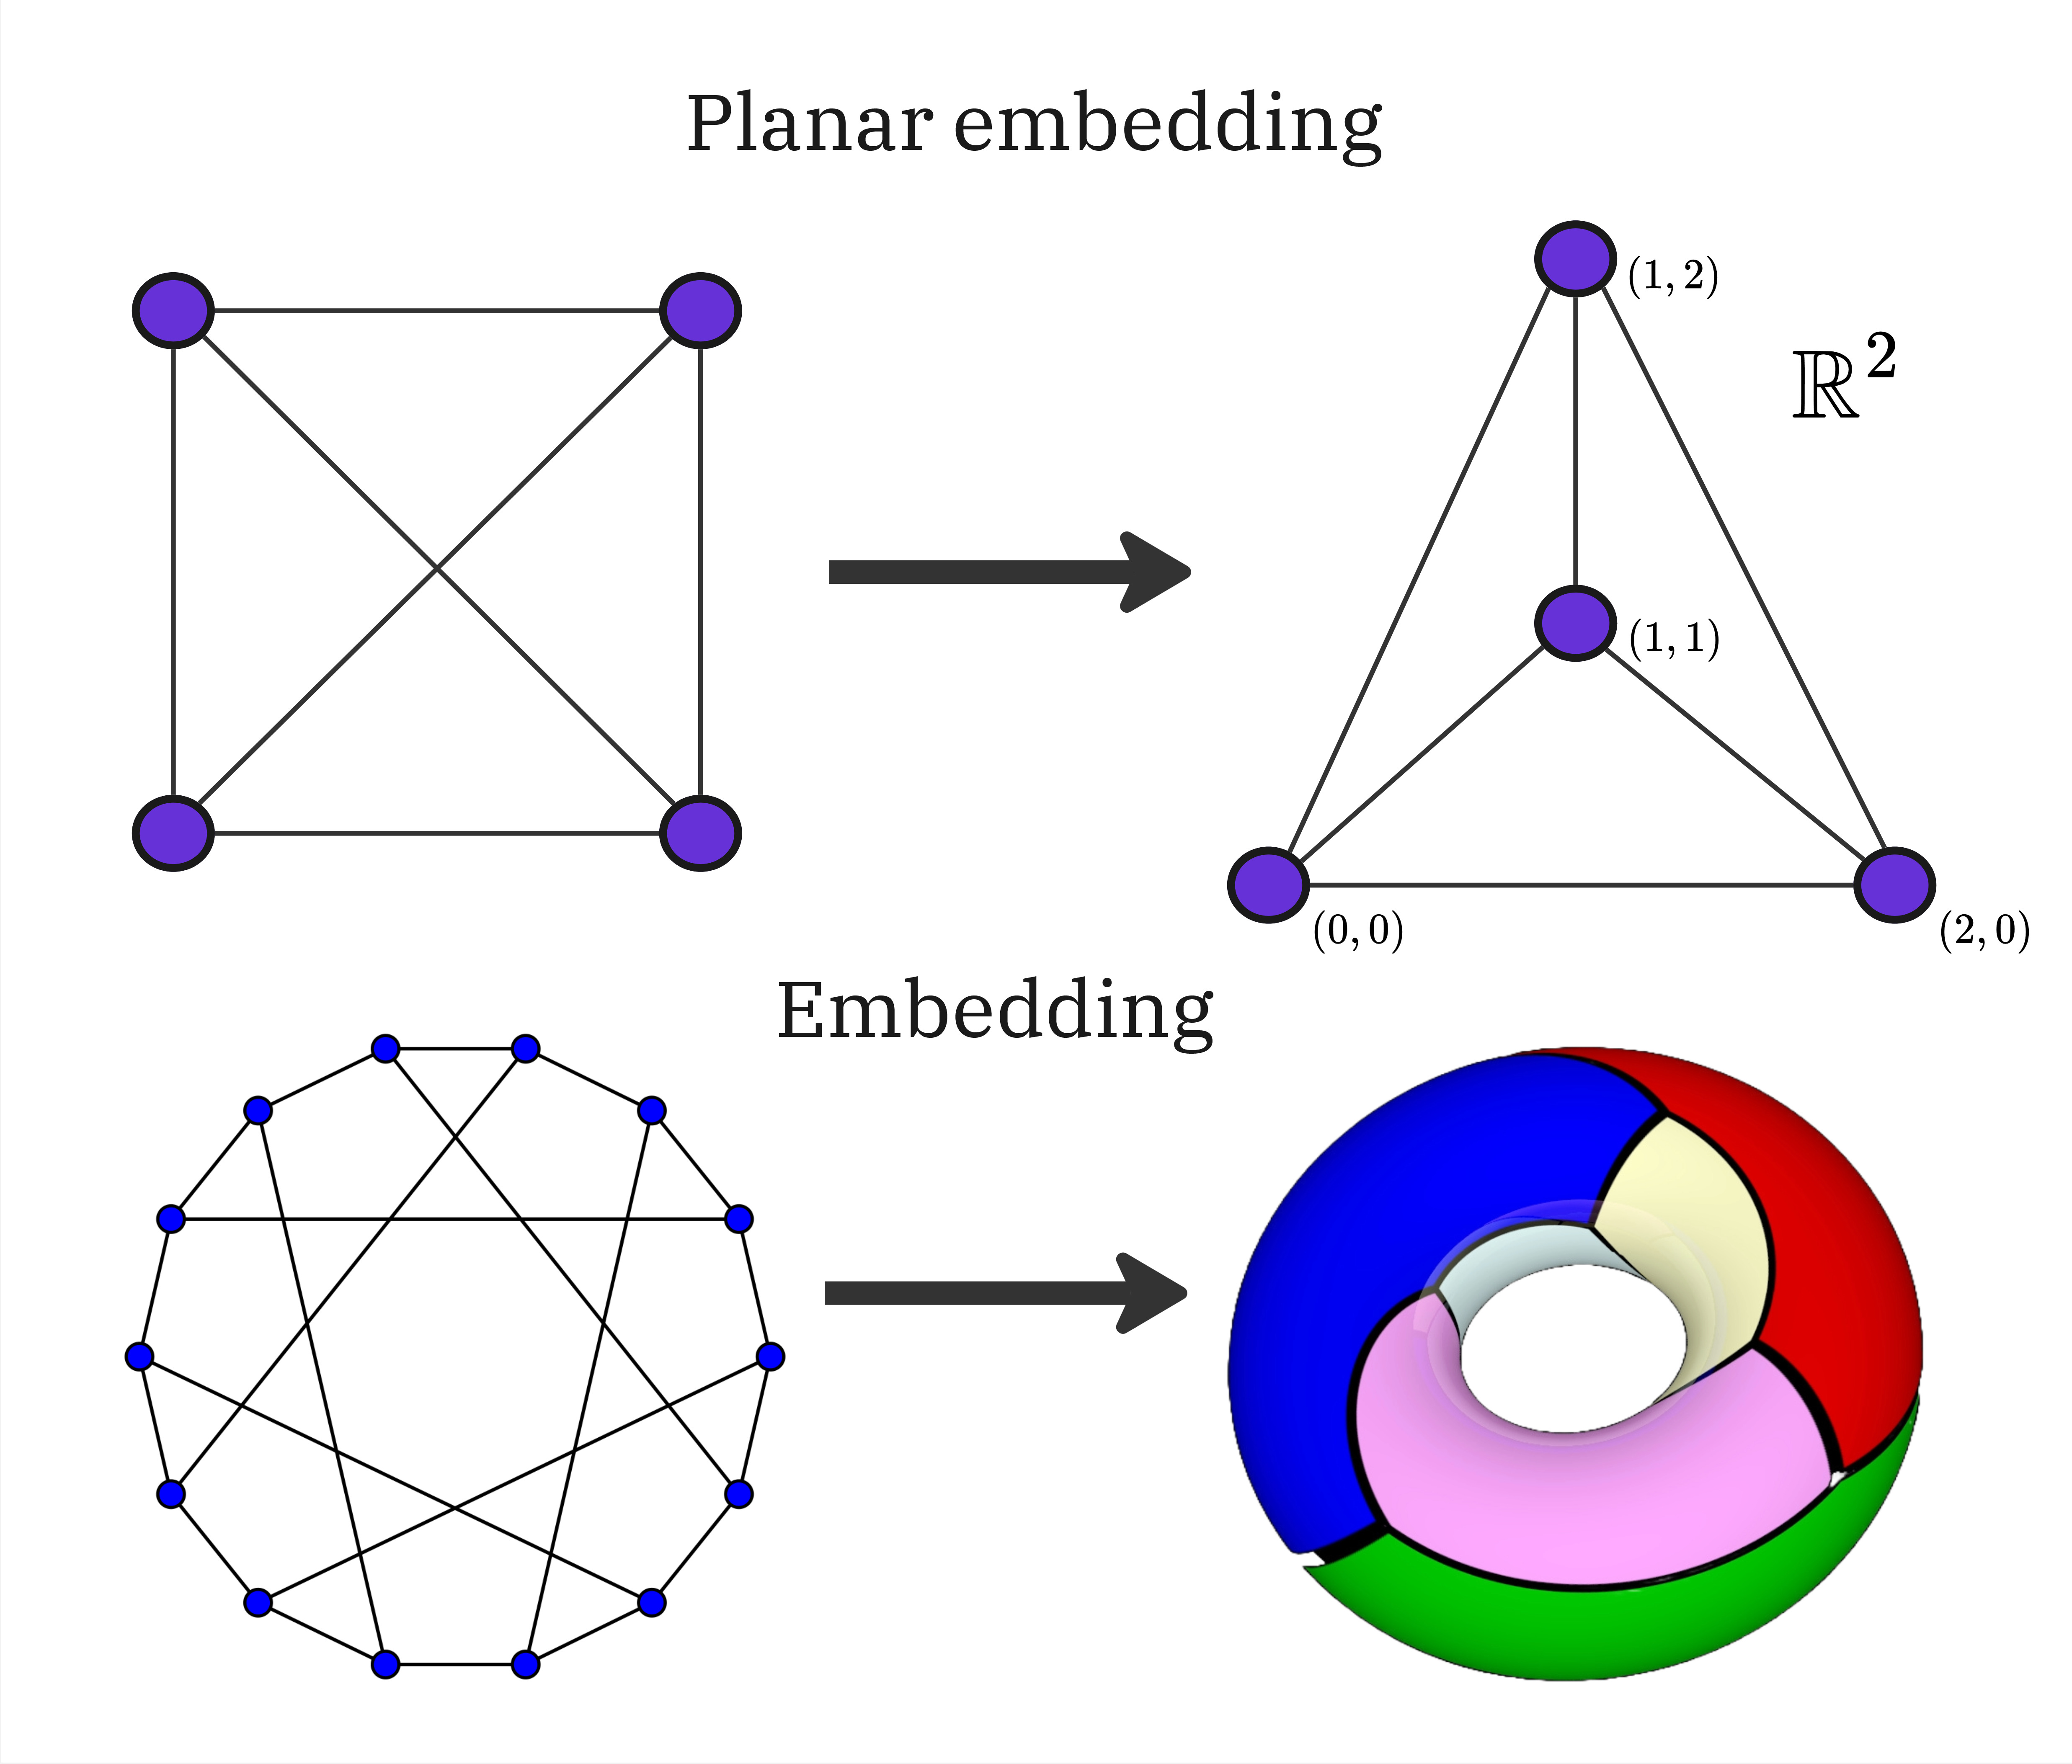
\includegraphics[height=8cm]{images/embedding.jpg}
    \end{minipage}
\end{frame}

\begin{frame}{Muito Mais Definições}
    \centering
    \large
    Um grafo é \textbf{\emph{outerplanar}} se admite uma imersão planar com todos os vértices na face externa.
    \bigbreak
    \begin{minipage}{\linewidth}
        \centering
        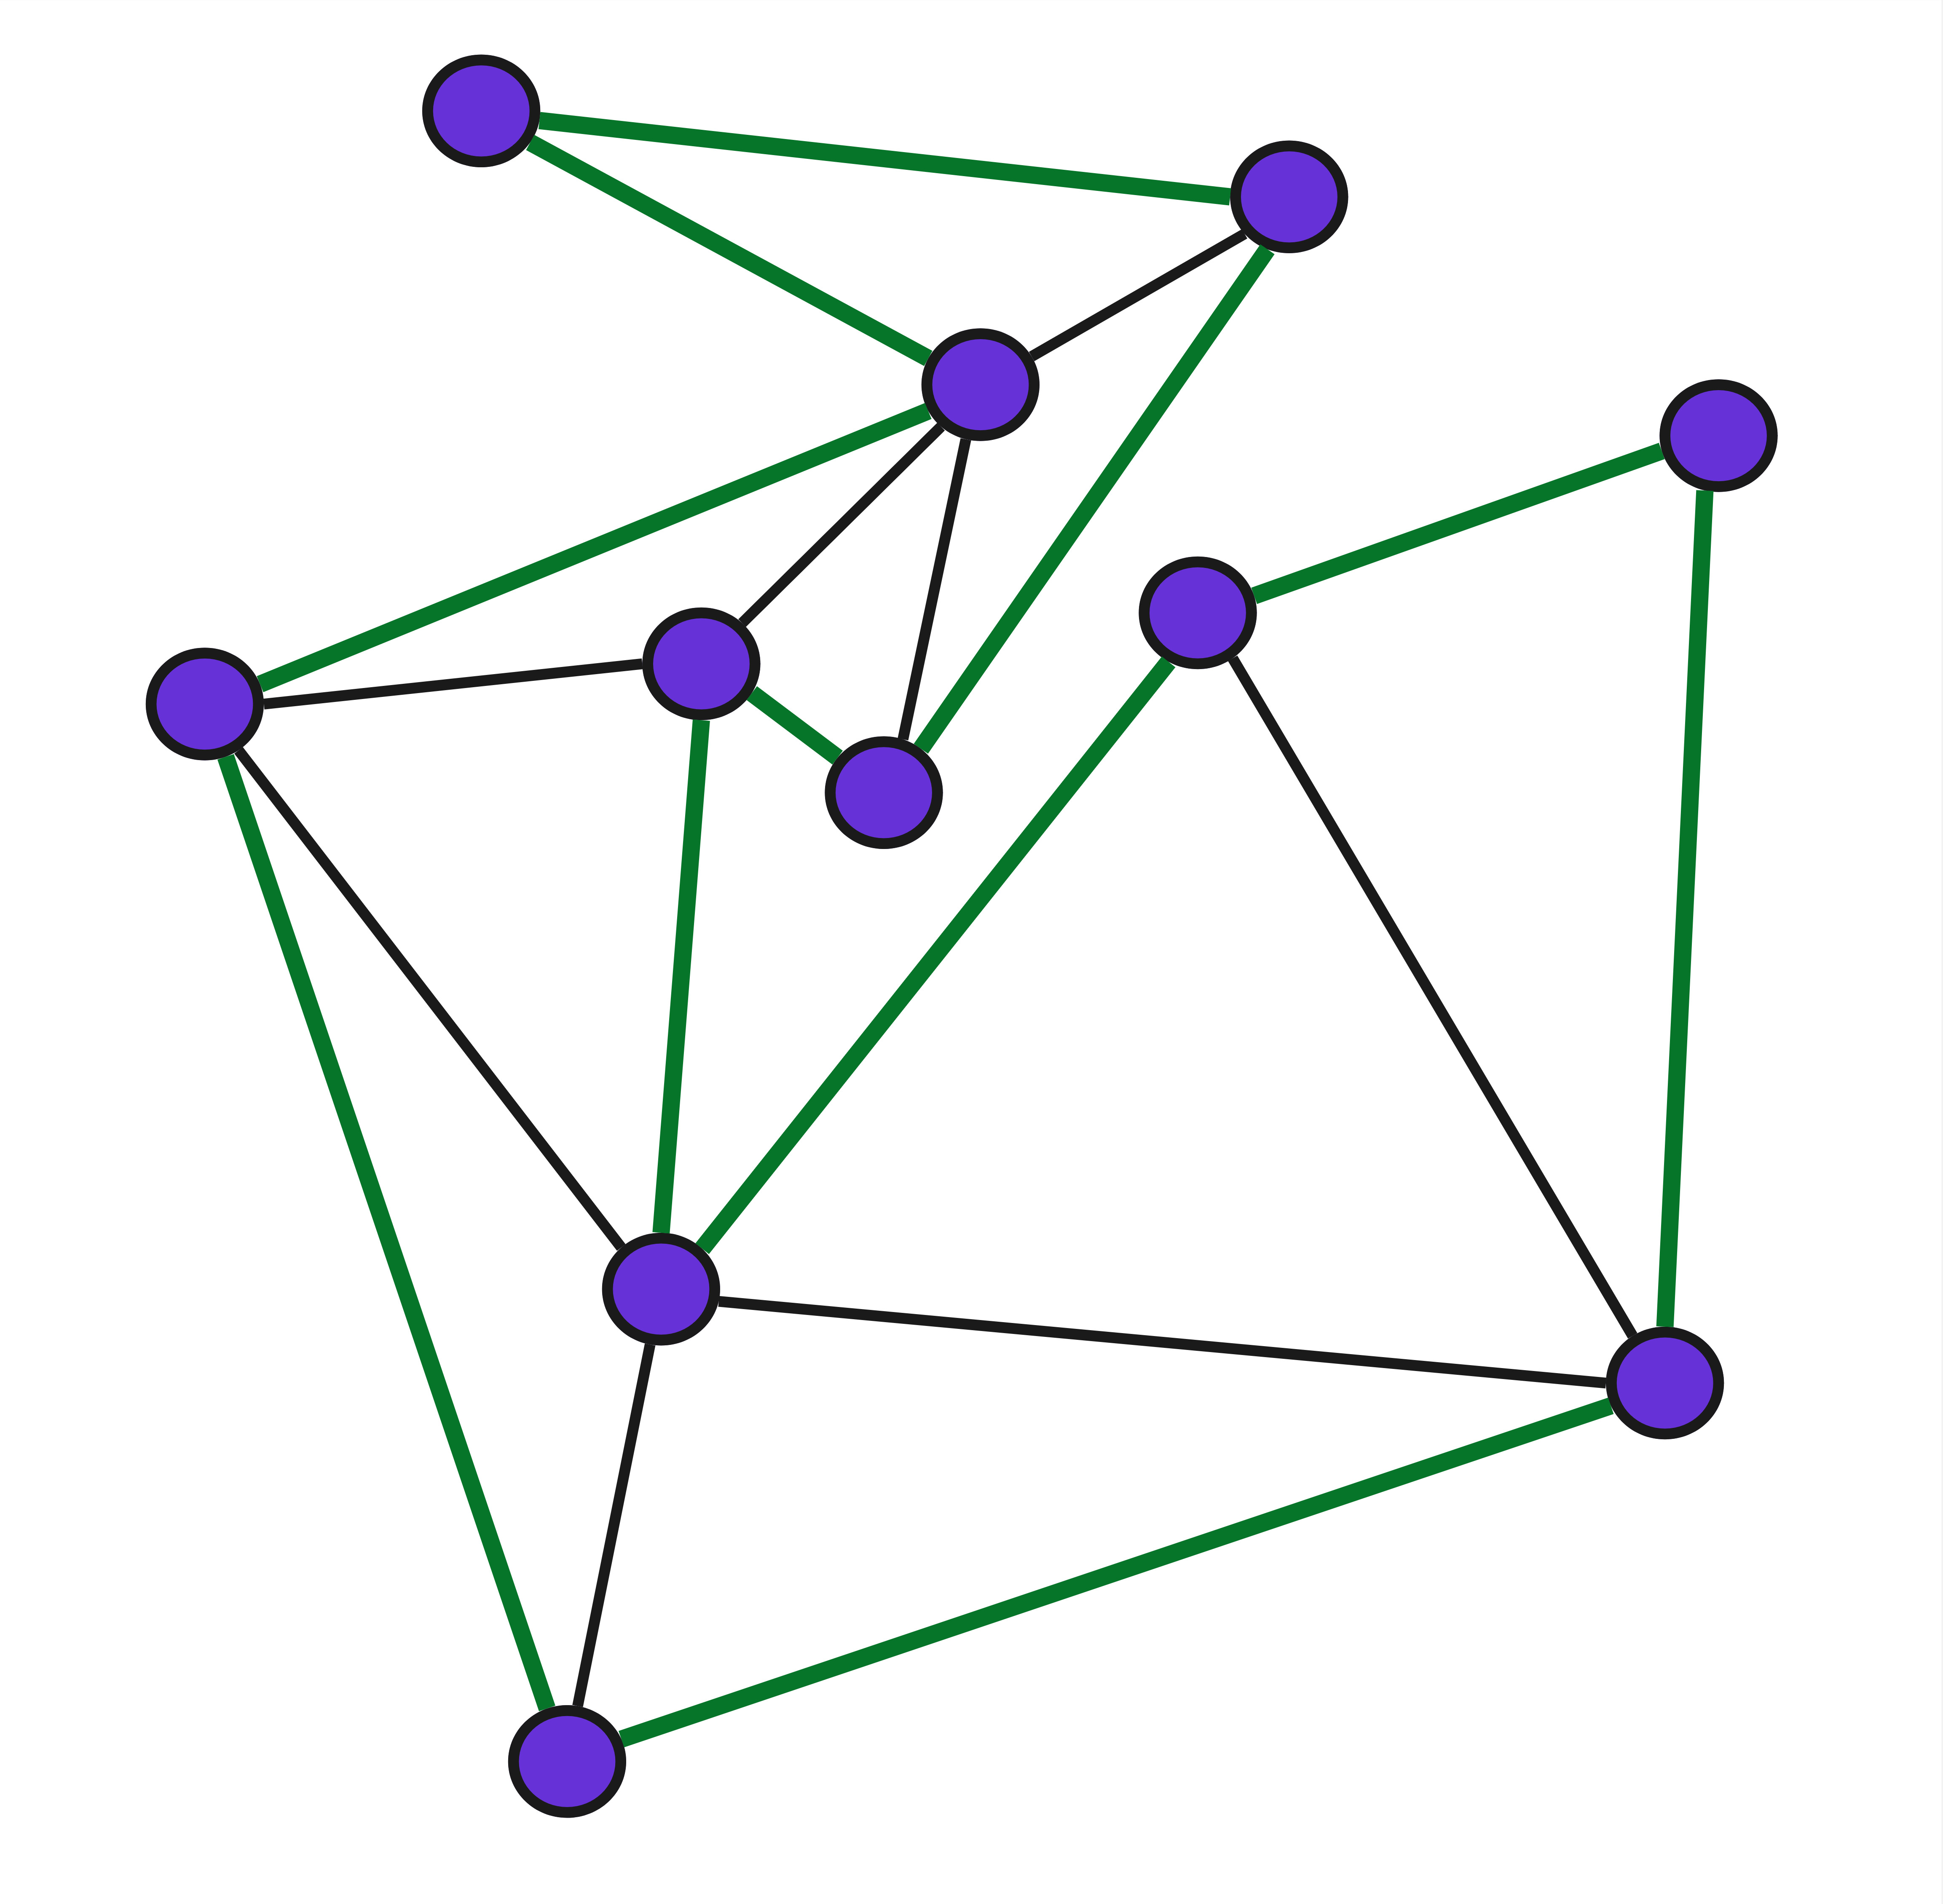
\includegraphics[height=3cm]{images/outerplanar.jpg}
    \end{minipage}
    \pause\bigbreak
    Todo grafo planar é outerplanar?\\
    \pause
    Não! Considere o $K_4$
    \bigbreak
    \begin{minipage}{\linewidth}
        \centering
        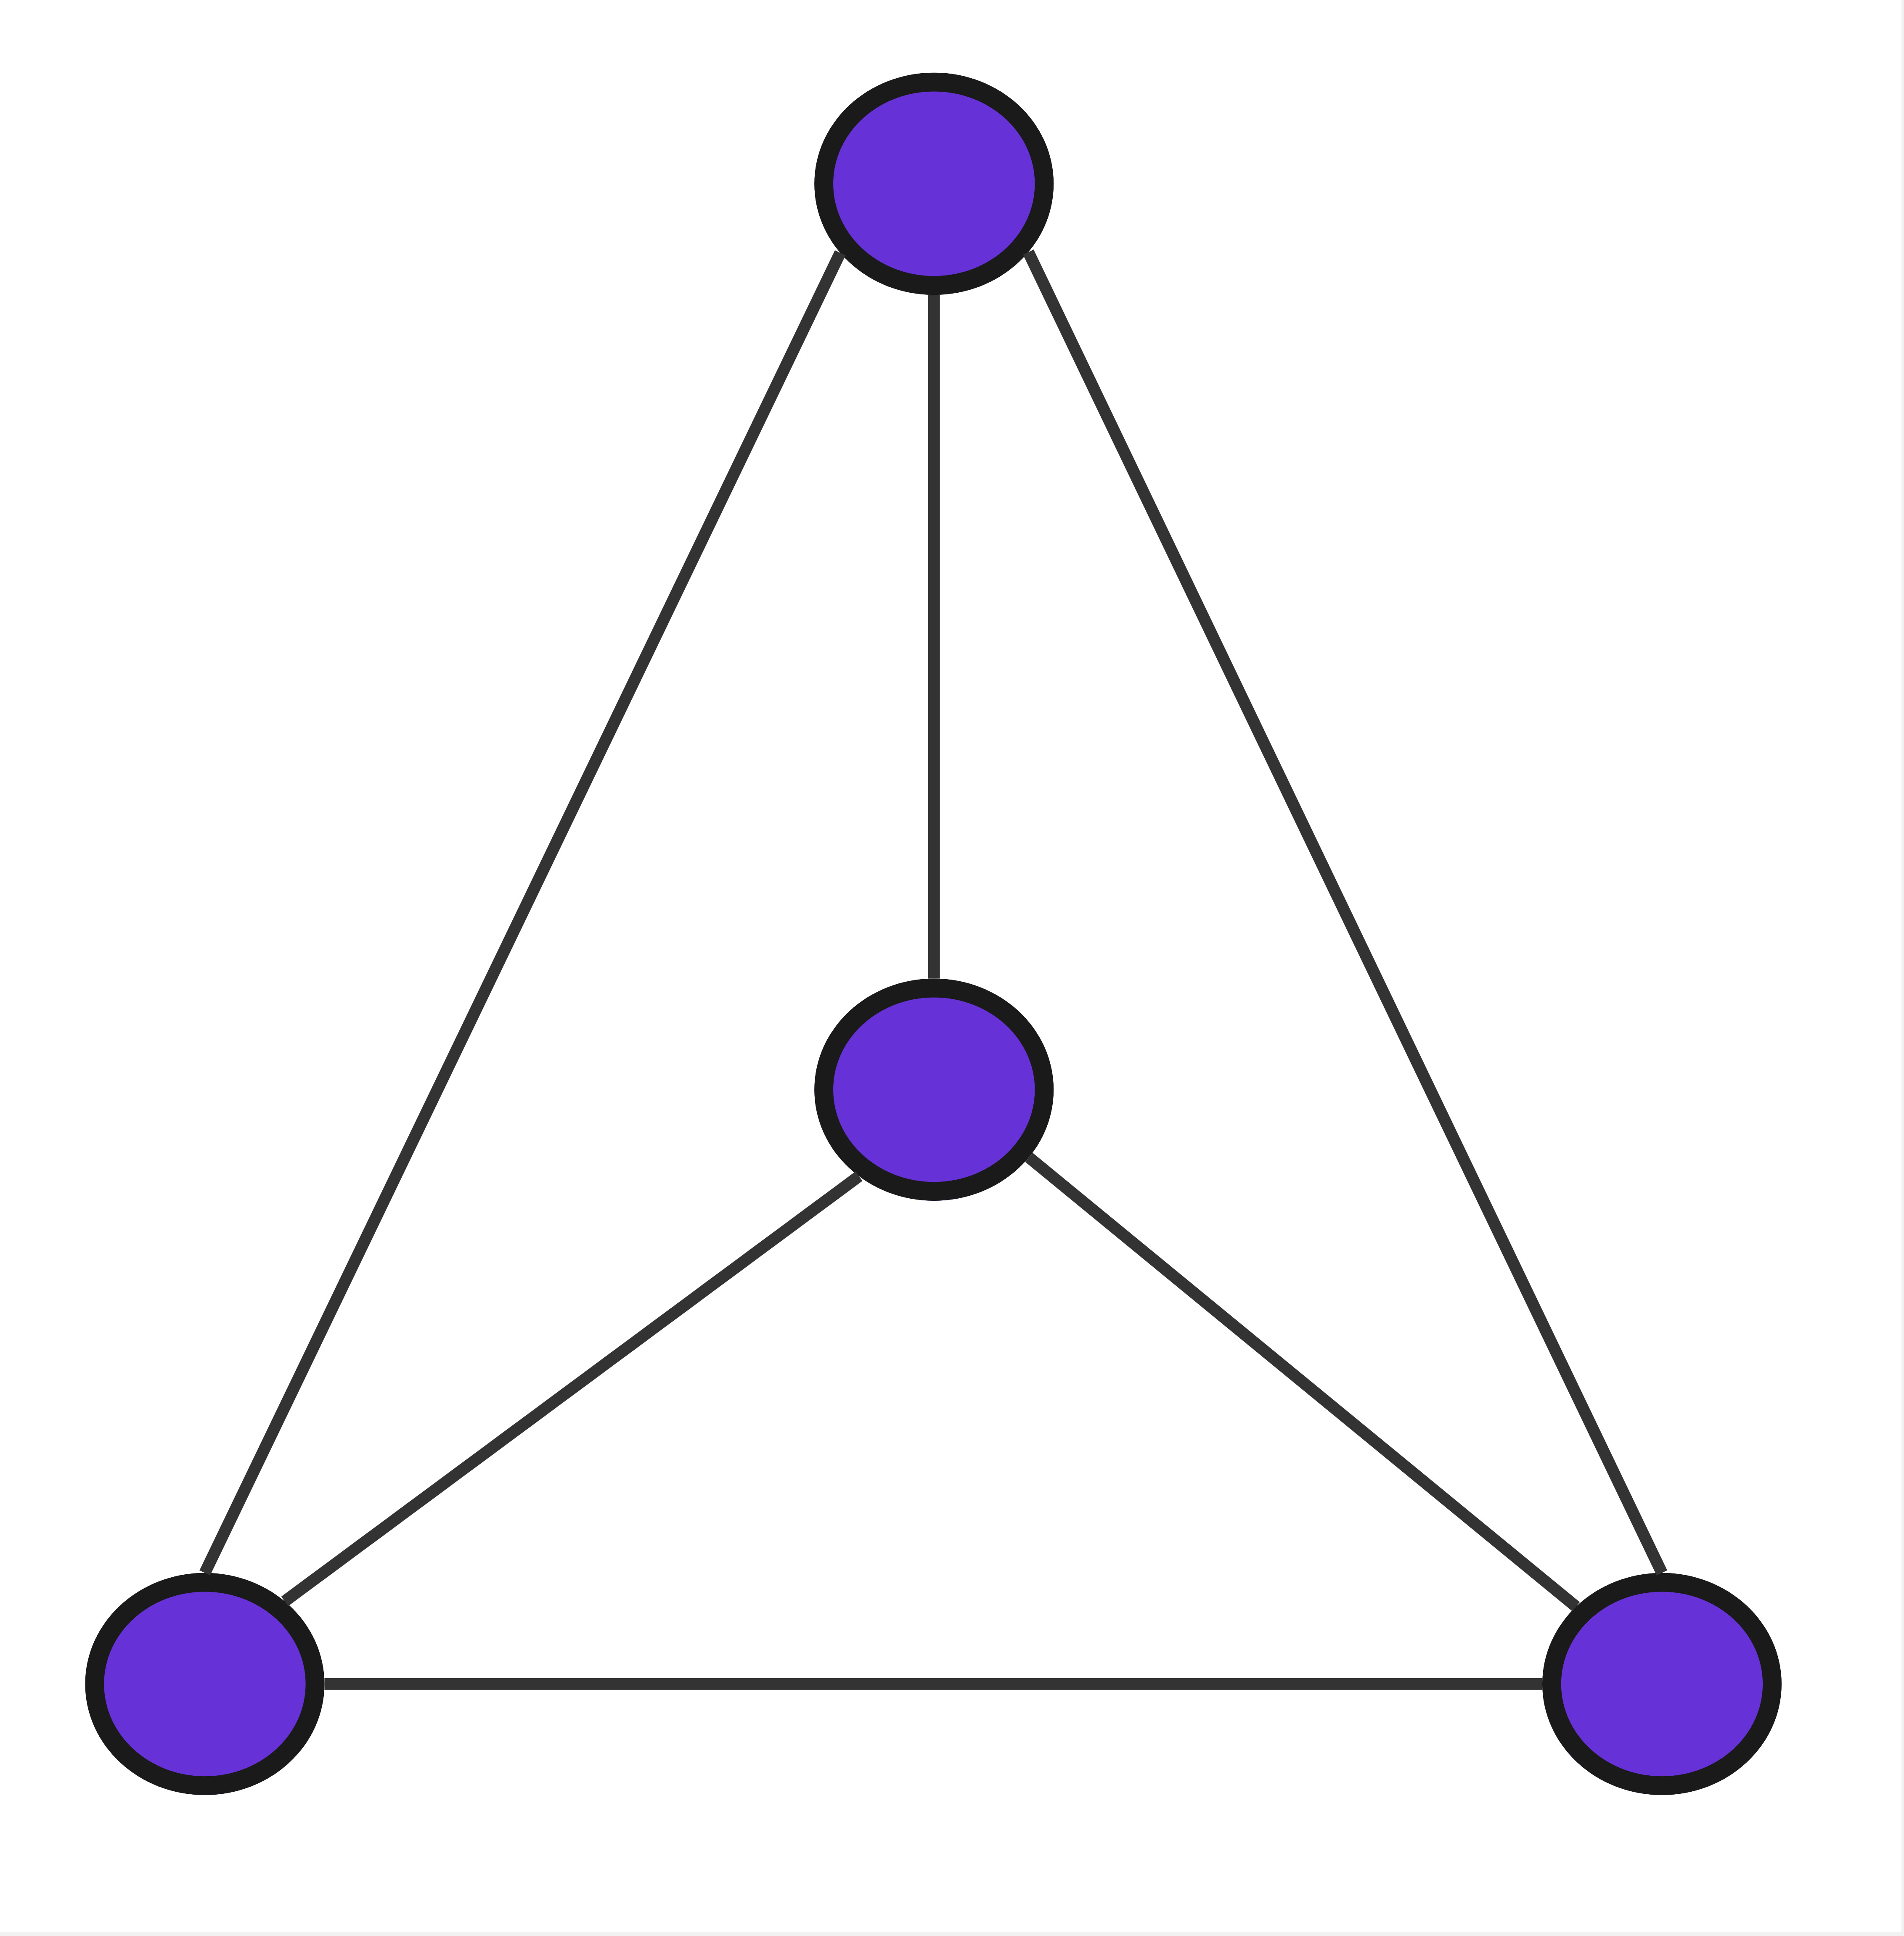
\includegraphics[height=2cm]{images/k4_graph.jpg}
    \end{minipage}
\end{frame}

\begin{frame}{Ainda Mais Definições}
    \centering
    \LARGE
    Nível 1
    \bigbreak
    \begin{minipage}{\linewidth}
        \centering
        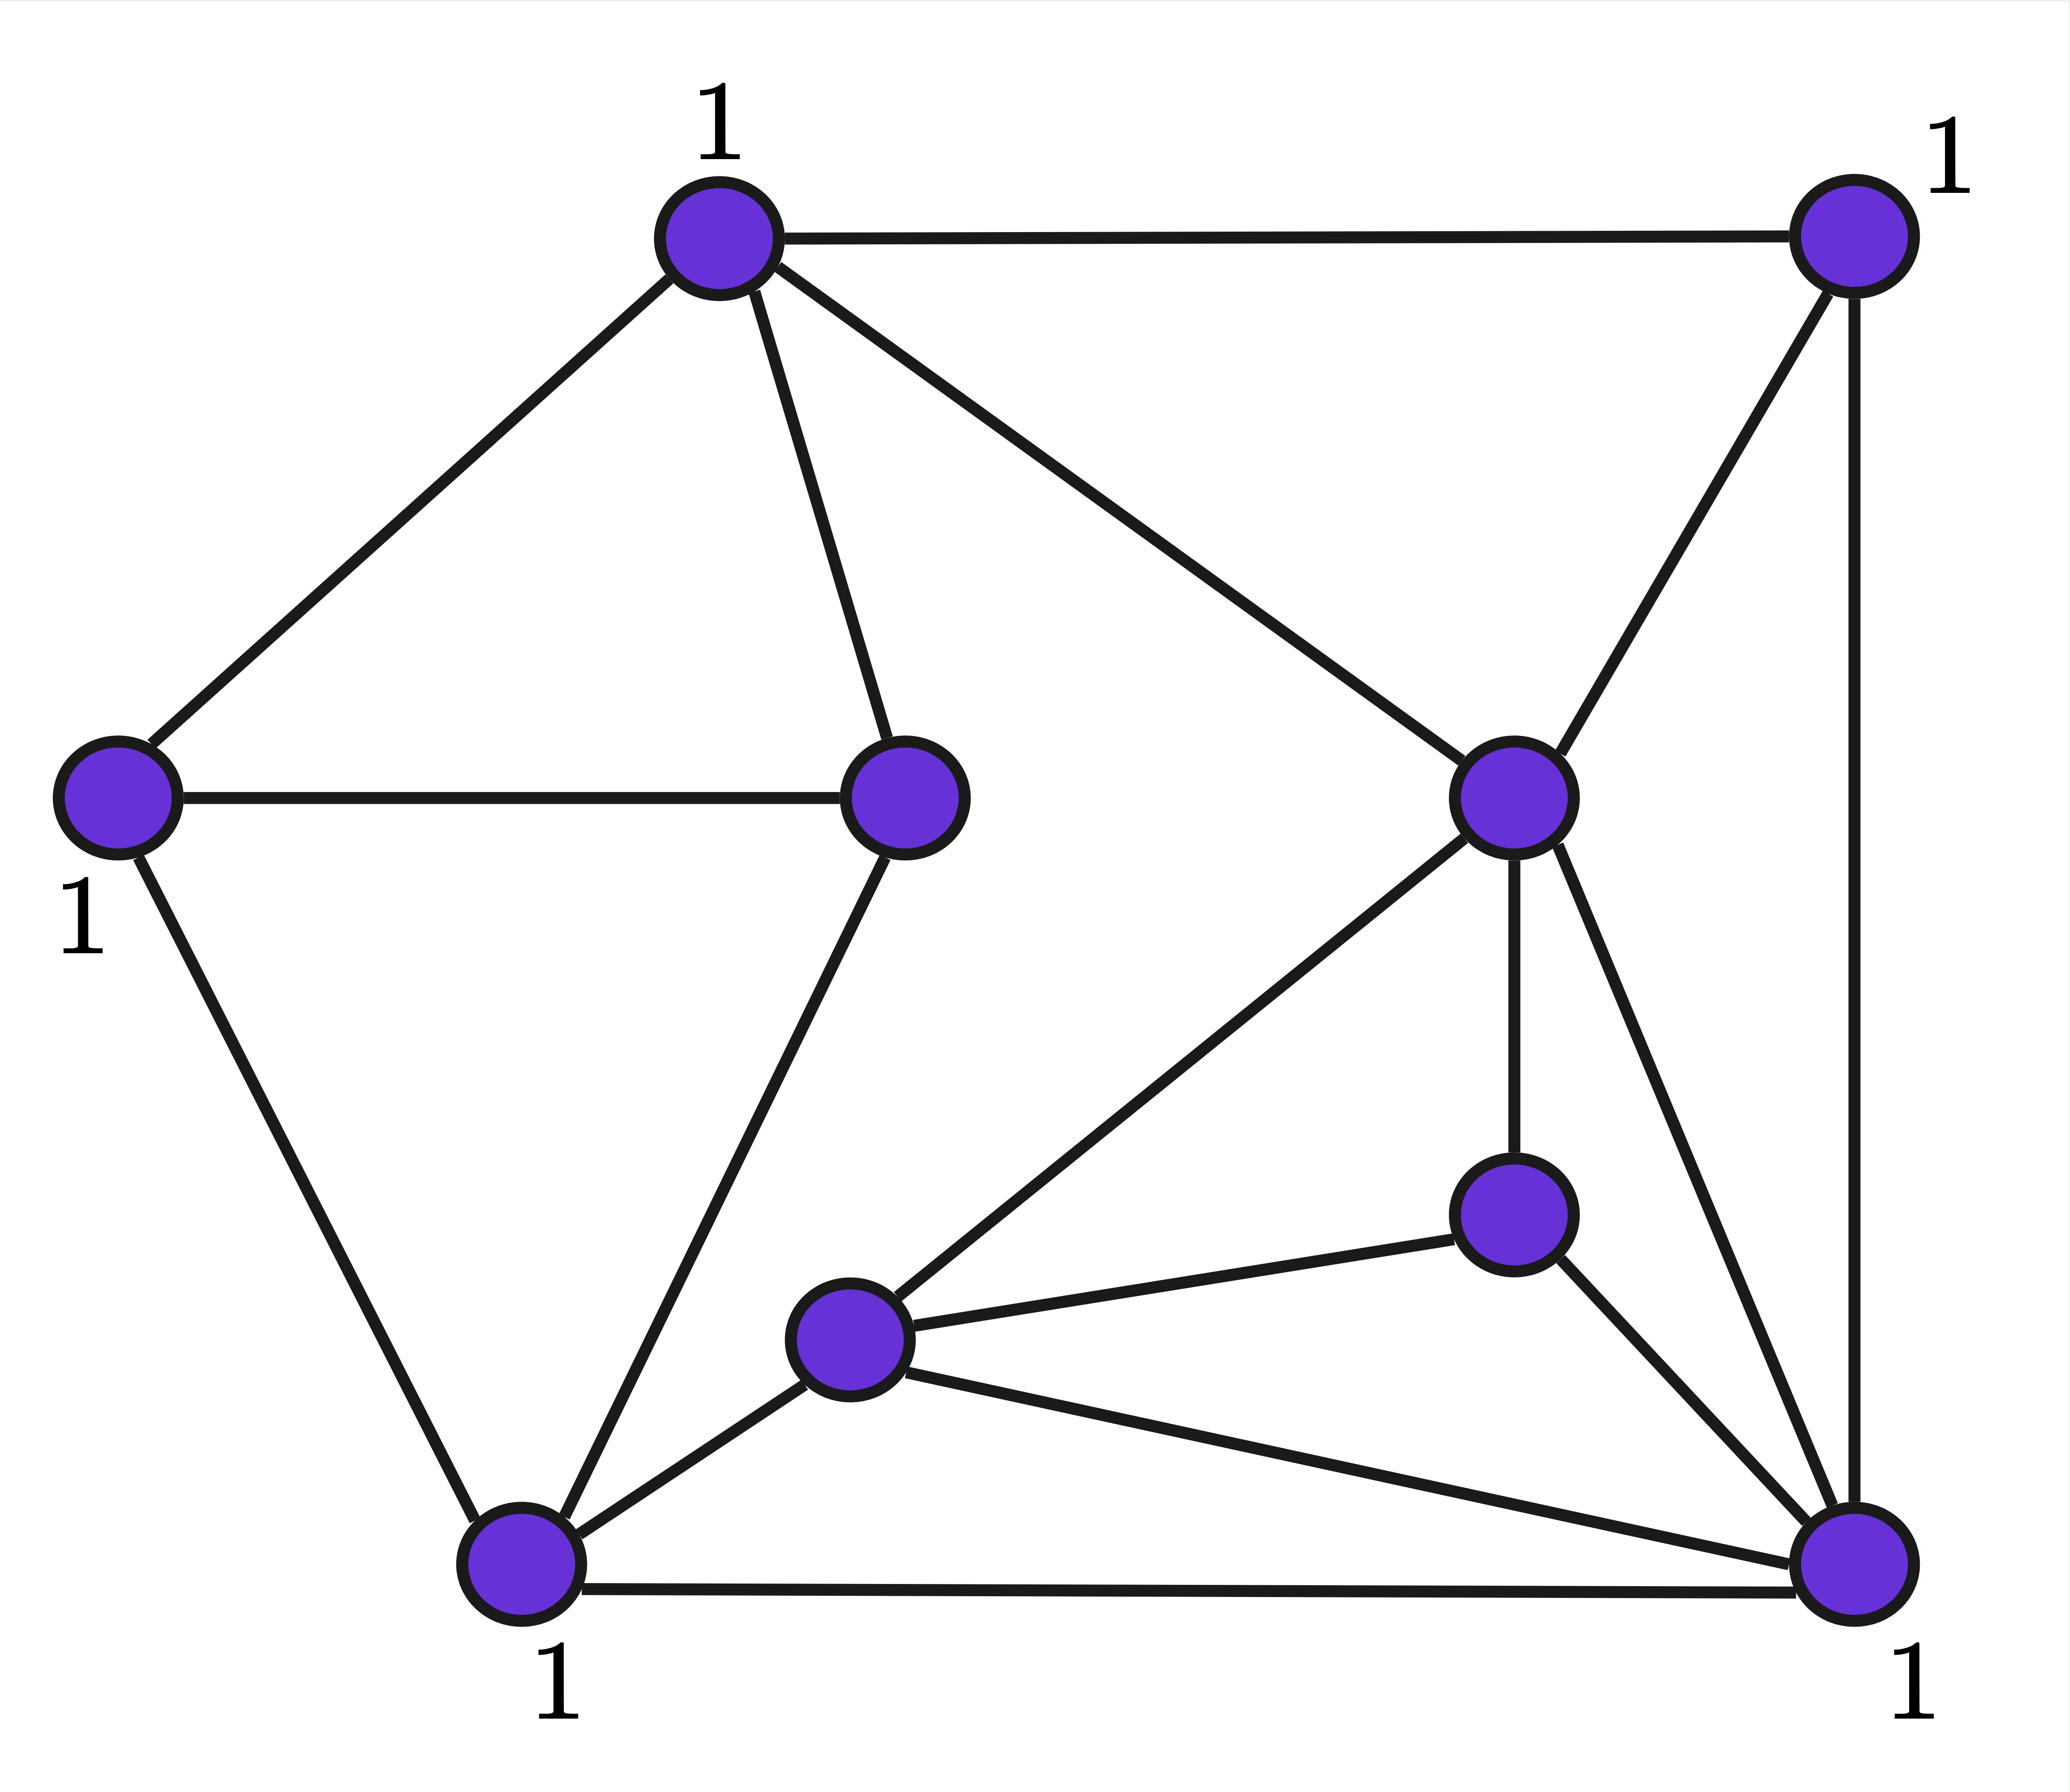
\includegraphics[height=5cm]{images/k_outerplanar_1.jpg}
    \end{minipage}
\end{frame}

\begin{frame}{Ainda Mais Definições}
    \centering
    \LARGE
    Nível 1 e Nível 2
    \begin{minipage}{\linewidth}
        \centering
        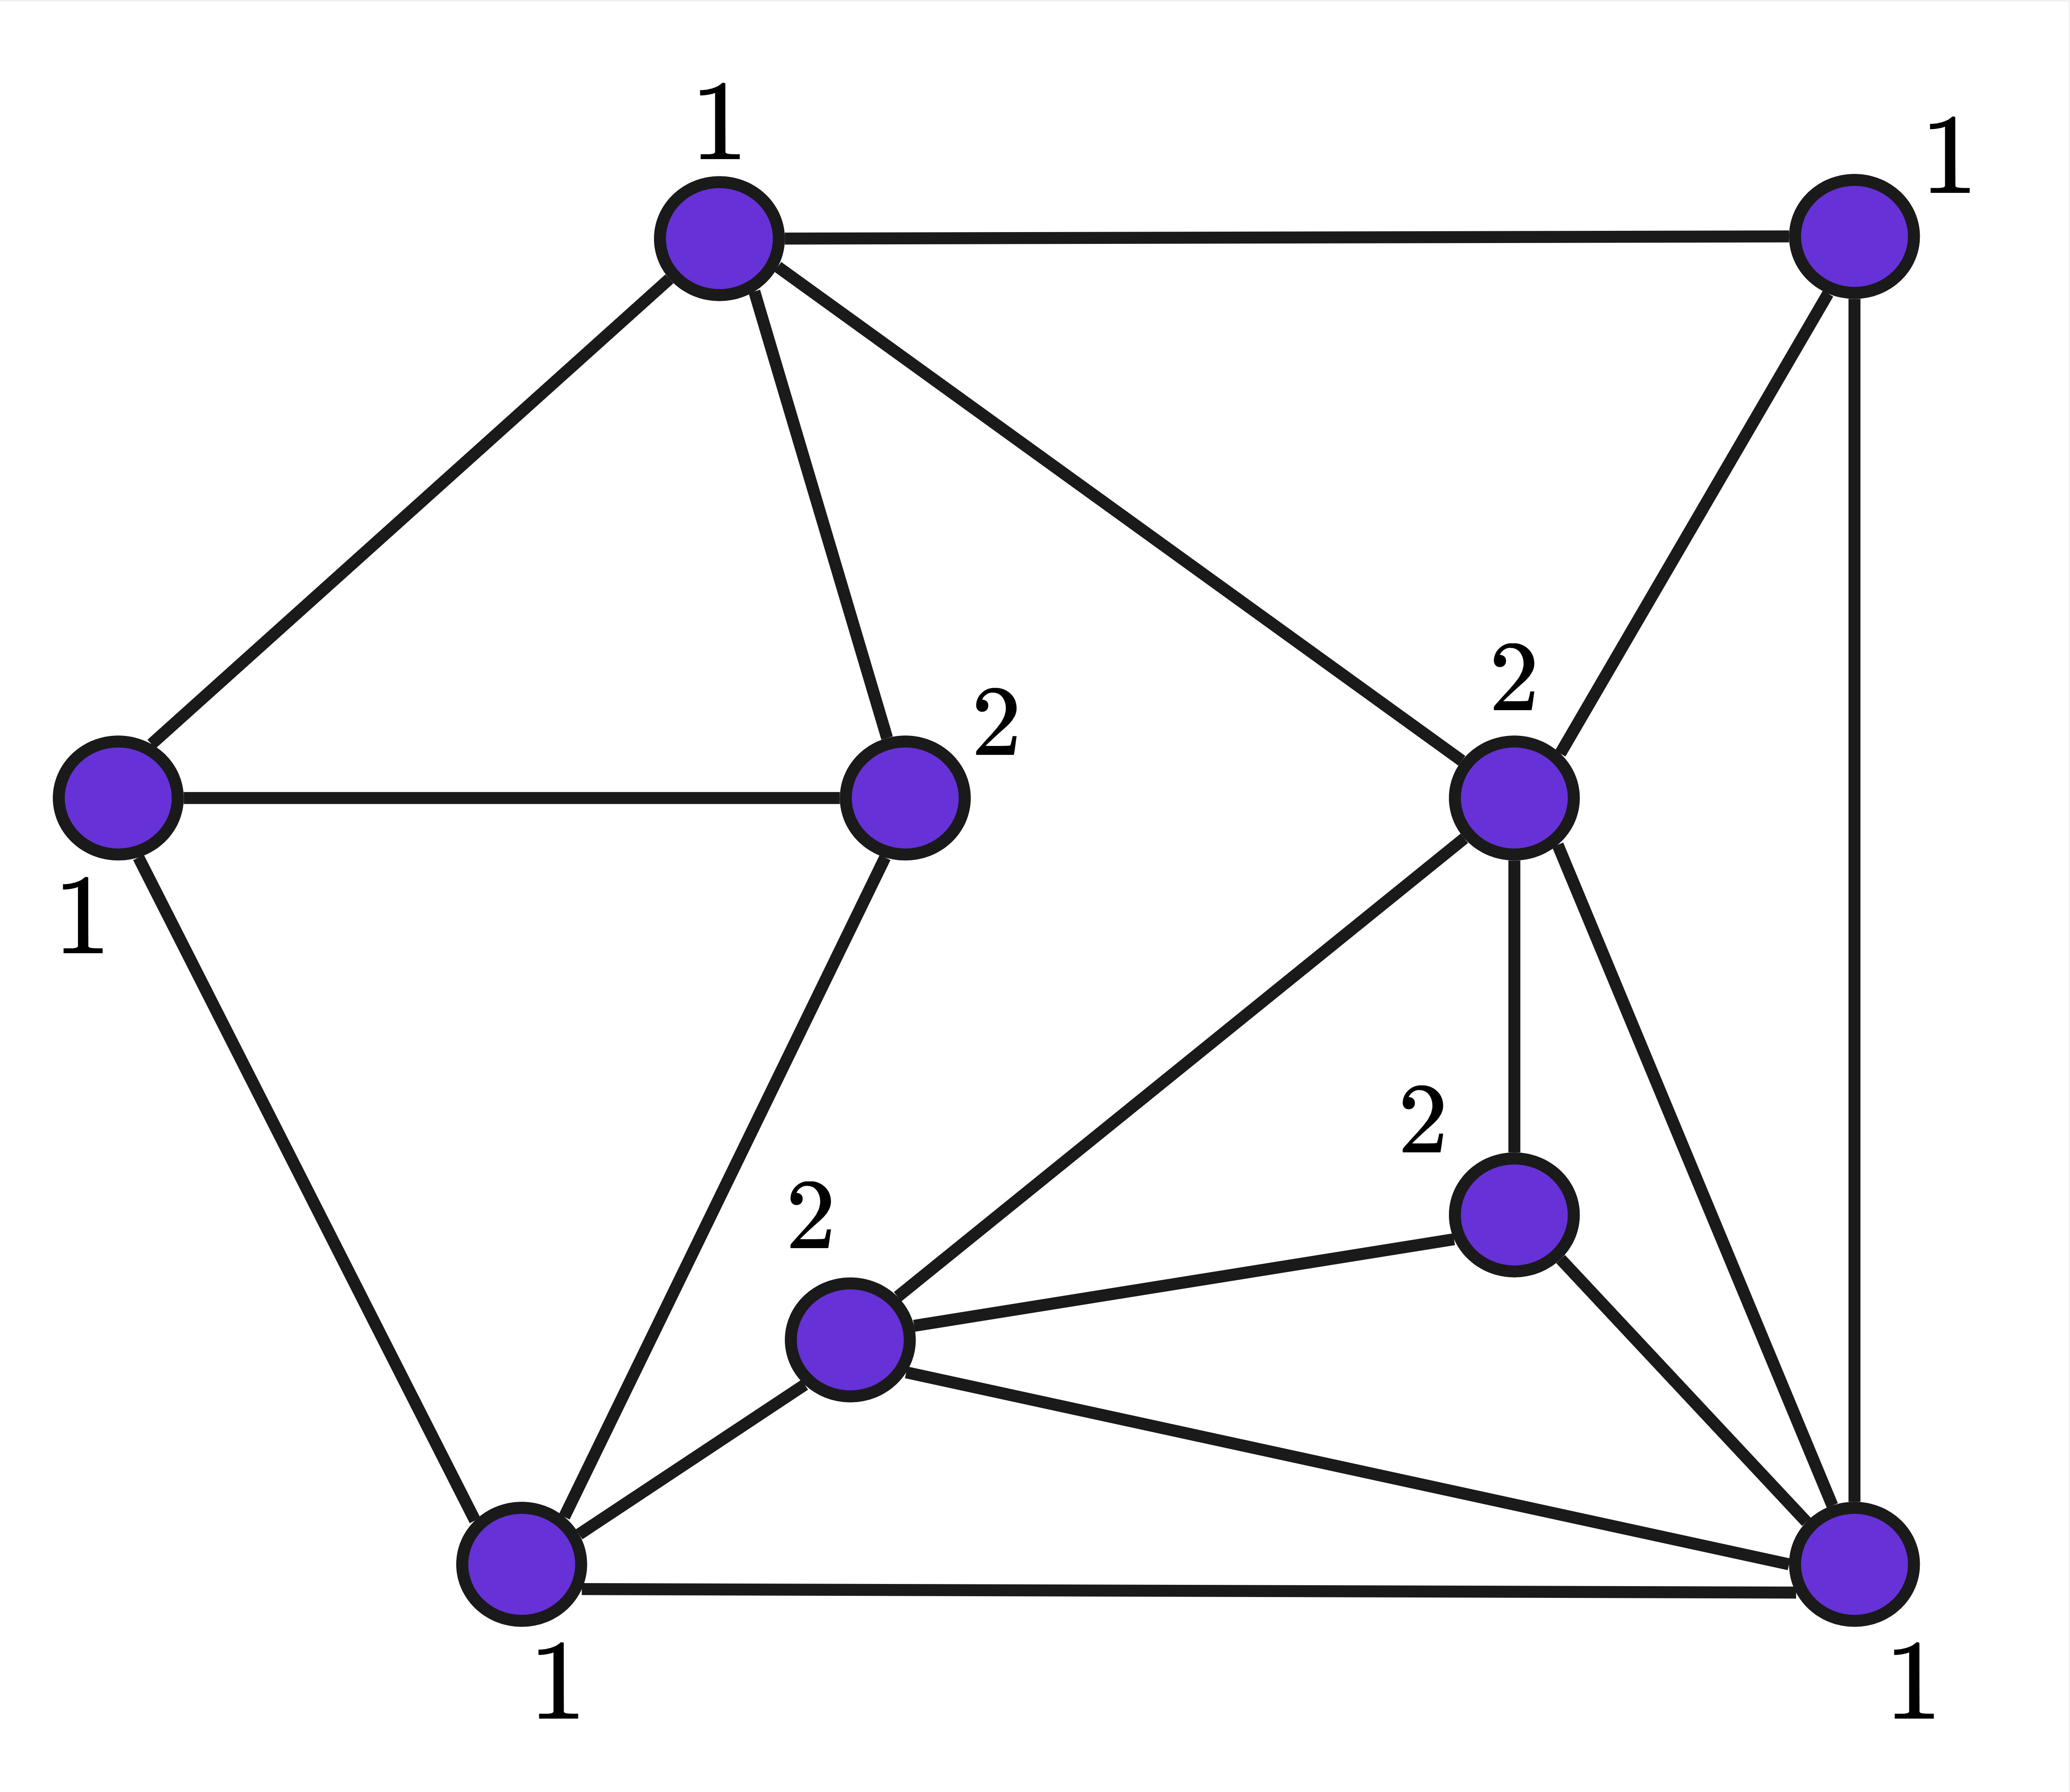
\includegraphics[height=5cm]{images/k_outerplanar_2.jpg}
    \end{minipage}
\end{frame}

\begin{frame}{Ainda Mais Definições}
    \centering
    \LARGE
    Nível 1, Nível 2 e Nível 3
    \begin{minipage}{\linewidth}
        \centering
        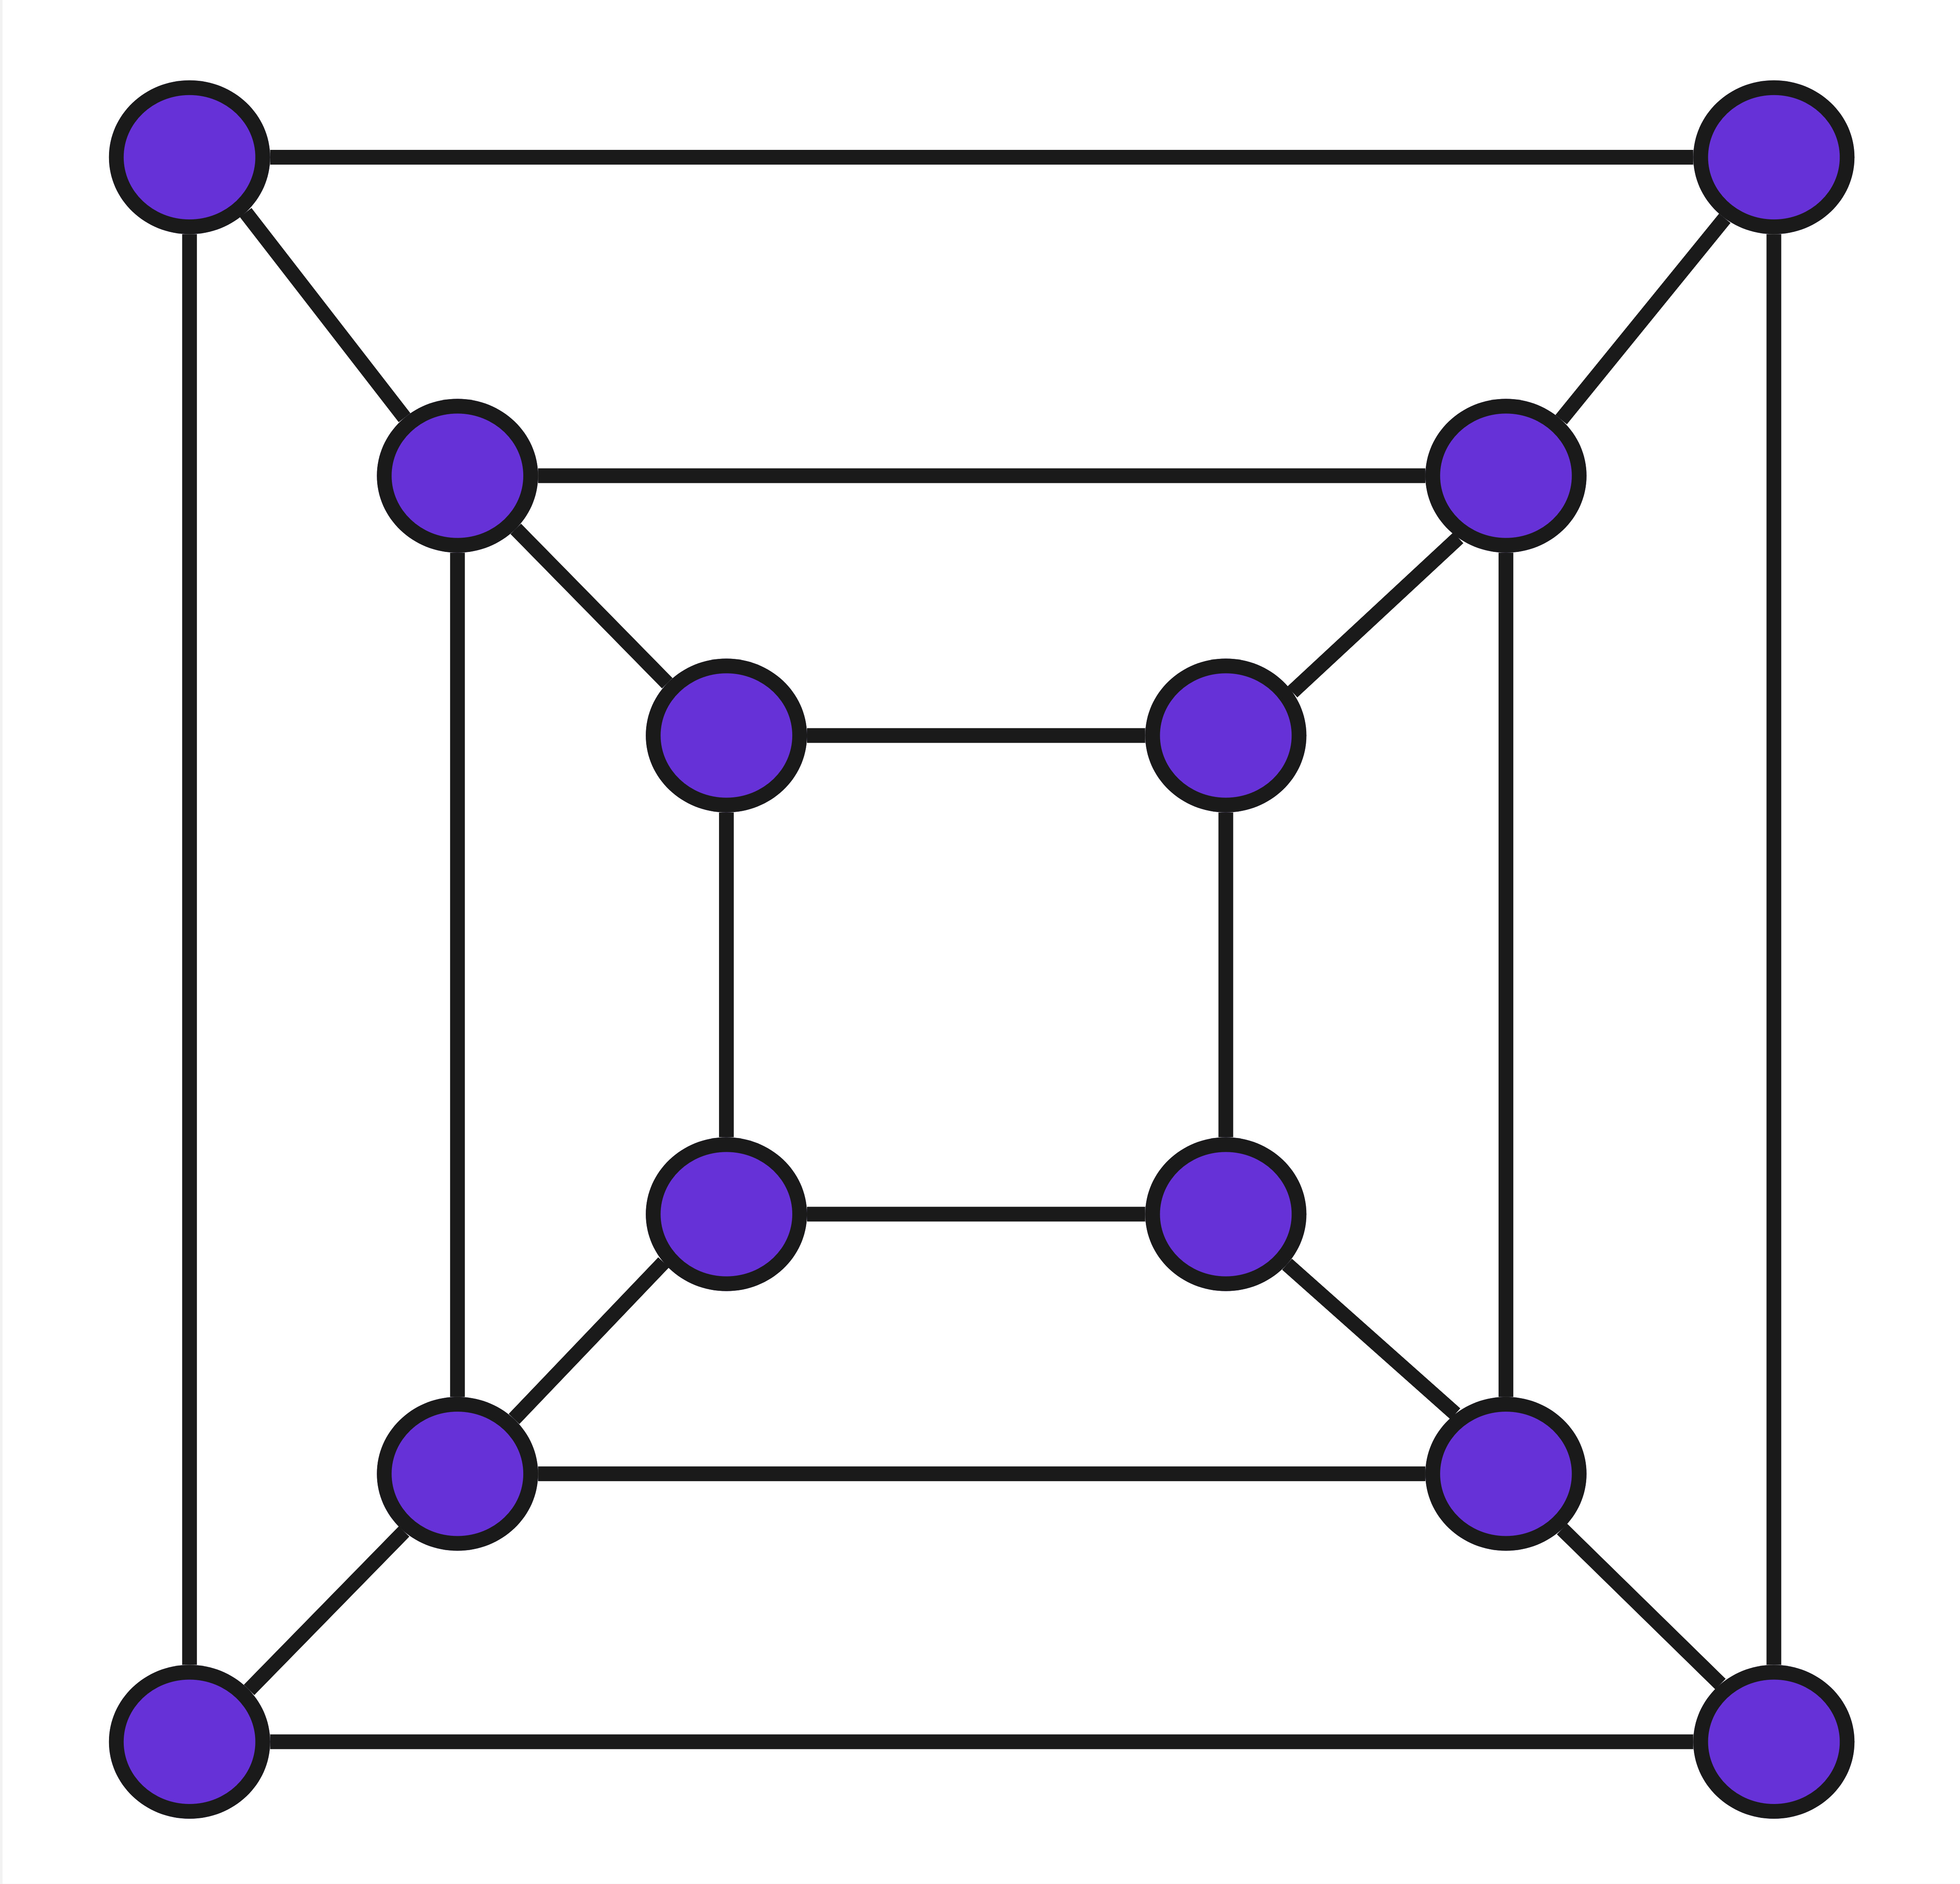
\includegraphics[height=5cm]{images/k_outerplanar_3.jpg}
    \end{minipage}
\end{frame}

\begin{frame}{Quando as Definições Vão Acabar!?}
    \begin{block}{Observação}
        Os vértices de nível $i$ de uma imersão planar de $G$ são aqueles que estão na face externa após a remoção dos vértices de níveis $1, \dots, i-1$ e suas arestas incidentes.
    \end{block}
    \bigbreak
    \begin{block}{Definição}
        Um grafo $G$ é \textbf{\emph{$k$-outerplanar}} se admite uma imersão planar na qual todos os seus vértices pertencem a níveis de $1$ até $k$.
    \end{block}
\end{frame}


\section{Largura Arbórea dos $k$-outerplanar}
\begin{frame}{Roteiro}
    \textbf{Objetivo:} Limitar a largura arbórea de grafos $k$-outerplanar.\\
    \pause\bigbreak
    \textbf{Plano:}\\
    \vspace{0.2cm}
    \hspace{0.4cm}\textbf{Passo 1}: Considerar apenas grafos $k$-outerplanar de grau máximo $3$\\
    \pause
    \vspace{0.1cm}
    \hspace{0.4cm}\textbf{Passo 2}: Provar que grafos $k$-outerplanar de grau máximo três têm carga máxima limitada\\
    \pause
    \vspace{0.1cm}
    \hspace{0.4cm}\textbf{Passo 3}: Provar que carga máxima limitada implica em largura arbórea limitada
\end{frame}

\begin{frame}{Passo 1}
    \begin{lema}
        Todo grafo $k$-outerplanar $G$ pode ser transformado em um grafo $k$-outerplanar $G^{\prime}$ de grau máximo 3, tal que uma decomposição em árvore de $G^{\prime}$ corresponde a uma de $G$ de mesma largura.
    \end{lema}
    \begin{proof}
        Divida qualquer vértice $v$ de grau $d$ maior que $3$ em dois vértices $v_1, v_2$ de grau $3$ e $d-1$.\\
        \vspace{0.2cm}
        \begin{minipage}{\linewidth}
            \centering
            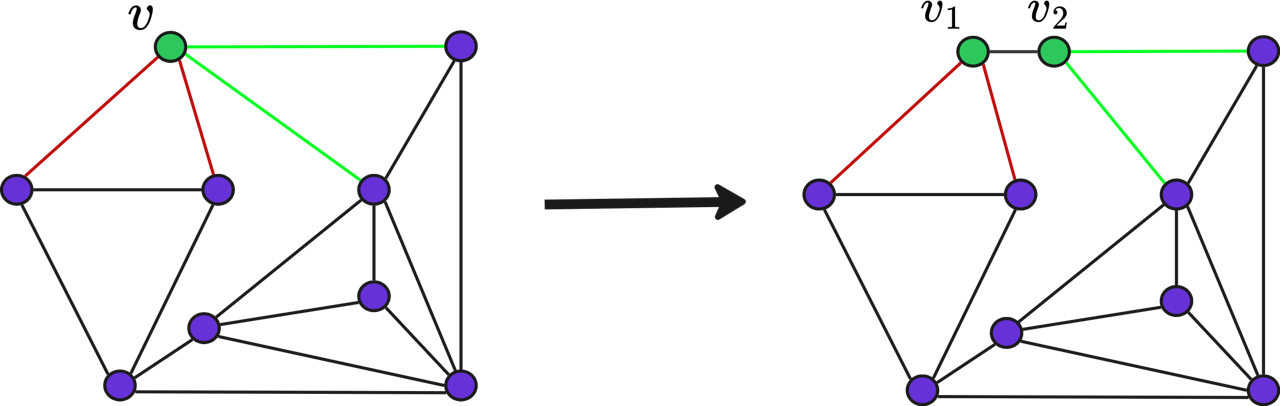
\includegraphics[width=6cm]{images/proof_1_1.png}
        \end{minipage}\\
        \vspace{0.4cm}
        Se $v_{1}$ ou $v_{2}$ estão em $X^{\prime}_{i}$, definimos $X_{i}=\{X^{\prime}_{i}\setminus\{v_{1}, v_{2}\}\} \cup \{v\}$; senão $X_{i}=X^{\prime}_{i}$. \phantom{\qedhere}
    \end{proof}
\end{frame}

\begin{frame}{Passo 1\dots}
    \begin{proof}
        \begin{itemize}[-]
            \item Crie uma sequência de decomposições $G_{1}, G_{2}, \dots, G_{z}$ tal que $G_{z}$ tem grau máximo $3$;
            \item Obtenha uma decomposição em árvore de $G_z$;
            \item Construa decomposições para $G_{z-1}, G_{z-2}, \dots, G_1, G$, de tal forma que a decomposição final de $G$ tenha largura no máximo igual à de $G_z$.
        \end{itemize}
        \alt<4>{\qedhere}{\phantom\qedhere}
    \end{proof}
\end{frame}

\begin{frame}{Definições Que Nunca Acabam}
    \Large{Dada uma floresta geradora maximal $(V, F)$ de um grafo $G$, e uma aresta $e \in E \setminus F$:}
    \bigbreak

    \begin{defi}[Ciclo fundamental]
        O \emph{\textbf{ciclo fundamental}} de $e$ é o ciclo formado ao adicionar $e$ à $F$.
    \end{defi}
\end{frame}

\begin{frame}{Definições Que Nunca Acabam}
    \begin{defi}[Carga de vértice]
        A \emph{\textbf{carga de um vértice}} $v \in V$ é o número de ciclos fundamentais em que $v$ aparece.
    \end{defi}

    \begin{defi}[Carga aresta]
        A \emph{\textbf{carga de uma aresta}} $e \in F$ é o número de ciclos fundamentais que a contêm.
    \end{defi}
\end{frame}

\begin{frame}{Quiz}
    \centering\Large
    Encontre a carga do vértice e aresta vermelhos\bigbreak
    \begin{minipage}{\linewidth}
        \centering
        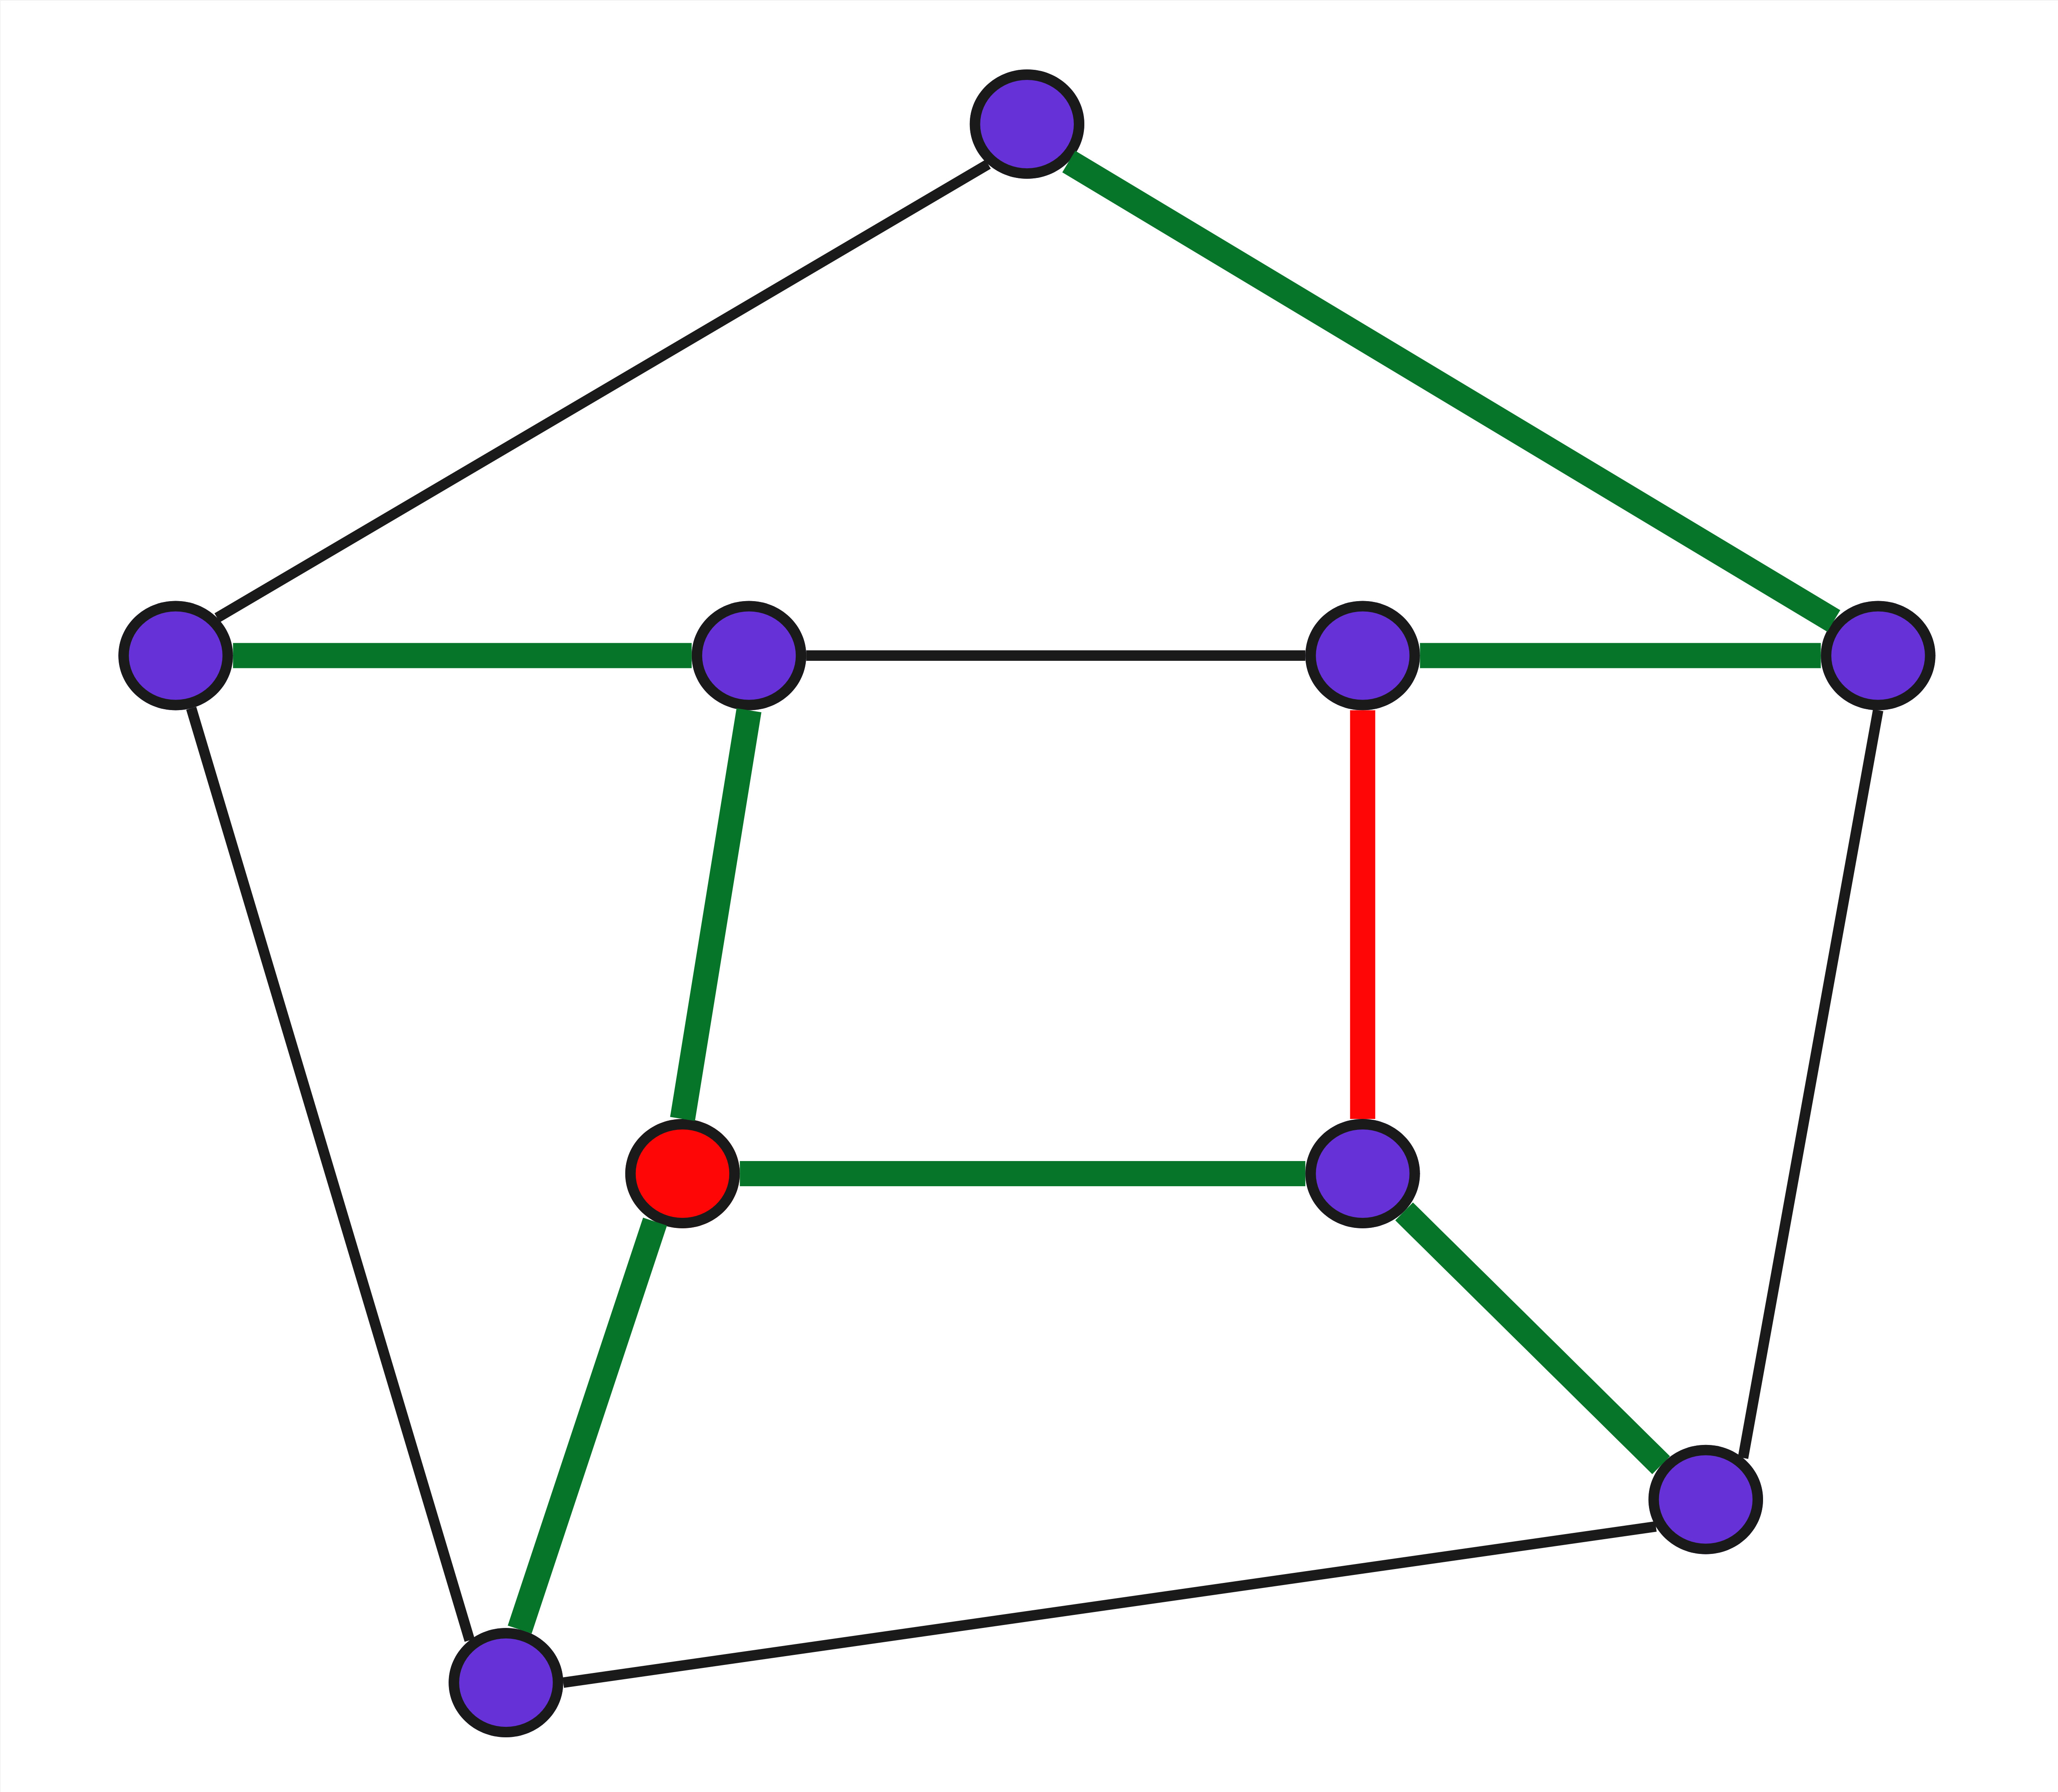
\includegraphics[width=7cm]{images/load_1.jpg}
    \end{minipage}
\end{frame}

\begin{frame}{Quiz}
    \centering\Large
    Encontre a carga do vértice e aresta vermelhos\bigbreak
    \begin{minipage}{\linewidth}
        \centering
        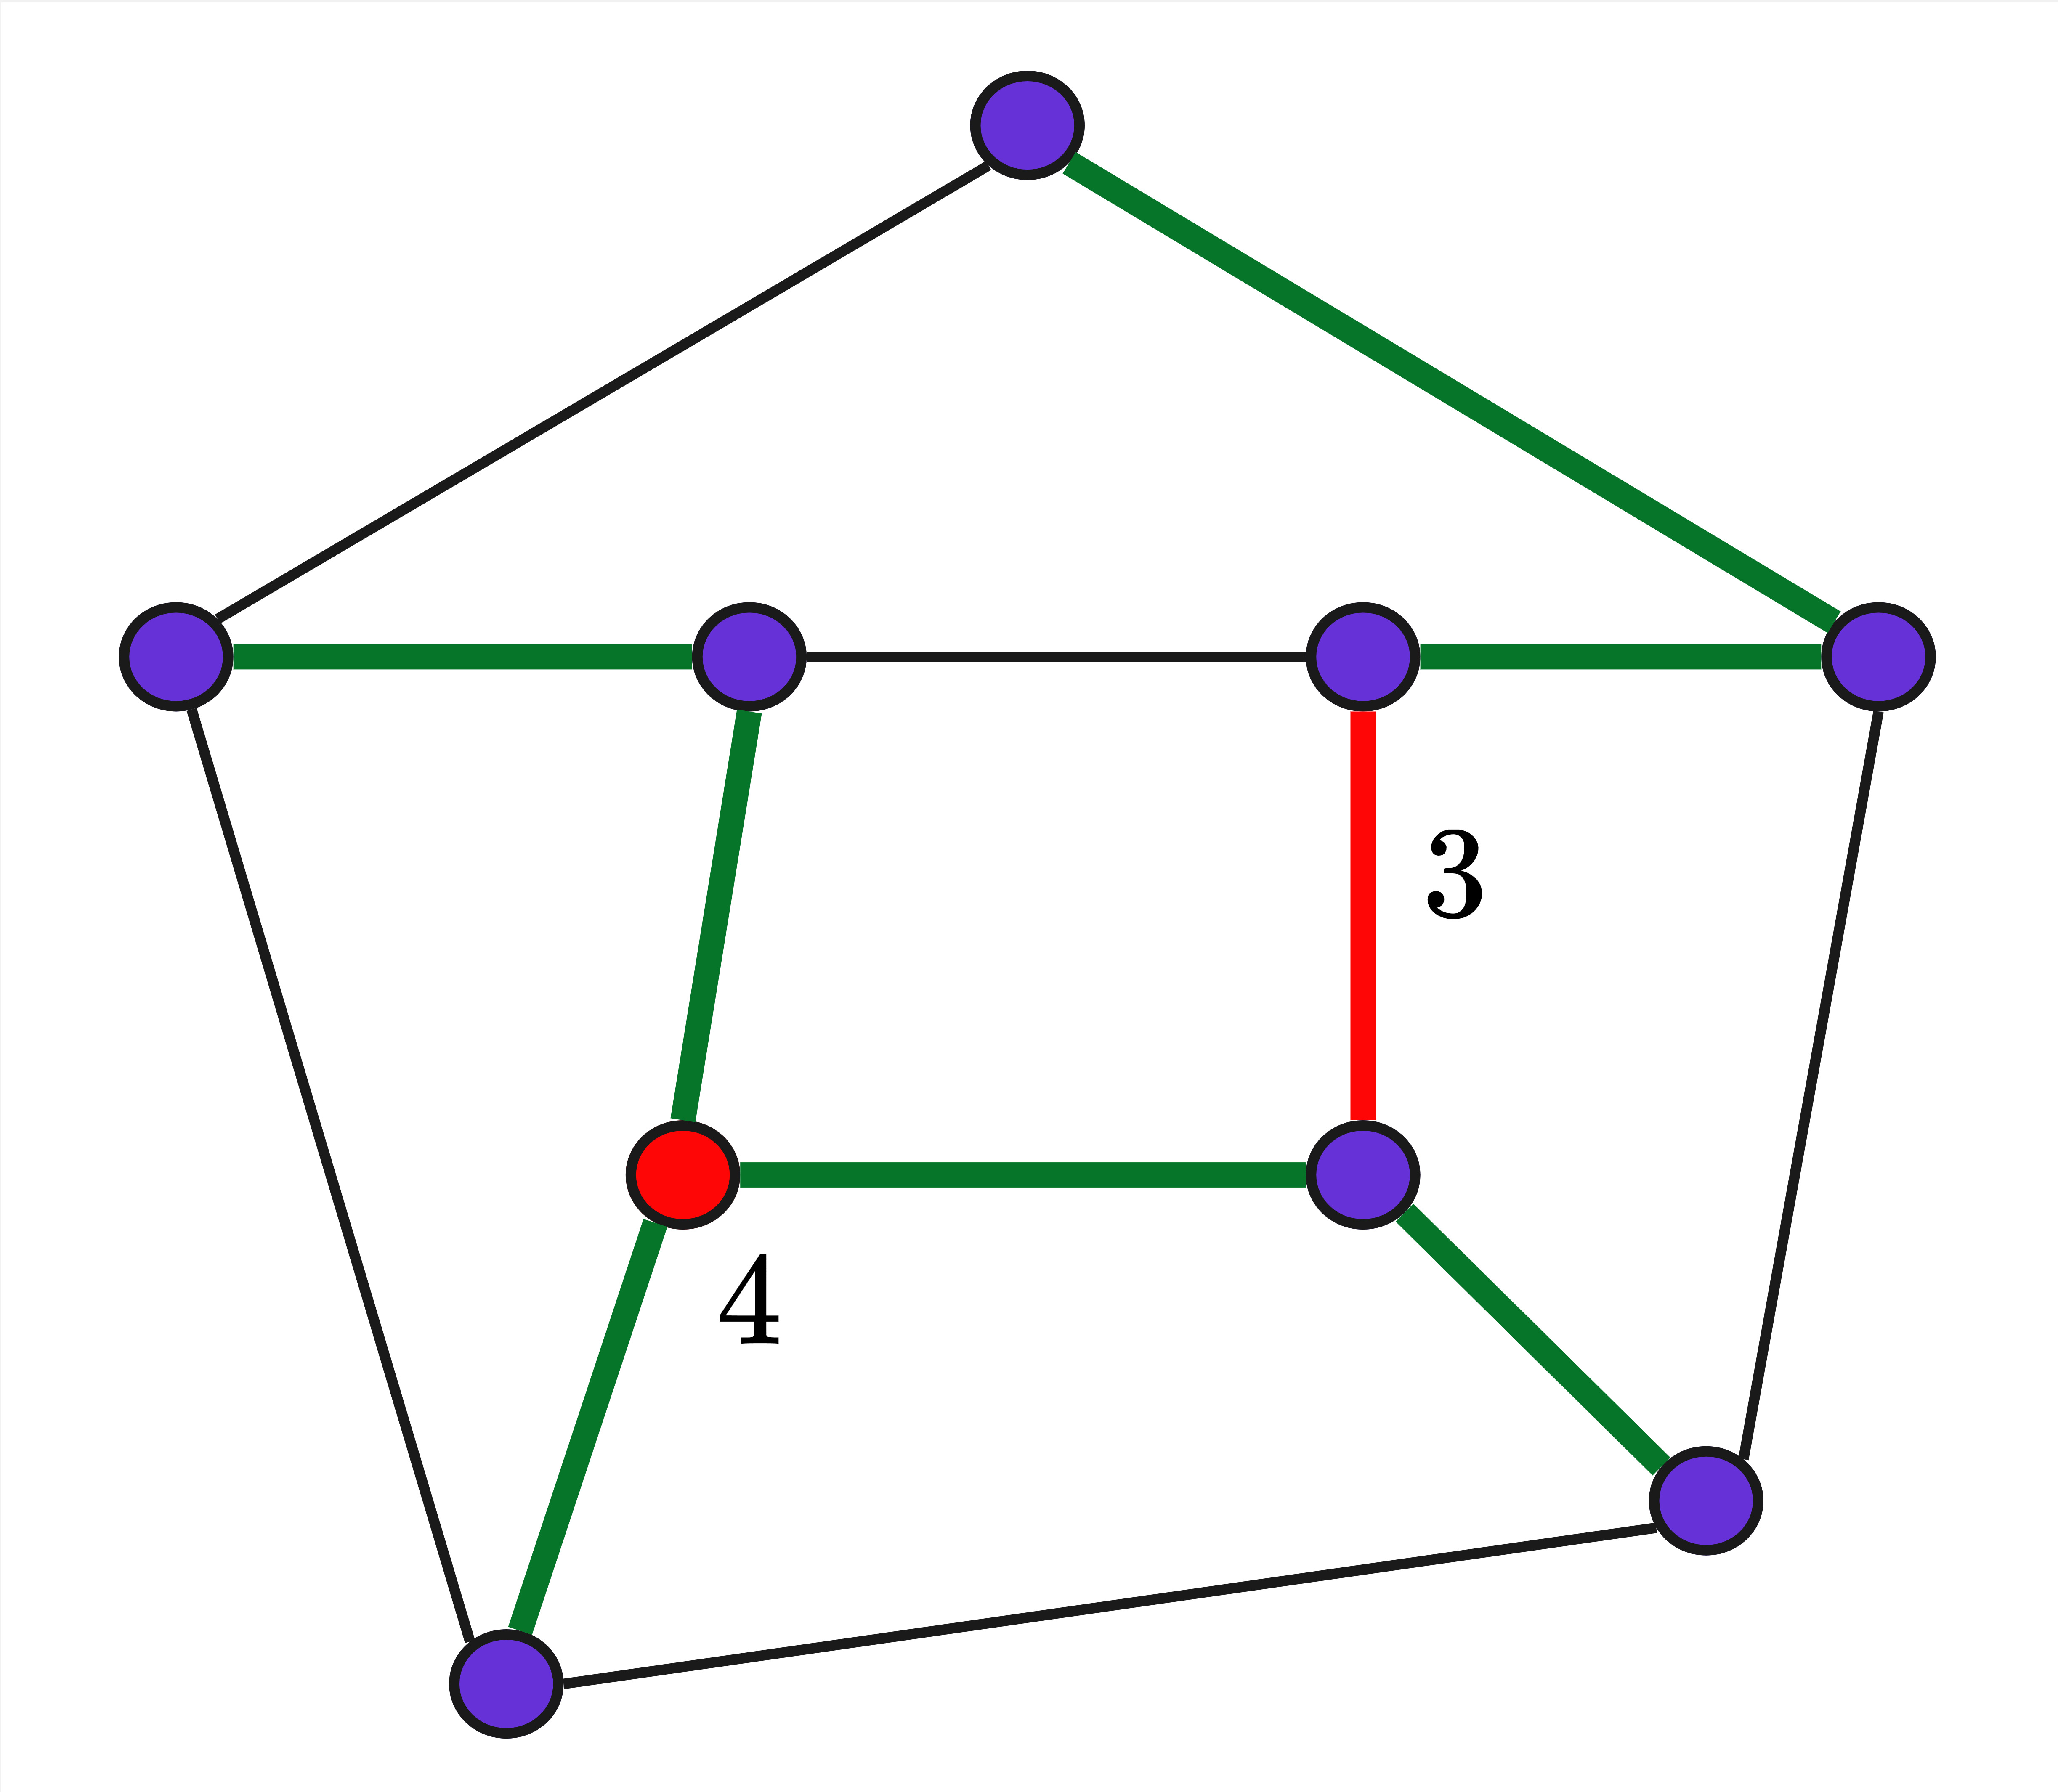
\includegraphics[width=7cm]{images/load_2.jpg}
    \end{minipage}
\end{frame}

\begin{frame}{Última Definição (desta seção)}
    \begin{defi}[Carga Máxima]
        A \emph{\textbf{carga máxima}} de uma floresta geradora maximal $(V, F)$ de um grafo $G$ é o maior valor entre as cargas de seus vértices $v \in V$ e arestas $e \in F$.
    \end{defi}
\end{frame}

\begin{frame}{Passo 2}
    \begin{lema}
        Todo grafo $k$-outerplanar com grau máximo 3 admite uma floresta geradora maximal com carga máxima $\leq 3k$.
    \end{lema}
    \bigbreak\pause
    Procedemos por indução em $k$.
\end{frame}

\begin{frame}{Passo 2\dots}
    \begin{proof}
    Suponha $k = 1$ e seja $R$ o conjunto de arestas da face externa da imersão de $G$:
    \begin{itemize}[-]
        \item Remova $R$; o grafo resultante é acíclico.
        \item Estenda $E \setminus R$ para uma floresta geradora maximal $F$, adicionando o máximo possível de arestas de $R$.
        \item Considere as arestas em $E \setminus F$ e as faces internas que elas formam.
        \item Cada aresta de $G$ delimita no máximo 2 faces internas, e cada vértice $v \in V$ participa de no máximo $\deg(v)$ delas.
    \end{itemize}
    \end{proof}
\end{frame}

\begin{frame}{Exemplo}
    \begin{minipage}{\linewidth}
        \centering
        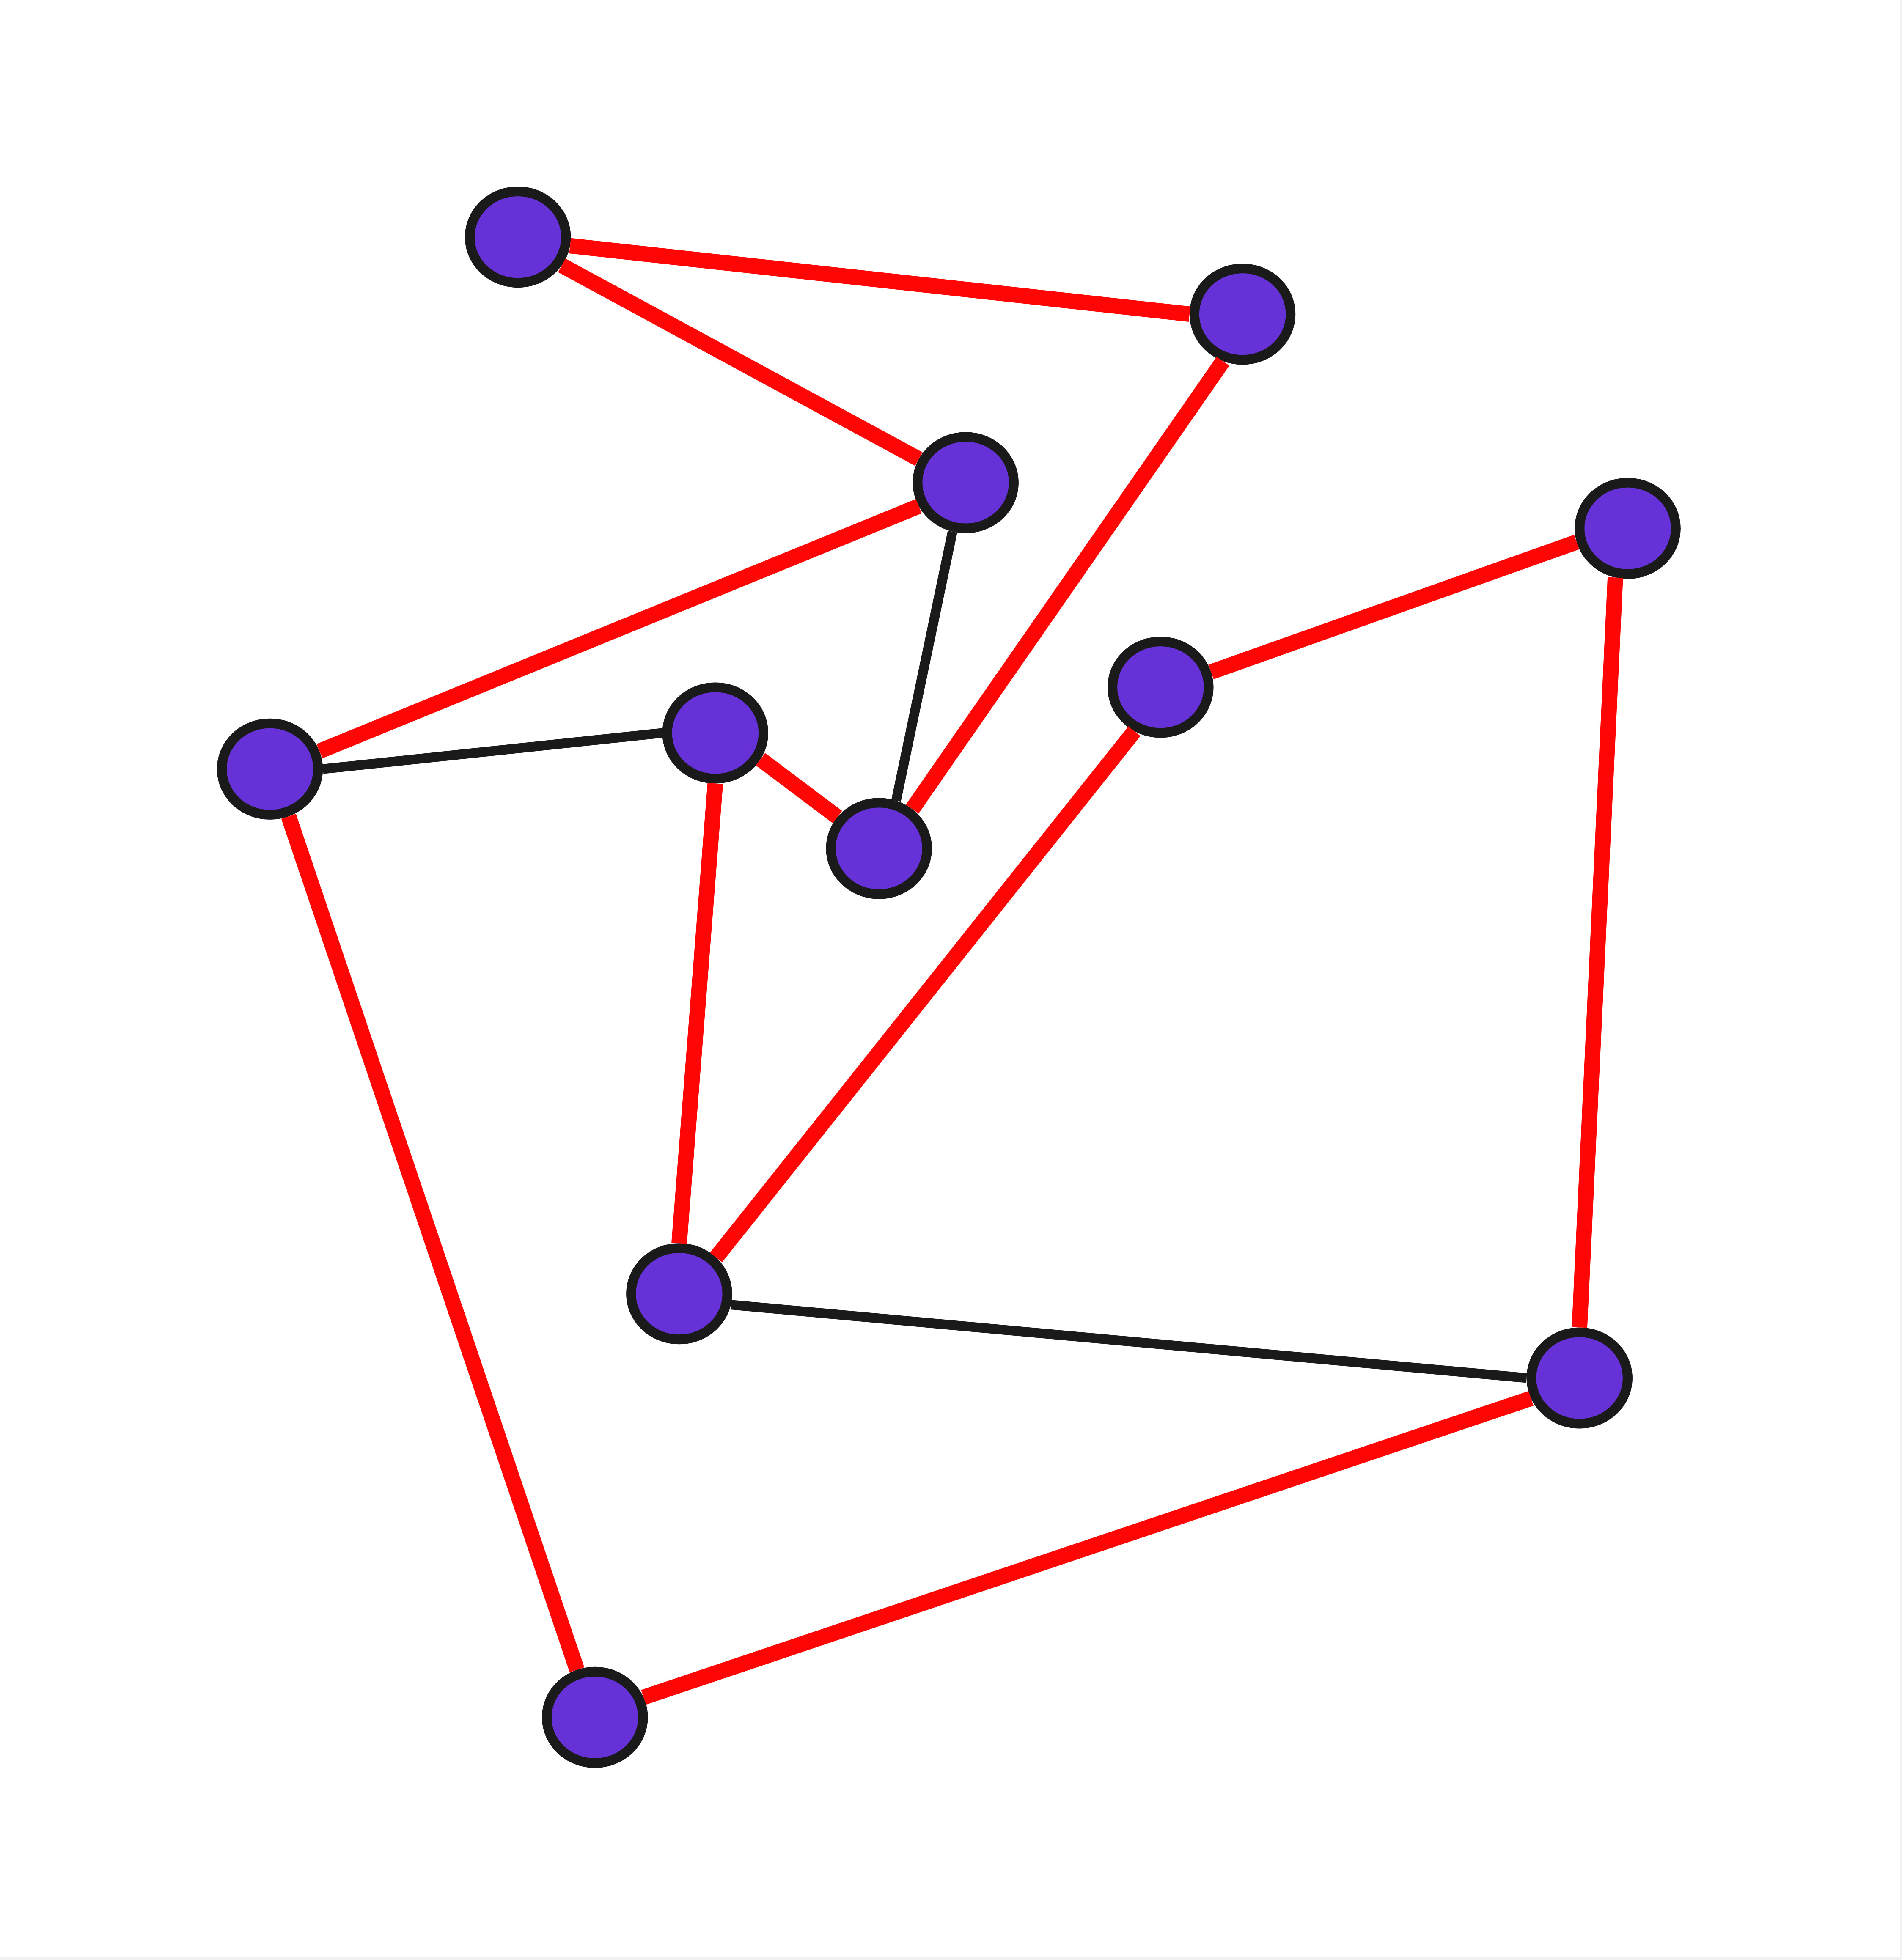
\includegraphics[width=8cm]{images/proof_2_1.jpg}
    \end{minipage}
\end{frame}

\begin{frame}{Exemplo}
    \begin{minipage}{\linewidth}
        \centering
        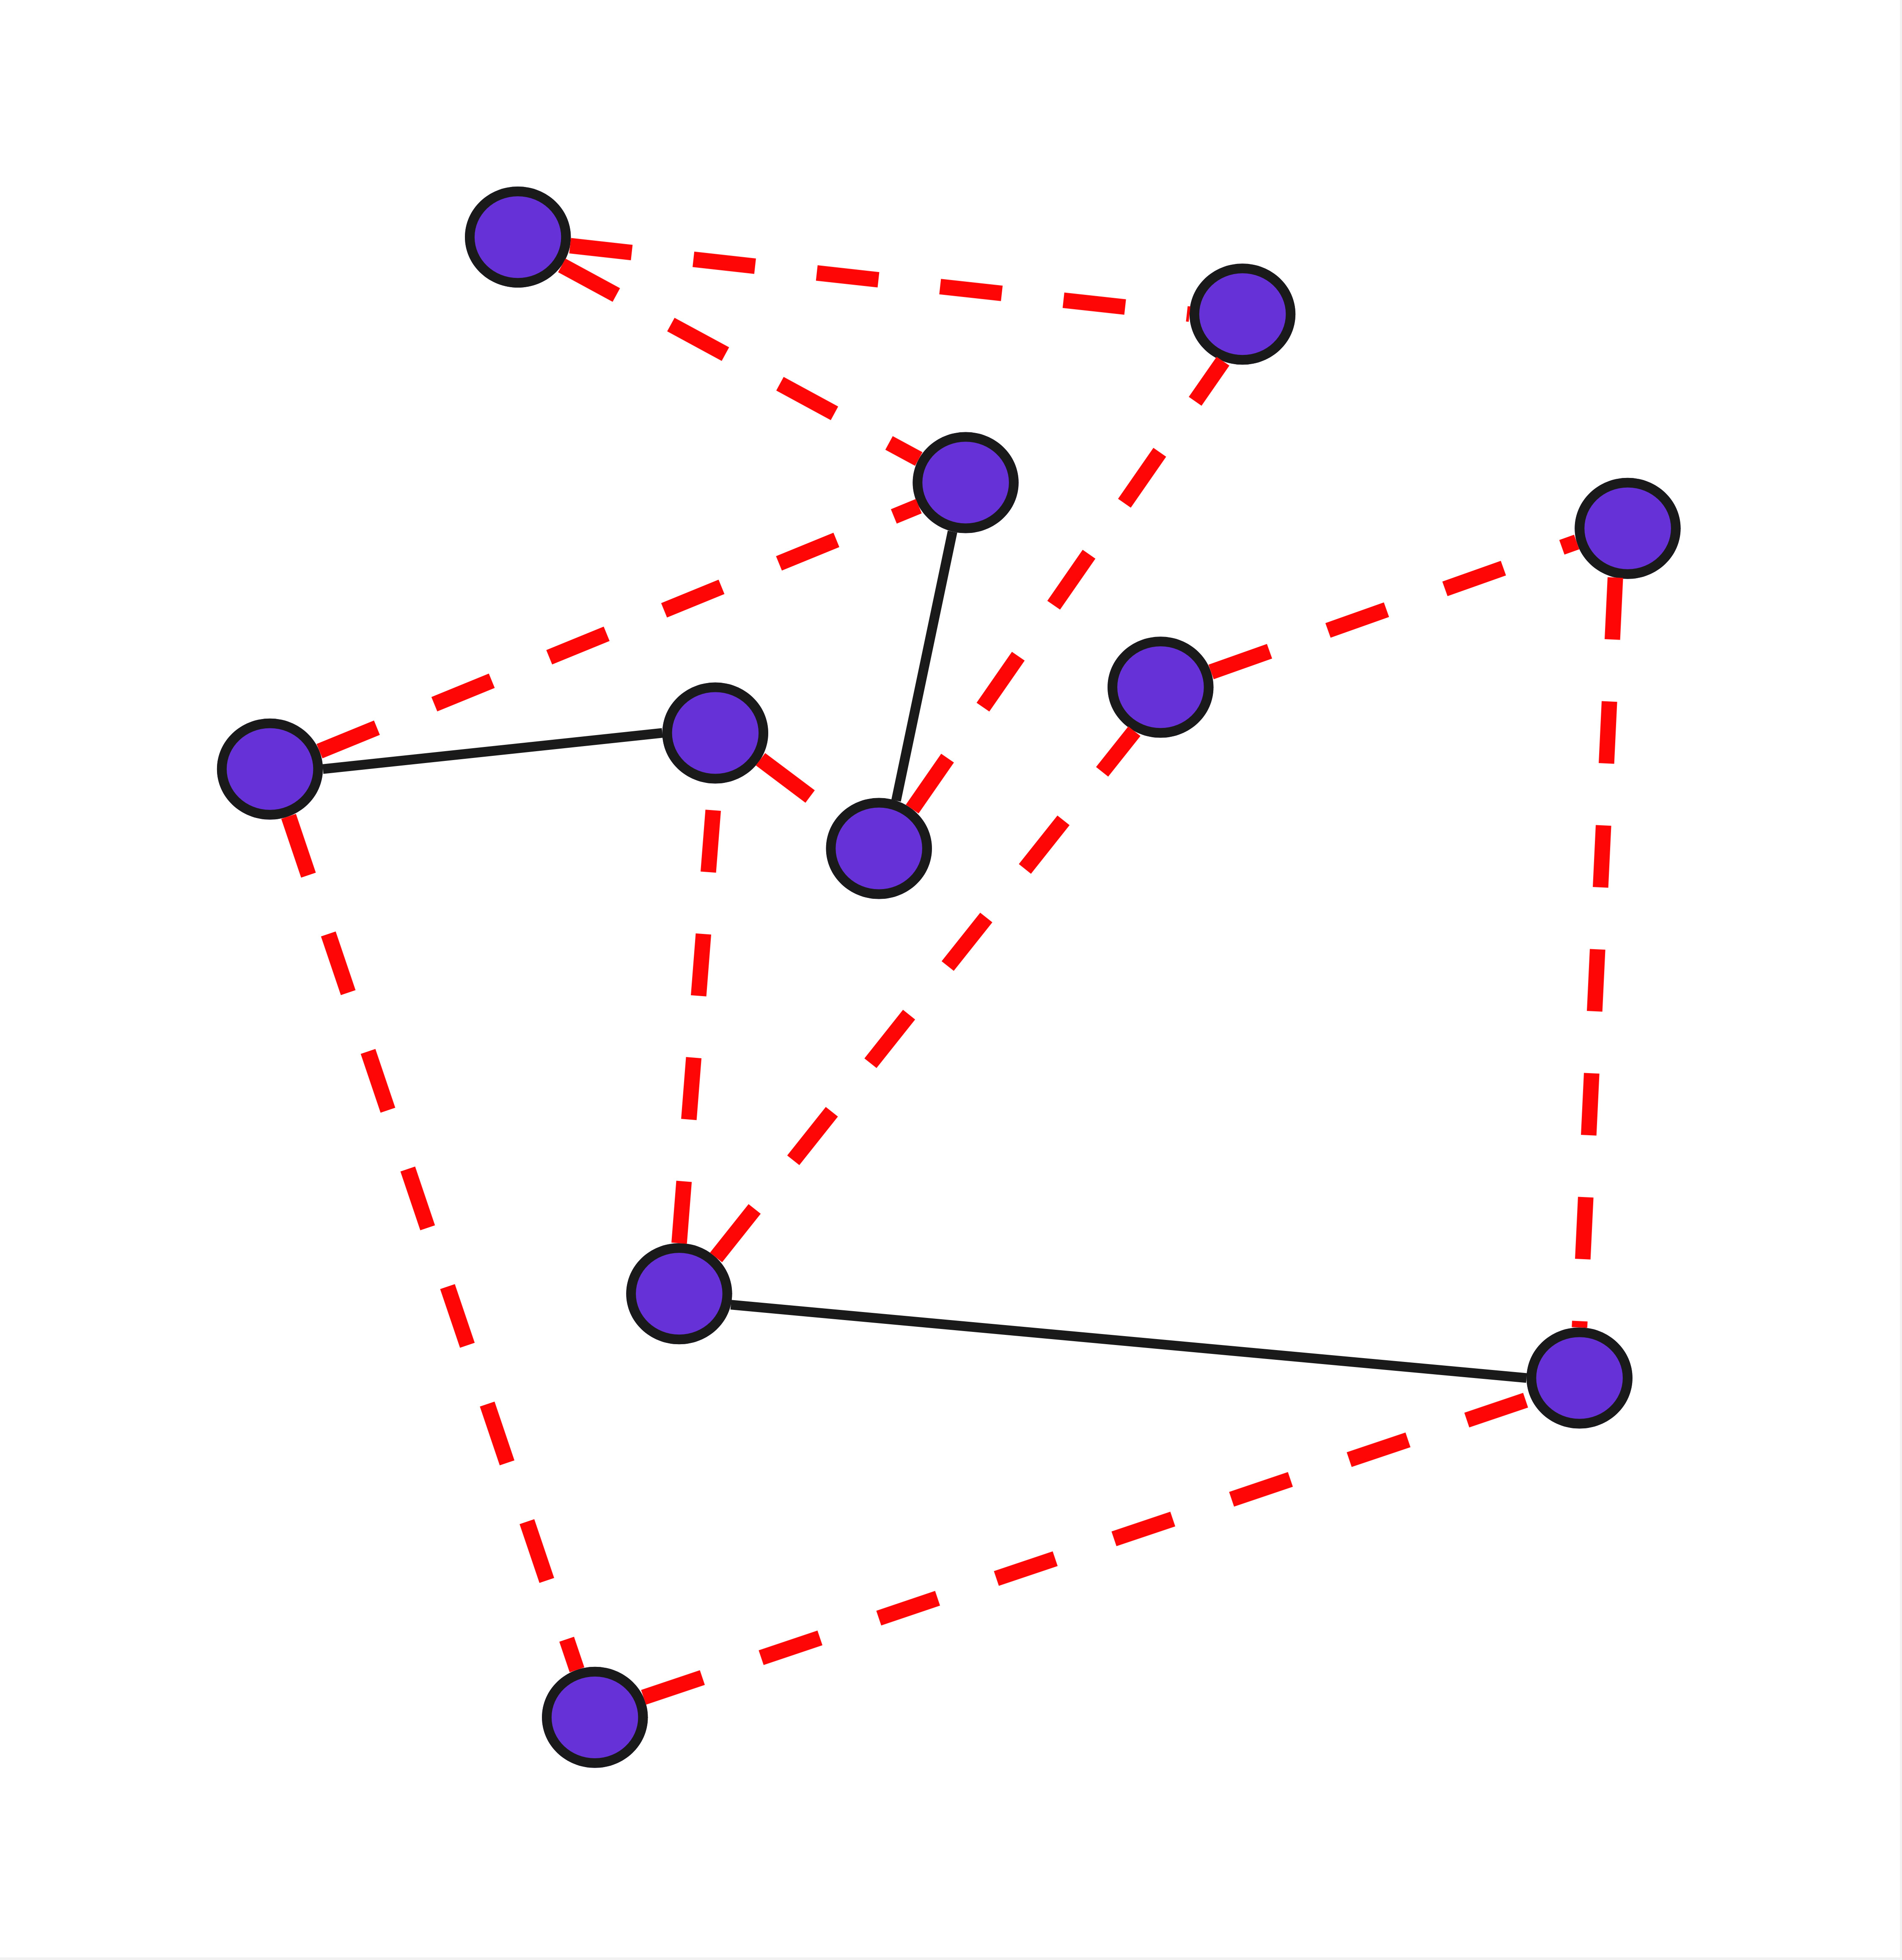
\includegraphics[width=8cm]{images/proof_2_2.jpg}
    \end{minipage}
\end{frame}

\begin{frame}{Exemplo}
    \begin{minipage}{\linewidth}
        \centering
        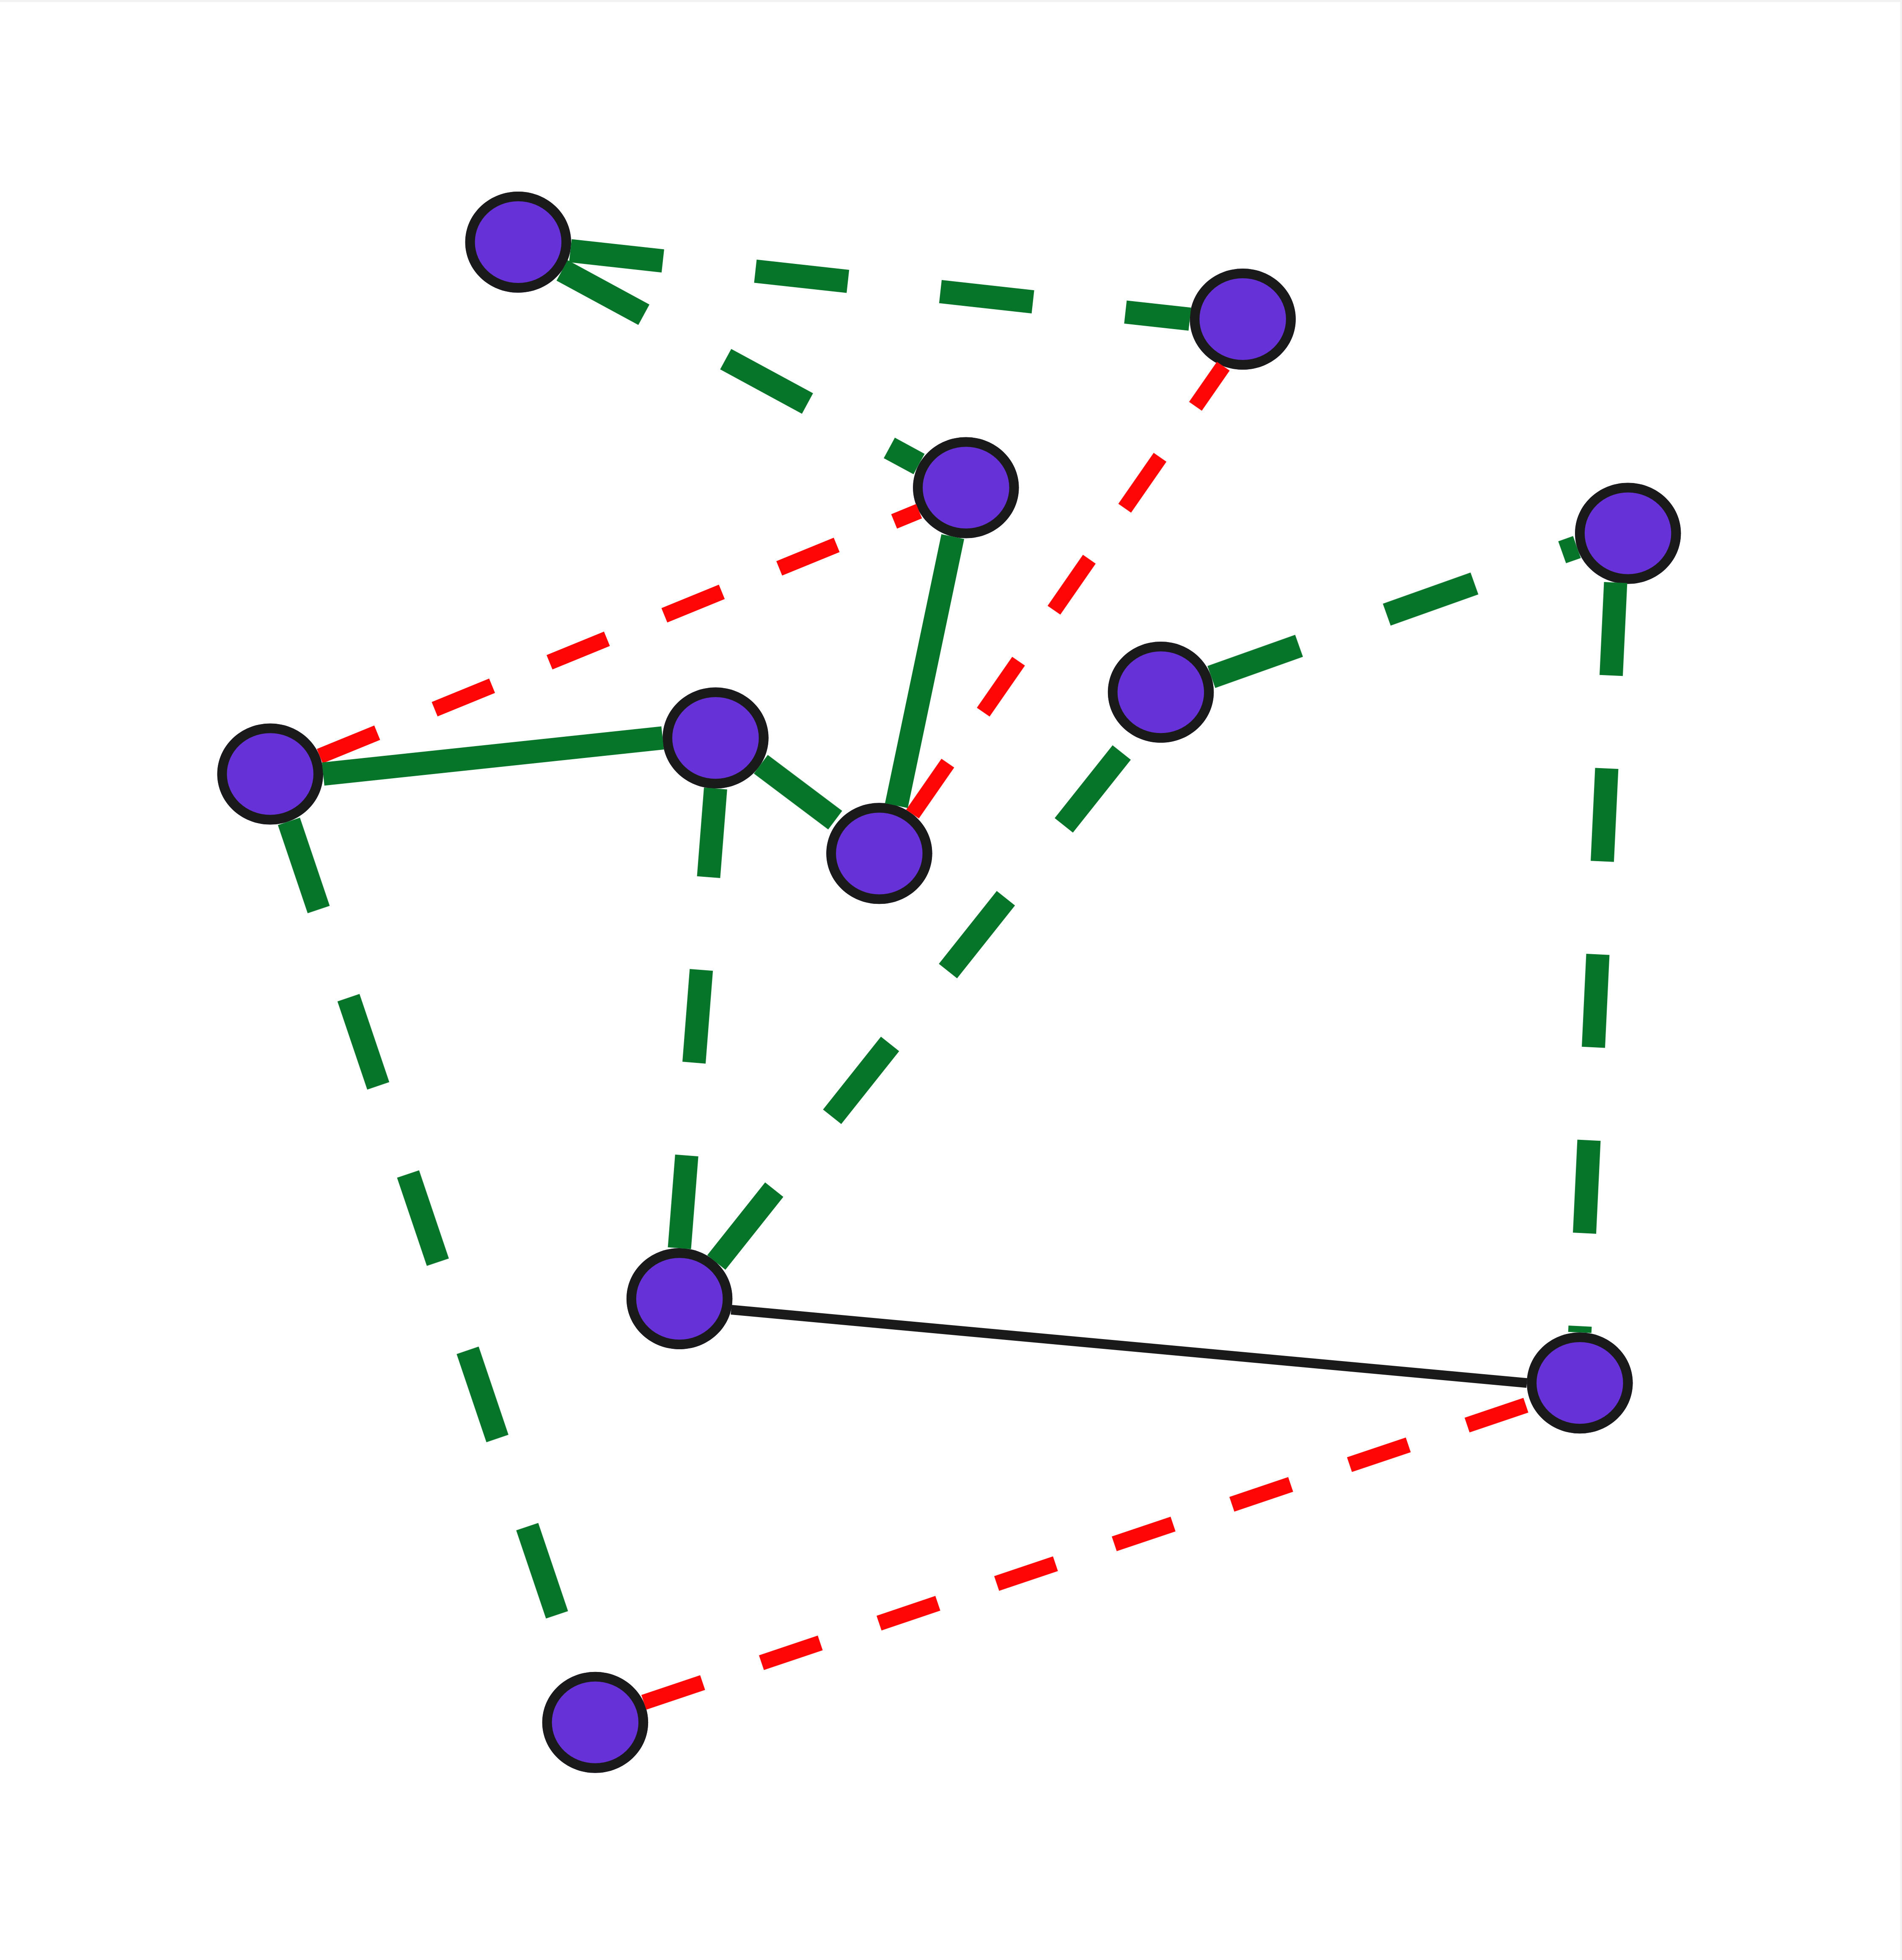
\includegraphics[width=8cm]{images/proof_2_3.jpg}
    \end{minipage}
\end{frame}

\begin{frame}{Passo 2\dots}
    \begin{proof}
        Para $k > 1$, seja $R$ o conjunto de arestas da face externa da imersão de $G$:
        \begin{itemize}[-]
            \item Remova $R$; o grafo restante é, no máximo, $(k - 1)$-outerplanar.
            \item Por indução, existe uma floresta geradora maximal $F^{\prime}$ com carga máxima $\leq 3(k - 1)$.
            \item Estenda $F^{\prime}$ para uma floresta geradora maximal $F$ de $G$, adicionando arestas de $R$.
            \item A carga adicional em qualquer aresta de $F$ é no máximo $2$, e em qualquer vértice, no máximo $3$.
        \end{itemize}
    \end{proof}
\end{frame}

\begin{frame}{Exemplo}
    \begin{minipage}{\linewidth}
        \centering
        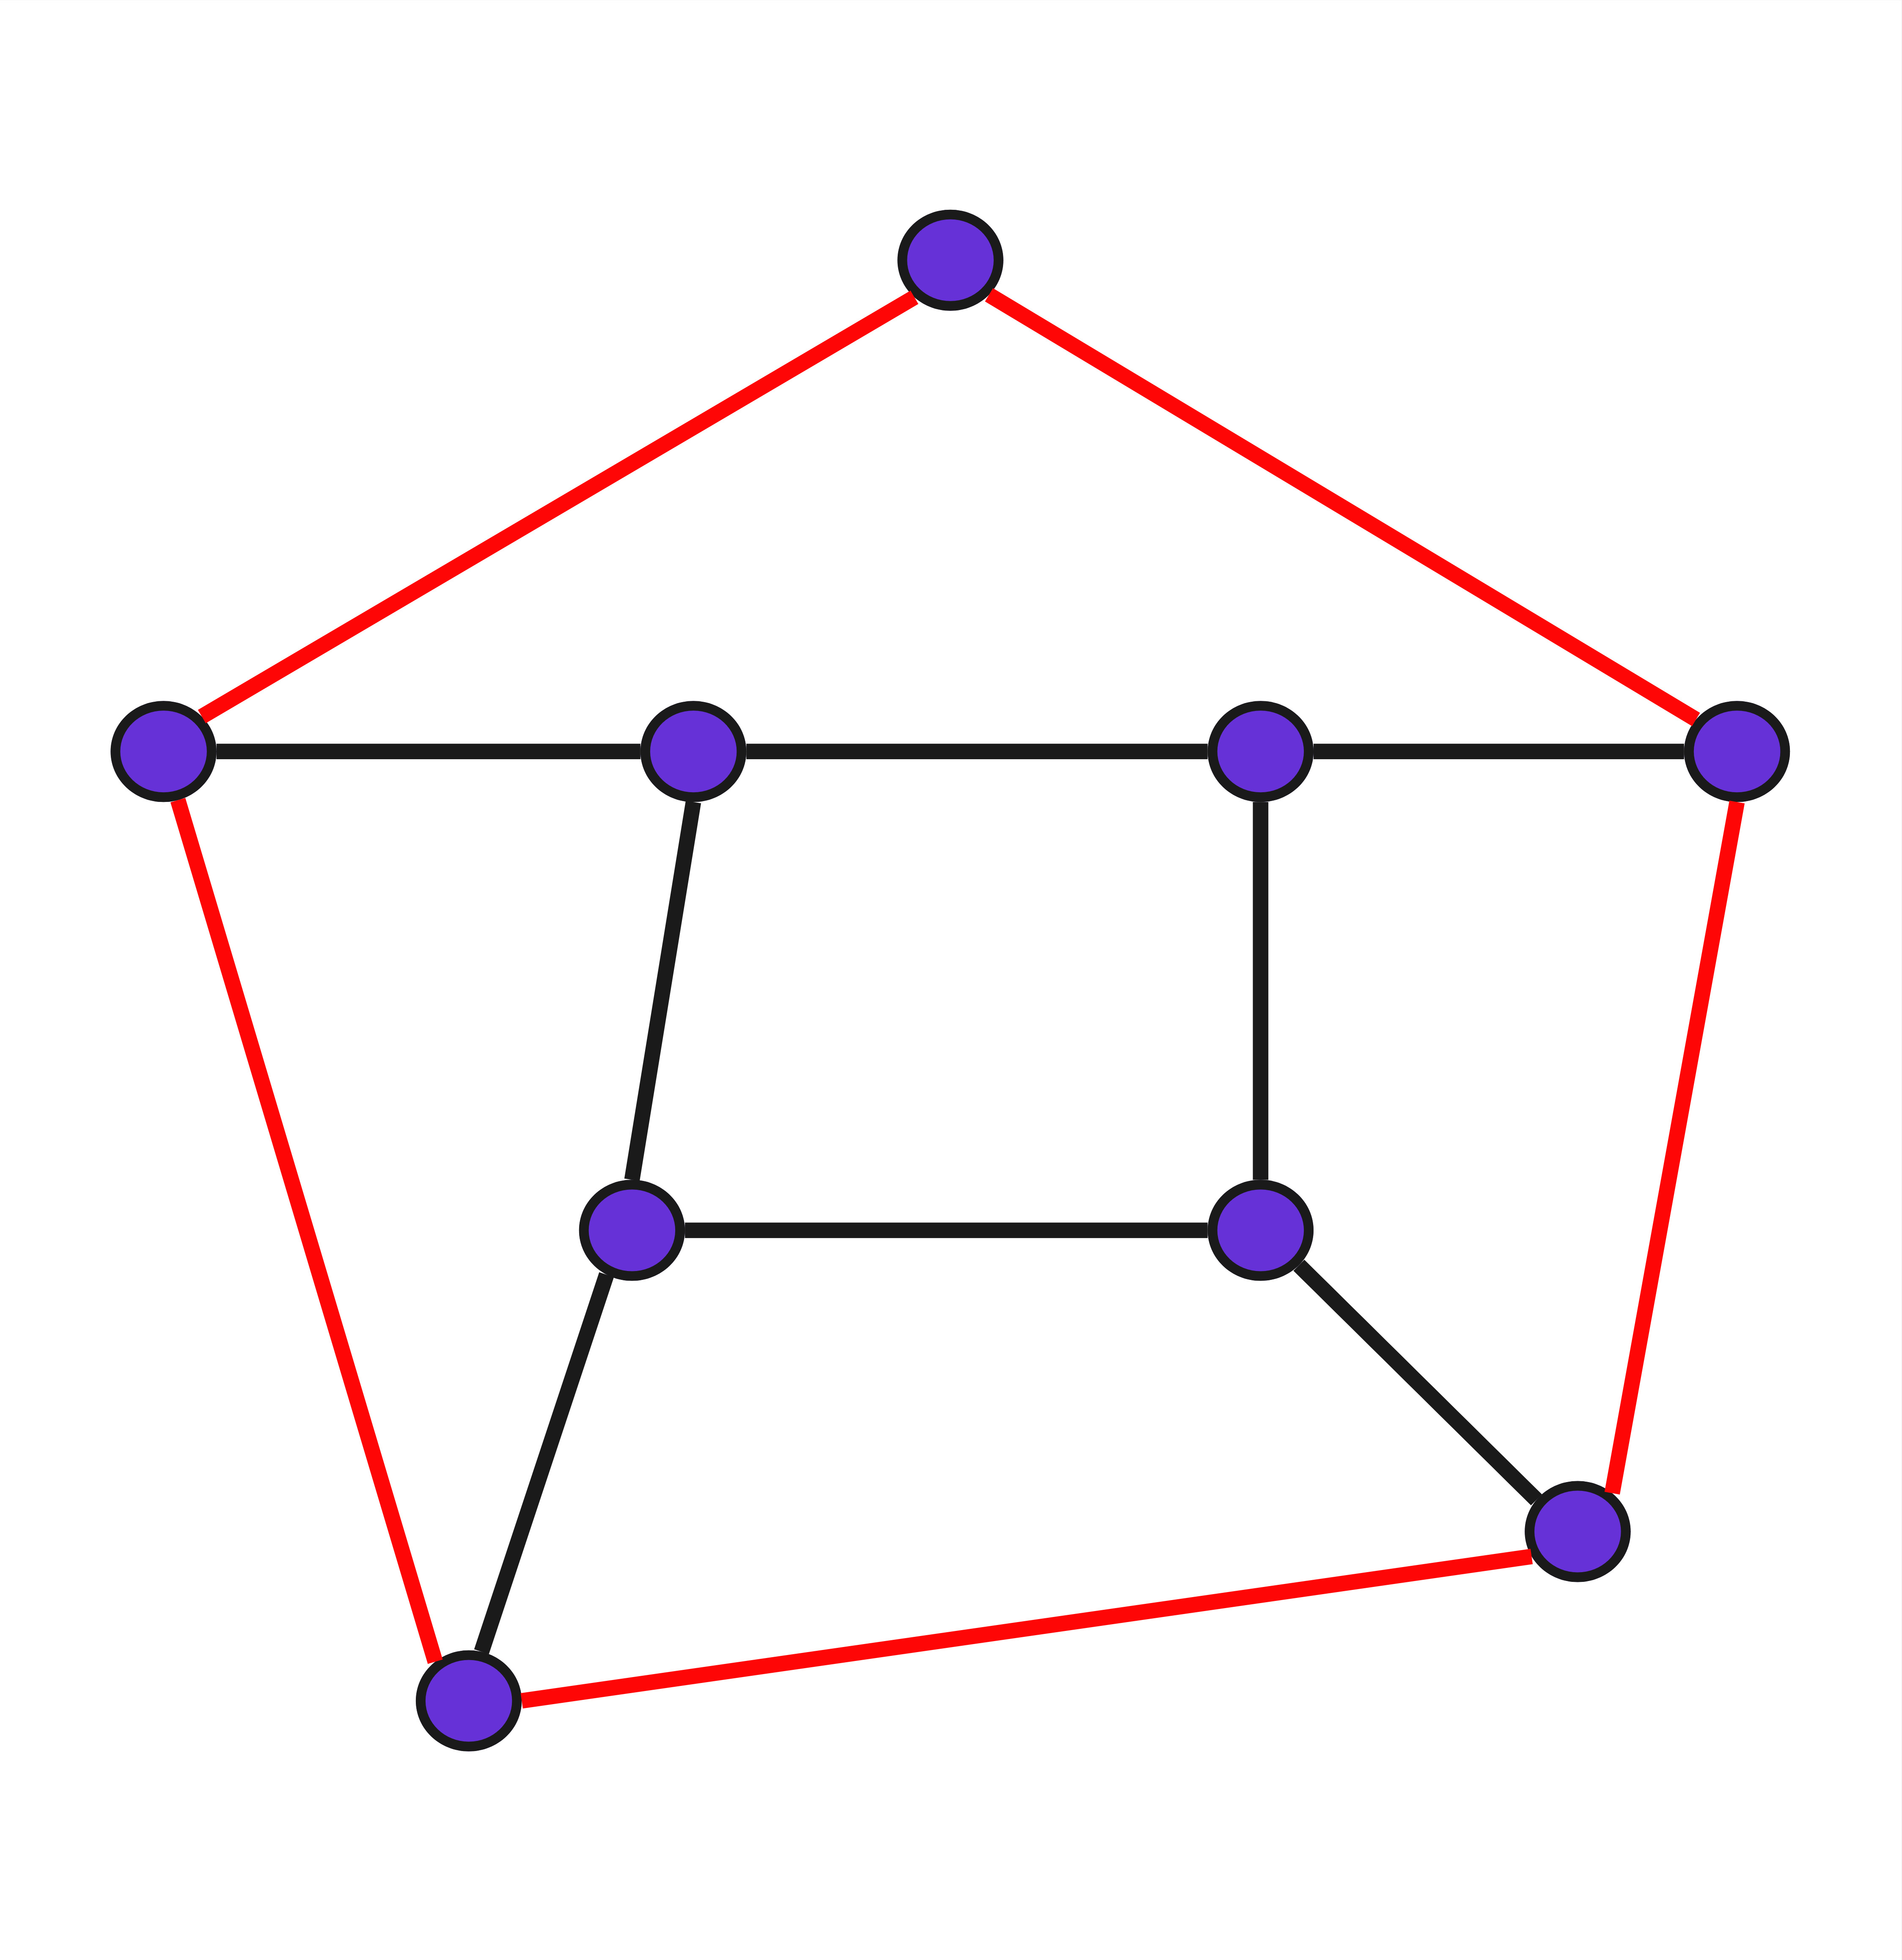
\includegraphics[width=8cm]{images/proof_2_4.jpg}
    \end{minipage}
\end{frame}

\begin{frame}{Exemplo}
    \begin{minipage}{\linewidth}
        \centering
        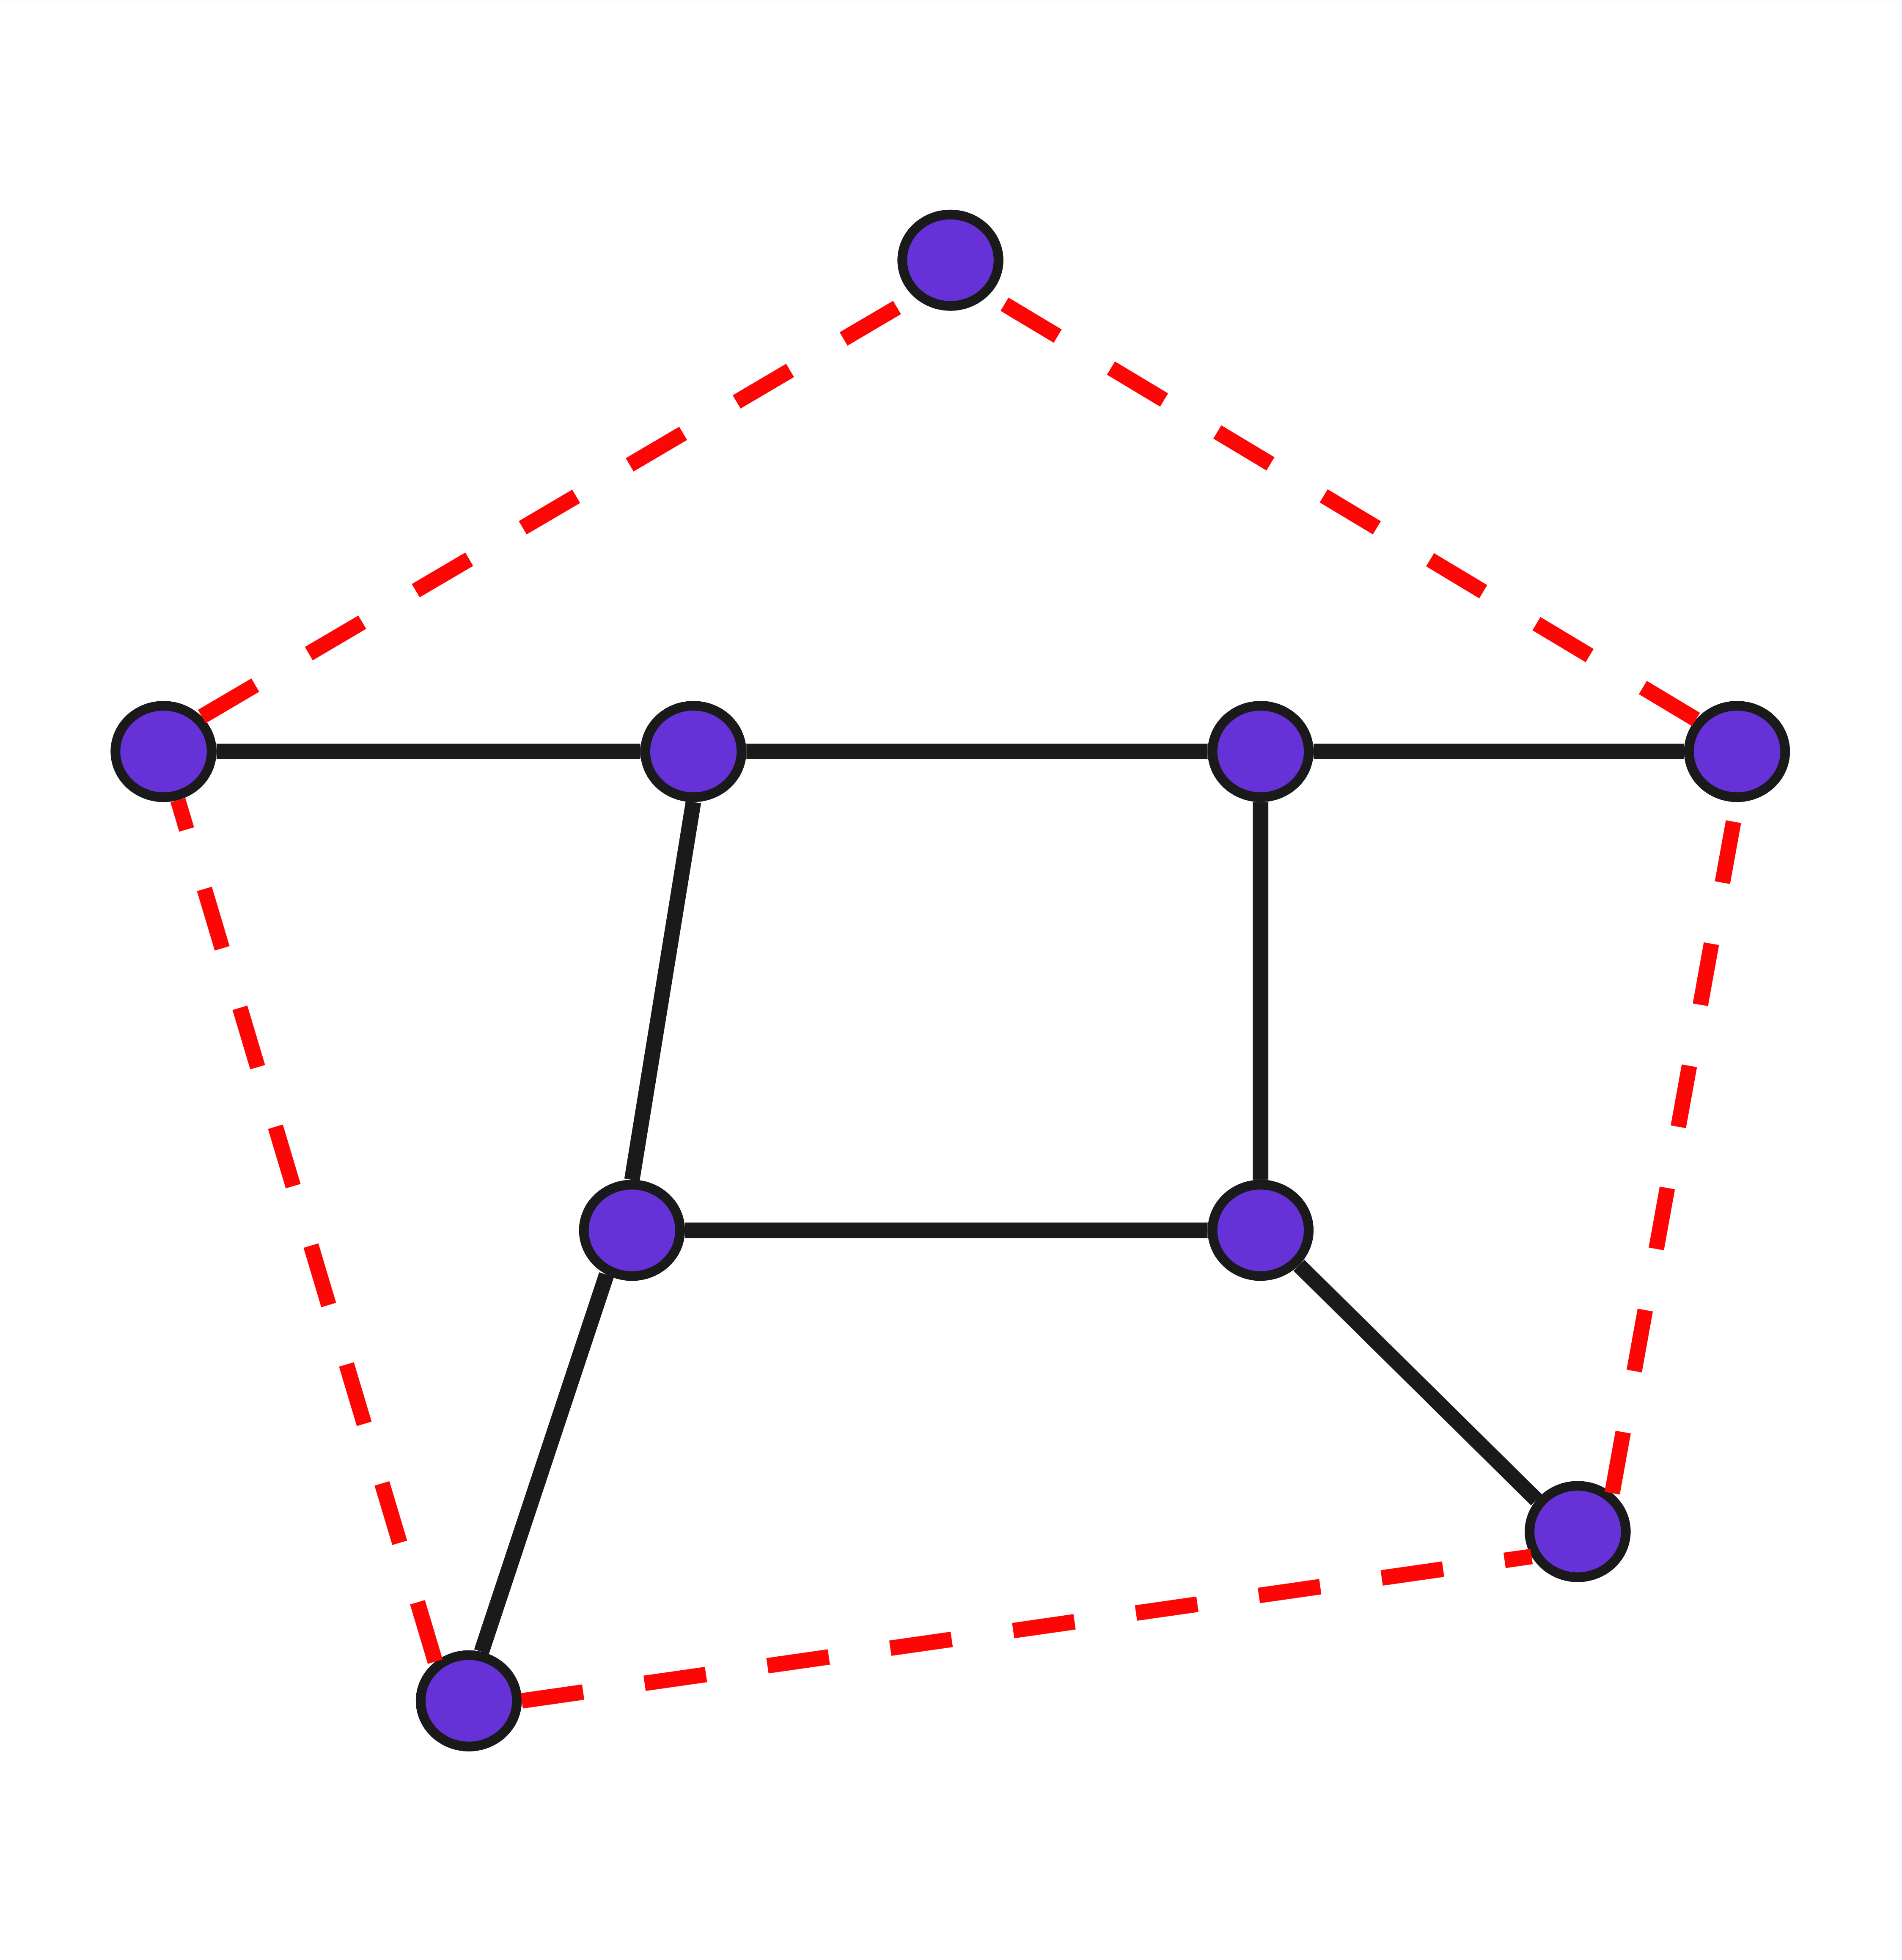
\includegraphics[width=8cm]{images/proof_2_5.jpg}
    \end{minipage}
\end{frame}

\begin{frame}{Exemplo}
    \begin{minipage}{\linewidth}
        \centering
        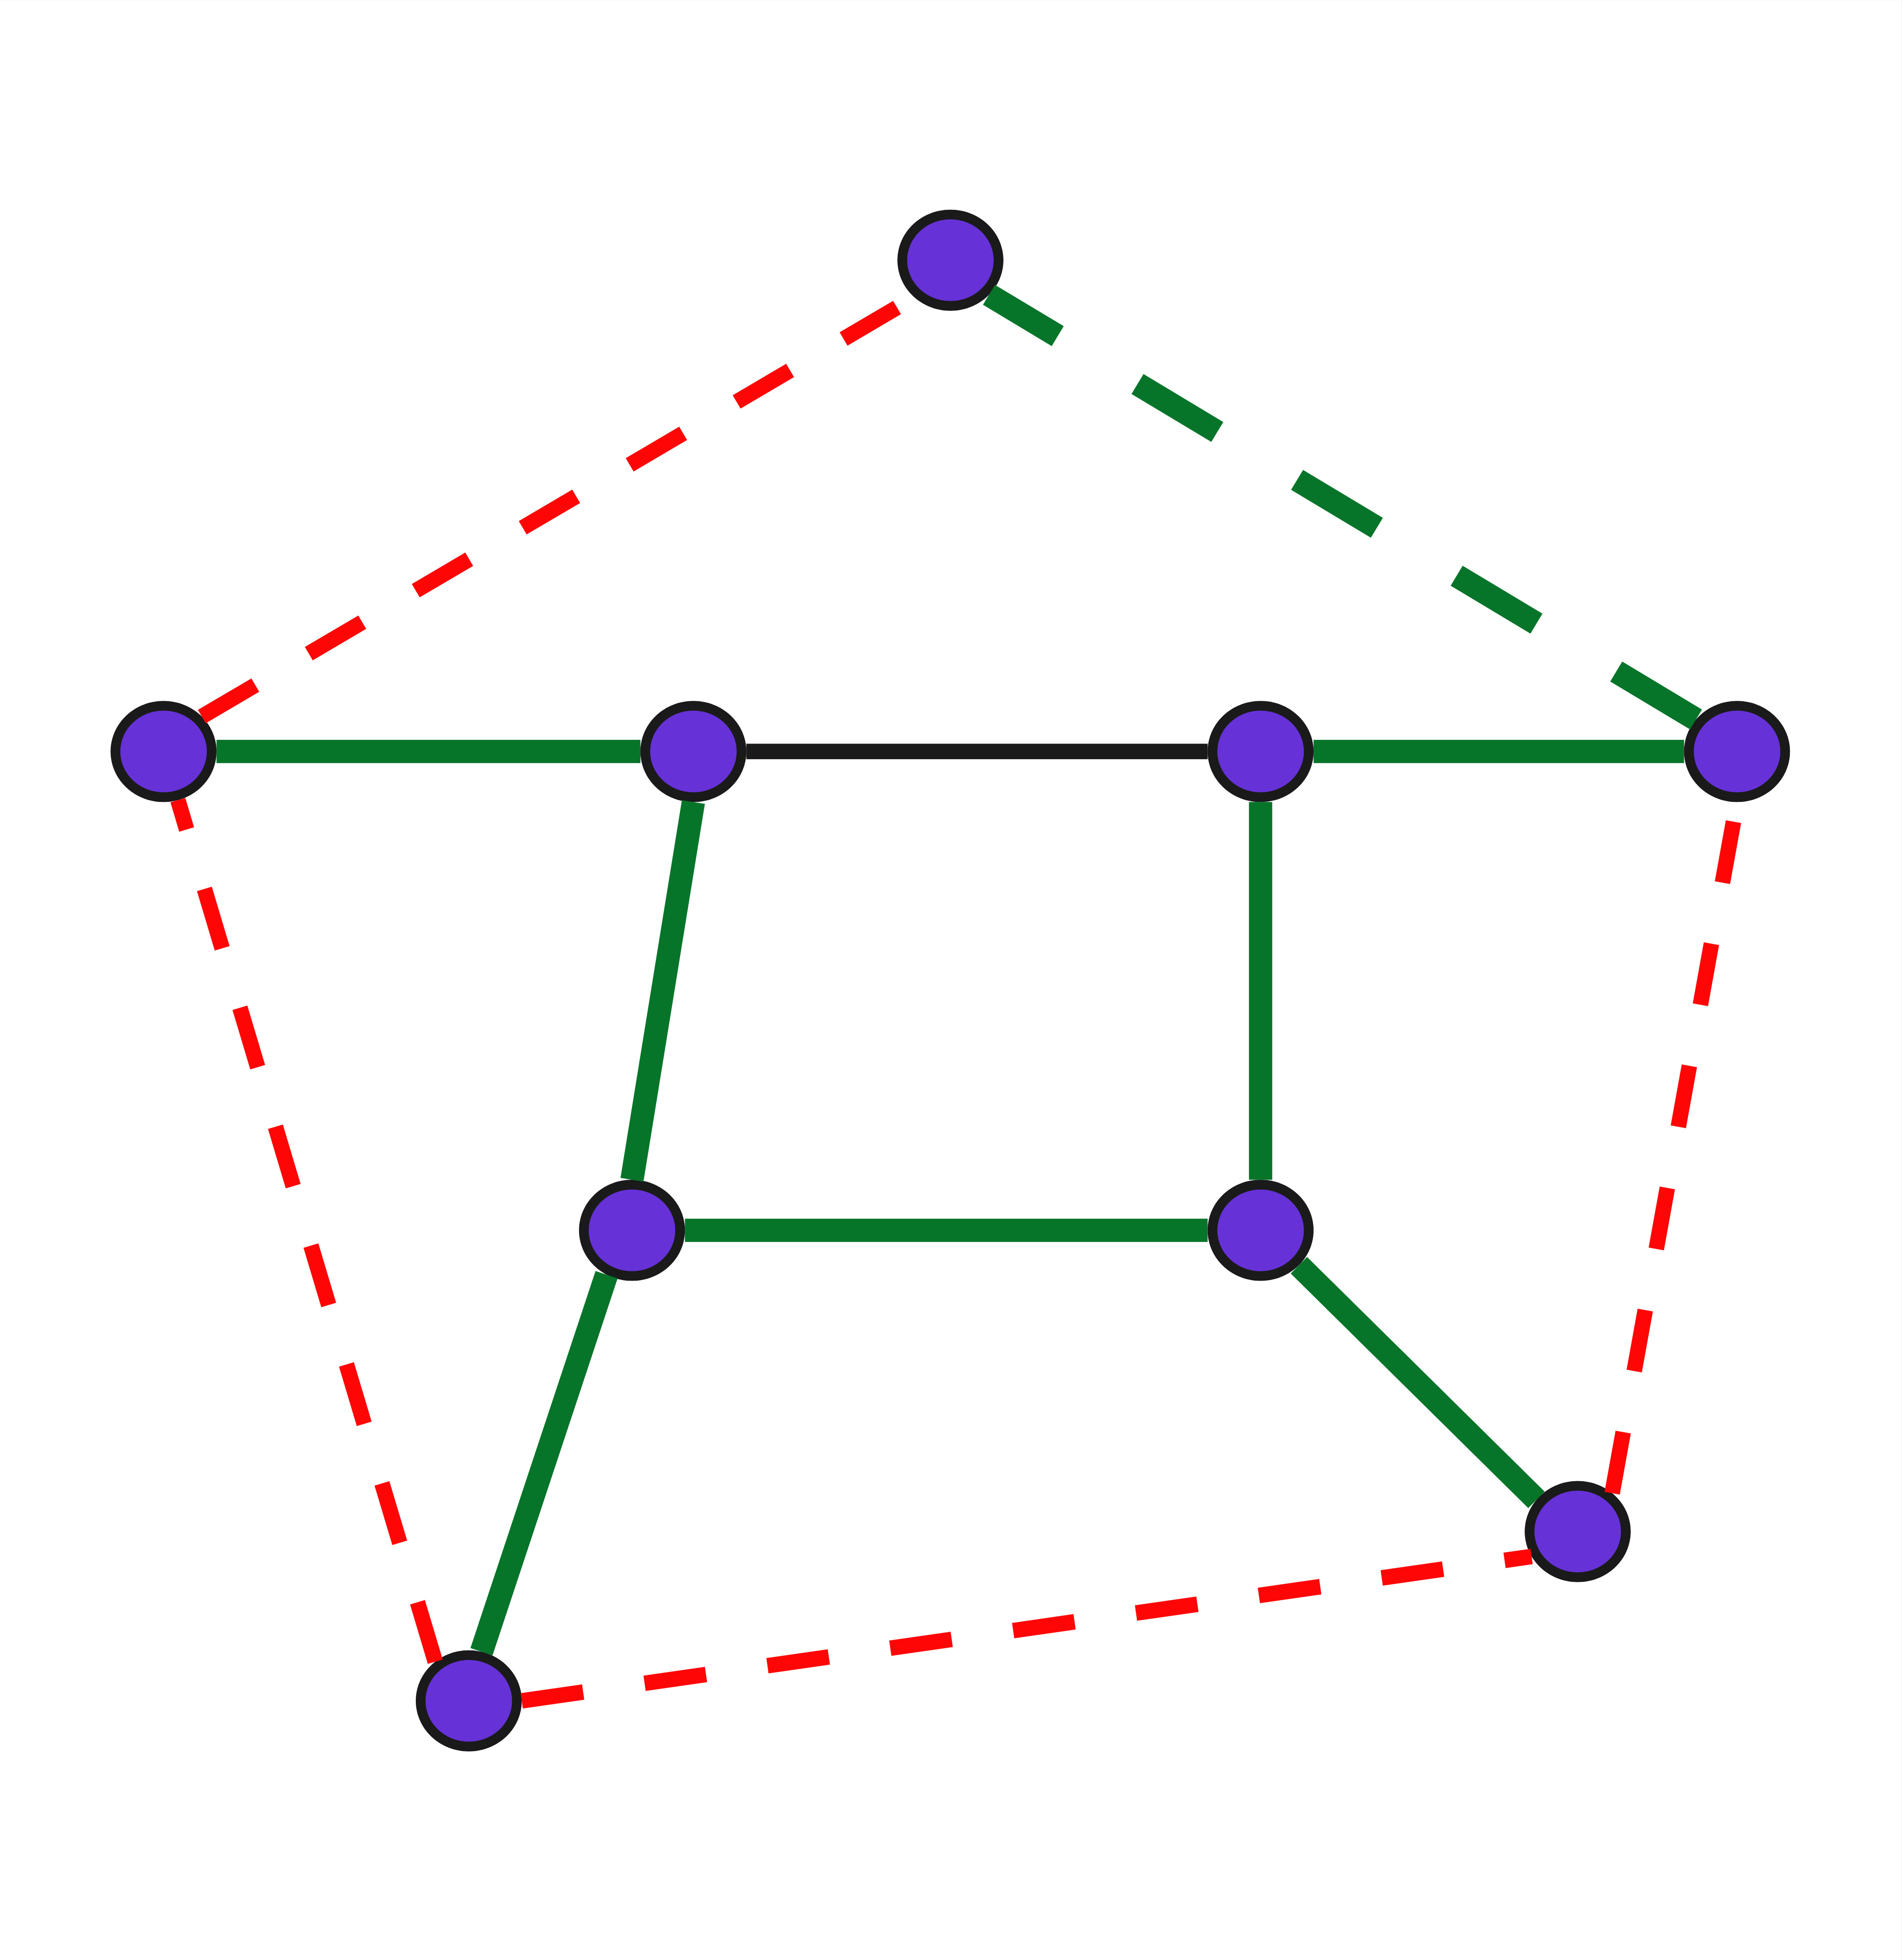
\includegraphics[width=8cm]{images/proof_2_6.jpg}
    \end{minipage}
\end{frame}

\begin{frame}{Passo 3}
    \begin{block}{Lema}
        Se um grafo $G$ de grau máximo 3 admite uma floresta geradora maximal $(V, F)$ com carga máxima $\leq \ell$, então a largura da árvore de $G$ é no máximo $\ell + 1$.
    \end{block}
\end{frame}

\begin{frame}{Passo 3\dots}
    \begin{proof}
        Construa uma decomposição em árvore para a floresta $F$ da seguinte forma:
        \begin{itemize}[-]
            \item Para cada vértice $u \in V$ e cada aresta $e = (v, w) \in F$, crie nós $t_u$ e $t_e$ em $T$.
            \item Iniciamos com $X_u = \{u\}$ e $X_e = \{v, w\}$.
            \item Para cada aresta $e = (u, v) \in E \setminus F$, escolha arbitrariamente um de seus extremos, digamos $u$.
            \item Para cada vértice $w \neq v$ no ciclo fundamental de $e$, adicione $u$ a $X_w$.
            \item Para cada aresta $e^\prime \in F$ no ciclo fundamental de $e$, adicione $u$ a $X_{e^\prime}$.
        \end{itemize}
        \phantom{\qedhere}
    \end{proof}
\end{frame}

\begin{frame}{Passo 3\dots}
    \begin{proof}
        Note que $(T, \{X_t\}_{t \in V(T)})$ é uma decomposição em árvore de $G$:
        \bigbreak

        \begin{itemize}
            \item \textbf{Propriedade 1:} Satisfeita trivialmente.
            \item \textbf{Propriedade 2:} Para $e = (u,v) \in E \setminus F$, $u$ foi adicionado a algum $X_{(w,v)}$ no ciclo fundamental de $e$, garantindo que $u$ e $v$ coexistem em um mesmo conjunto.
            \item \textbf{Propriedade 3:} Sempre que um vértice $v$ foi adicionado a subconjuntos, isso ocorreu ao longo de um caminho da árvore, mantendo a propriedade de conectividade.
        \end{itemize}
        \pause\bigbreak

        Cada conjunto $X_u$ ou $X_e$ recebeu no máximo tantos vértices quanto a carga de $u \in V$ ou $e \in F$, respectivamente. Como os conjuntos iniciais tinham no máximo 2 vértices, o tamanho final é no máximo $\ell + 2$.
        \alt<6>{\qedhere}{\phantom\qedhere}
    \end{proof}
\end{frame}

\begin{frame}{Exemplo}
    \begin{minipage}{\linewidth}
        \centering
        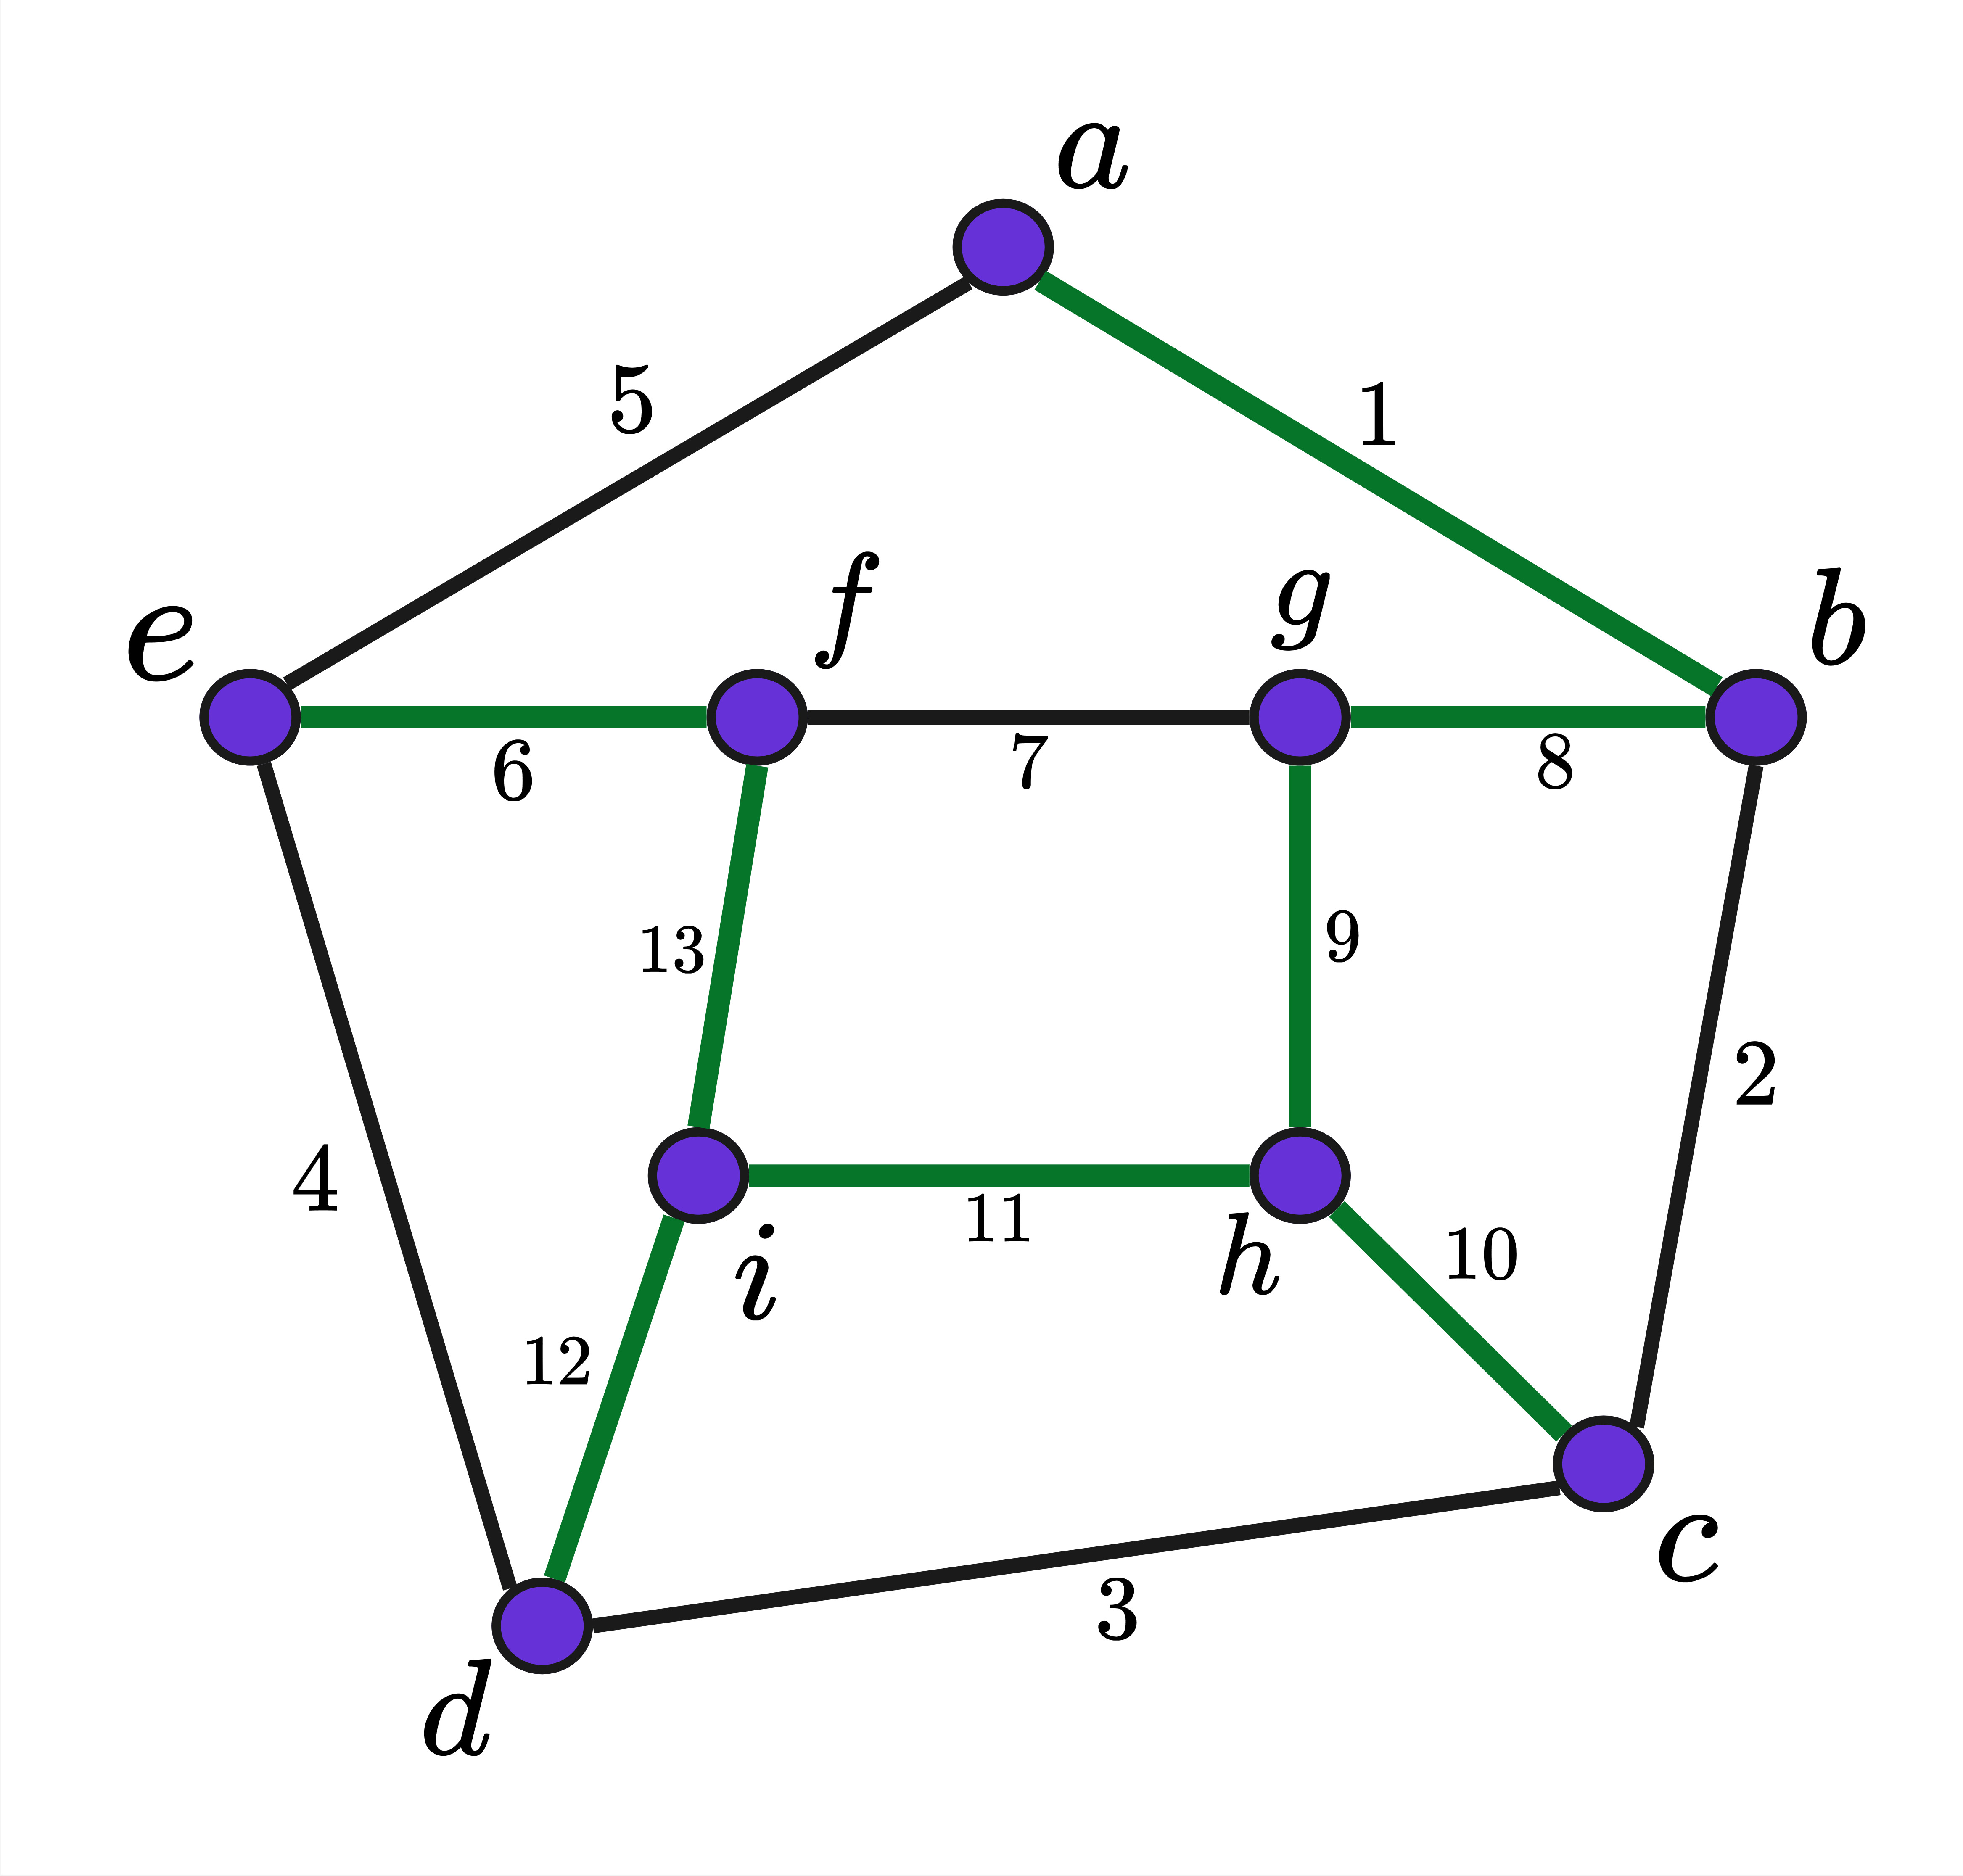
\includegraphics[width=8cm]{images/proof_3.jpg}
    \end{minipage}
\end{frame}

\begin{frame}{Lema Principal}
    \begin{lema}[1]
        \label{lema:1}
        Há um algoritmo para CI em grafos $k$-outerplanar que executa em tempo $2^{O(k)} \cdot n$.
    \end{lema}
\end{frame}


\section{Resultado Principal}
\begin{frame}{Teorema Principal}
    \begin{thm}[\cite{Cygan15, Will11}]
        \label{teo:2}
        Existe um algoritmo que, dada uma instância $I=(G, k)$ do problema CI em que $G$ é planar, resolve $I$ em tempo $2^{O(k)} \cdot n^{O(1)}$.
    \end{thm}
\end{frame}

\begin{frame}{Observação}
    \centering
    \vspace{1cm}
    \pause
    \Large Assim como ogros, grafos planares têm camadas!
    \begin{minipage}{\linewidth}
        \centering
        \vspace{1.73cm}
        
\includegraphics[height=5cm]{images/shrek.png}
    \end{minipage}
\end{frame}

\begin{frame}{Relembrando}
    \begin{minipage}{\linewidth}
        \centering
        \only<1>{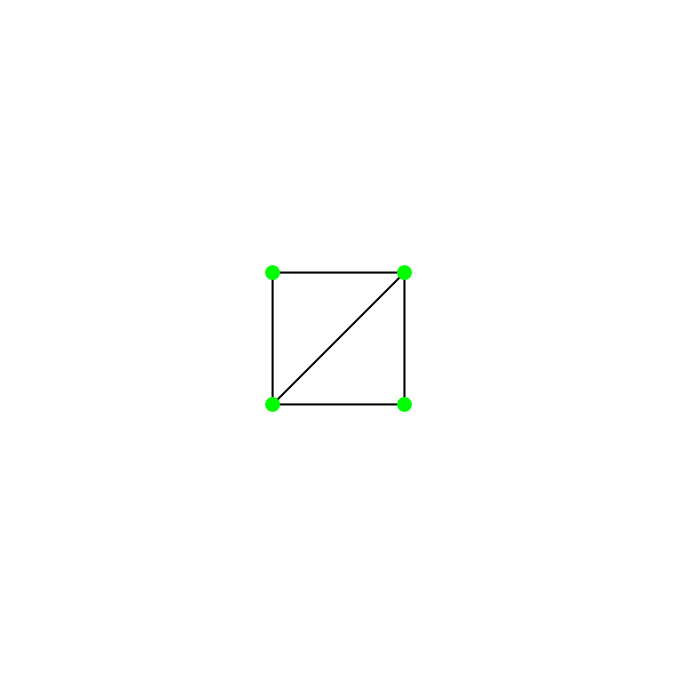
\includegraphics[height=6cm]{images/outer1.png}}
        \only<2>{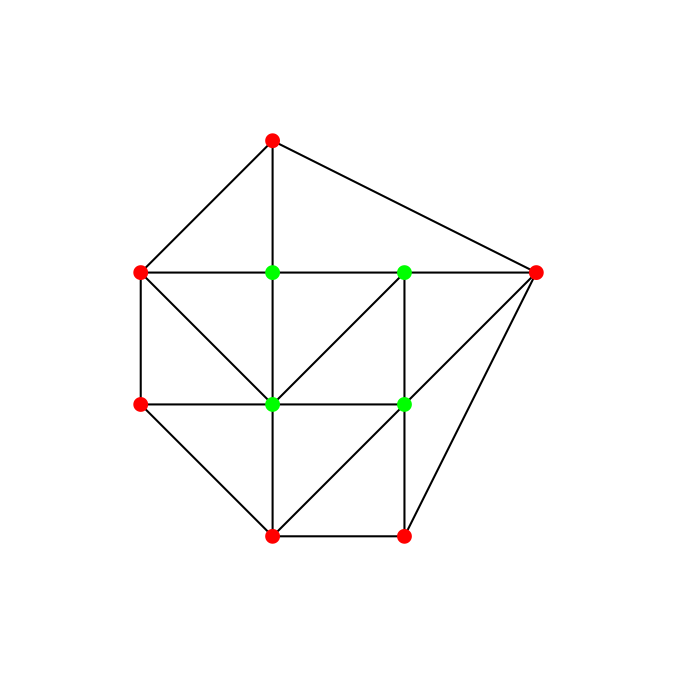
\includegraphics[height=6cm]{images/outer2.png}}
        \only<3>{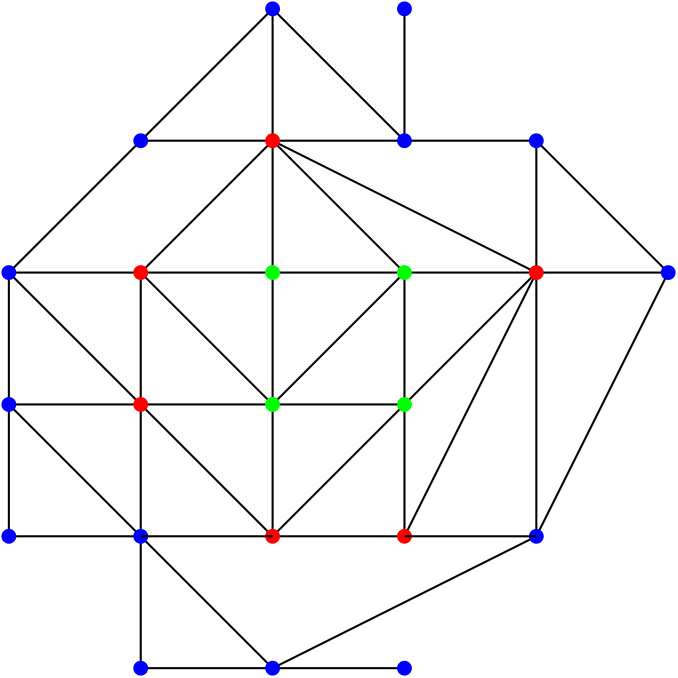
\includegraphics[height=6cm]{images/outer3.png}}
    \end{minipage}
\end{frame}

\begin{frame}{Preparação}
    Dado $G=(V, E)$ planar e $k \in \N^*$, definimos:
    \pause
    \begin{enumerate}[-]
        \item $\ell = k+1$;
        \item Para $0 \le i < \ell$, seja $S_i = \bigcup \{L_j \mid j \equiv i \pmod \ell\}$
        \begin{enumerate}[-]
            \item Ex.: $\ell = 4 \Rightarrow S_1 = L_1 \cup L_5 \cup L_9 \cup \dots$
        \end{enumerate}
        \item $G_i = G[V - S_i]$.
    \end{enumerate}
\end{frame}

\begin{frame}{Decomposição em \emoji{onion}}
    \centering
    \Large $\ell=3$:
    \bigbreak
    \begin{minipage}{\linewidth}
        \centering
        \only<1>{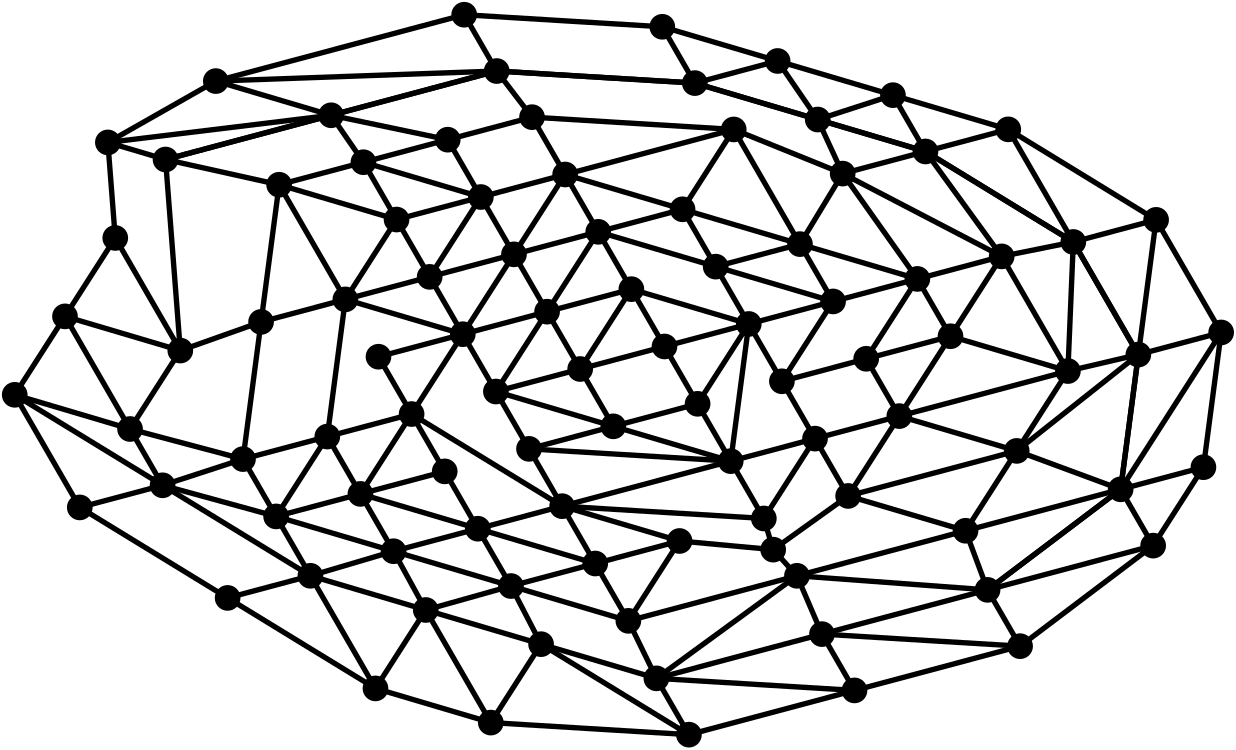
\includegraphics[height=4cm]{images/onion1.png}}
        \only<2>{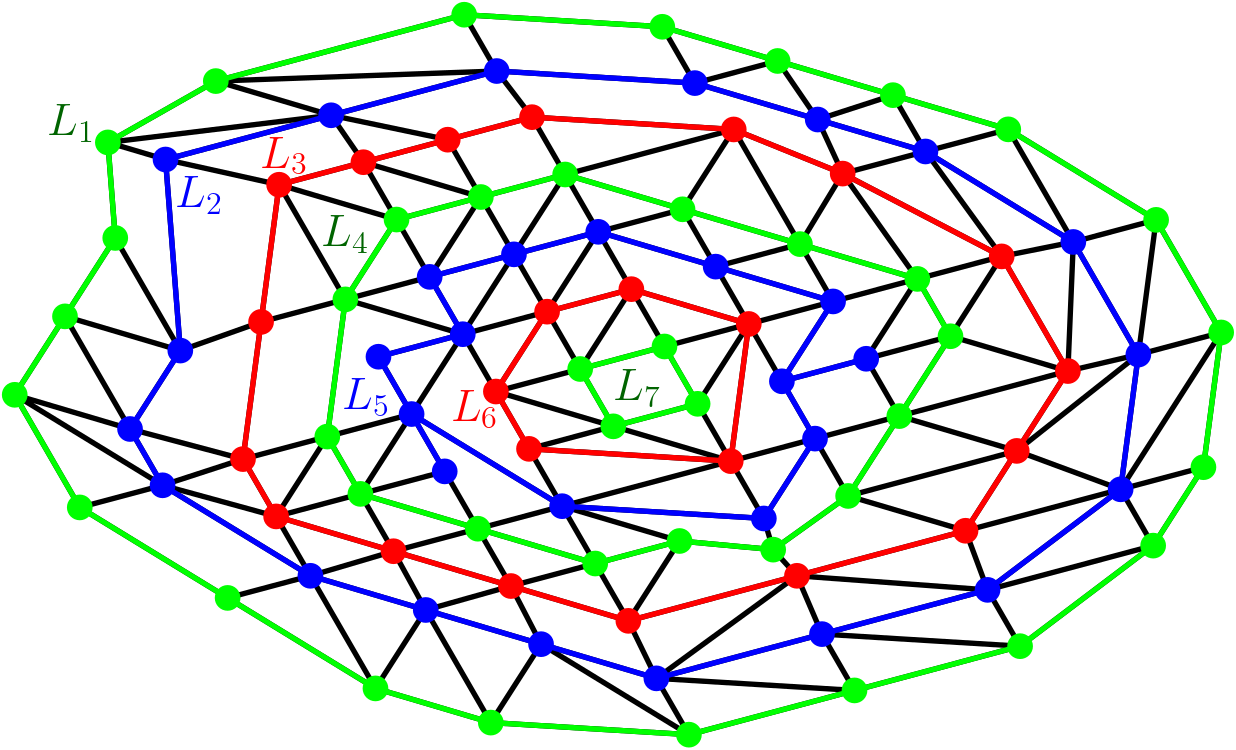
\includegraphics[height=4cm]{images/onion2.png}}
        \only<3>{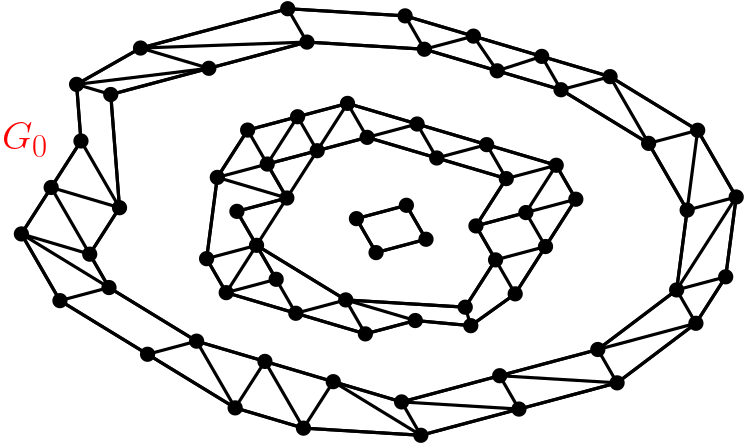
\includegraphics[height=4cm]{images/onion3.png}}
        \only<4>{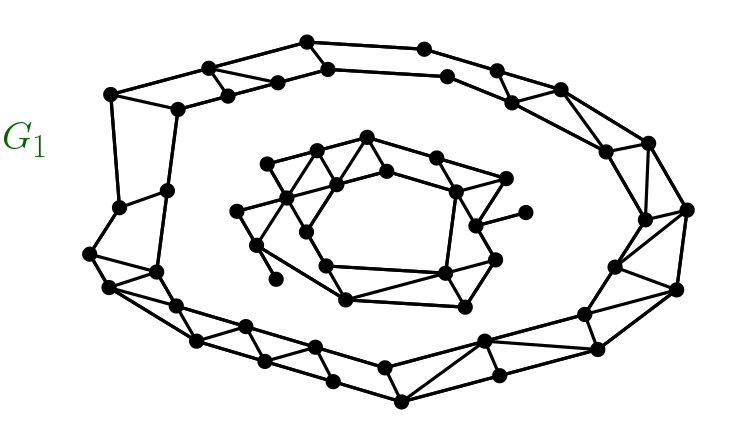
\includegraphics[height=4cm]{images/onion4.png}}
        \only<5>{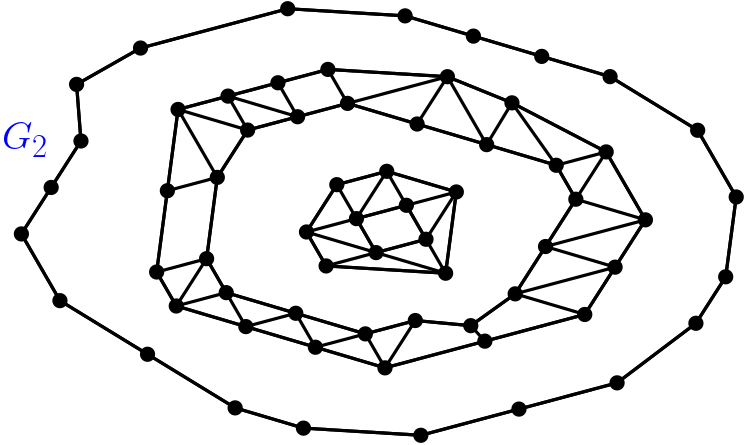
\includegraphics[height=4cm]{images/onion5.png}}
    \end{minipage}
\end{frame}

\begin{frame}{Solucionando $G_i$}
    \centering\Large
    Usamos o Lema 1 em cada componente.
\end{frame}

\begin{frame}{Solução Ótima para $G_i$}
    \centering\Large
    Para cada $i$, geramos uma solução ótima $X_i$ de $G_i$.
    \bigbreak
    O tempo total gasto é $2^{O(k)} \cdot n$.
\end{frame}

\begin{frame}{Solucionando $G$}
    \centering\Large
    Basta retornar o $X_\alpha$ de maior cardinalidade!
\end{frame}

\begin{frame}{Corretude}
    \pause
    \setbeamercovered{transparent} % fade-in/fade-out lists
    \begin{proof}
        \begin{enumerate}
            \setlength\itemsep{1em}
            \item<2,8> Seja $O \subseteq V$ uma solução ótima;
            \item<3,8> Suponha que $|O| \ge k$;
            \item<4,8> $S_0, \dots, S_{\ell-1}$ particionam $V$;
            \item<5,8> Algum $i$ satisfaz $|O \cap V(G_i)| \ge k$;
            \item<6,8> $O \setminus S_i$ é independente em $G_i$;
            \item<7,8> Então $|X_\alpha| \ge |O \setminus S_i| = |O \cap V(G_i)| \ge k$.
        \end{enumerate}
        \alt<8>{\qedhere}{\phantom\qedhere}
    \end{proof}
\end{frame}


\section{Conclusão}
\begin{frame}{Outros Resultados}
    \begin{thm}[\cite{Cygan15}]
        Existem algoritmos FPT (parametrização natural) para os seguintes problemas em grafos planares:

        \begin{enumerate}[]
            \item Isomorfismo de Subgrafos;
            \item Bisseção Mínima.
        \end{enumerate}
    \end{thm}
\end{frame}

\begin{frame}{Resultado Geral}
    A única propriedade dos grafos planares que utilizamos é serem fechados por menores e terem \textbf{\emph{largura arbórea local}} limitada.
    \pause \bigbreak
    Uma classe de grafos $\mathcal{G}$ tem \textbf{\emph{largura arbórea local}} limitada se, para todo $G \in \mathcal{G}$ e $v \in V(G)$, vale $tw(G_v^r) \le f(r)$, onde $G_v^r$ é o subgrafo induzido pelos vértices a distância até $r$ de $v$.
\end{frame}

\begin{frame}{Limitações}
    \centering
    A técnica de \emph{Shifting}/Baker é eficaz para problemas ``locais''~\dots
    \bigbreak\pause
    \dots~mas falha em casos como TSP ou Árvore de Steiner.
\end{frame}

\begin{frame}{Generalização}
    \centering\large
    \textbf{\emph{Decomposição por contração}} em grafos livres de $H$:
    \pause
    \bigbreak
    \begin{thm}[\cite{Dem11}]
        Para todo grafo fixo $H$, existe uma constante $c_H$ tal que, \pause
        para todo inteiro $k \geq 1$, qualquer grafo livre de $H$-menores pode ter suas arestas particionadas em $k + 1$ classes de cor, \pause
        de modo que a contração de qualquer uma dessas classes resulta em um grafo com largura arbórea no máximo $c_H \cdot k$.
        \pause
        \bigbreak
        Além disso, tal partição pode ser encontrada em tempo polinomial.
    \end{thm}
\end{frame}

\begin{frame}
    \textbf{Exercício.} Apresente, usando a técnica de \emph{shifting}, um algoritmo FPT para o problema do Empacotamento Máximo de Triângulos (vértices disjuntos) em grafos planares.
    \pause

    \vfill
    \centering
    \LARGE{\centerline{Obrigado a todos pela atenção...}}
    \Huge{\centerline{Alguma Dúvida?}}
\end{frame}

%-----------------------[ Bibliography ]---------------------------------------%

\appendix

\beamerdefaultoverlayspecification{}
\setbeamertemplate{bibliography item}[text]
\begin{frame}
  \frametitle{Bibliografia}
  {
    \tiny
    \bibliographystyle{alpha}
    \bibliography{bibliography}
  }
\end{frame}

%-----------------------[ Backup ]---------------------------------------------%


\end{document}
